\documentclass[11pt]{report}
\usepackage[margin=1.3in]{geometry}
\usepackage[utf8]{inputenc}
\usepackage[italian]{babel}
\usepackage{amsmath}
\usepackage{afterpage}
\usepackage{amssymb}
\usepackage{svg}
\usepackage{listings}
\usepackage{float}
\usepackage{graphicx,wrapfig,lipsum}
\usepackage[makeroom]{cancel}
\usepackage{blindtext}
\usepackage{multicol}
\usepackage{hyperref}
\usepackage{pdfpages}

\usepackage{framed} 

\setcounter{tocdepth}{3}
\setcounter{secnumdepth}{3}

\usepackage[
type={CC},
modifier={by-nc-sa},
version={4.0},
]{doclicense}

\begin{document}
	\title{\textbf{Appunti di  Crittografia A.A.2020-2021}\\(basato sulla dispensa di \href{https://github.com/drw0if/Appunti/tree/main/Crittografia}{Aleandro Prudenzano})}
	\author{Gabriele Frassi (\textbf{g.frassi2@studenti.unipi.it})}
	%\date{A.A. 2020-2021}
	\maketitle
	
	\noindent \emph{FORSE LO AVETE FATTO A MATEMATICA DISCRETA} (cit. Bernasconi)
	
	\doclicenseThis
		
	\thispagestyle{empty}
	\clearpage 
	
	\setcounter{page}{1}
	
	\tableofcontents
	
	\chapter{Alcuni dettagli sul corso}
\paragraph{Obiettivo del corso e argomenti}
\[\boxed{\text{L’obiettivo del corso è comprendere le nozioni moderne dei cifrari moderni.}}\]
\begin{itemize}
	\item Faremo ciò da un punto di vista algoritmico, affrontando prima i cifrari storici . Sono richieste nozioni di algoritmica, ma anche di complessità computazionale. 
	\item Vedremo che alla base di un qualunque meccanismo di cifratura serve una chiave, e per tale motivo entreremo nel concetto di casualità e di numeri casuali: la casualità è necessaria per avere buone chiavi.
	
	\item Vedremo cifrari perfetti, che ci proteggono in modo completo se usati in modo corretto (soluzione ideale, anche se con un costo molto elevato facendo riferimento alla generazione delle chiavi).
	
	\item Vedremo cifrari simmetrici, cifratura a chiave pubblica di prima generazione (RSA) e seconda generazione (crittografia su curve ellittiche).
	
	\item Affronteremo anche il protocollo di autenticazione e le firme digitali, soffermandoci brevemente sul protocollo SSL.
	
	\item Concluderemo con argomenti più avanzati:
	\begin{itemize}
		\item protocollo “Zero Knowledge”;
		\item	elementi su valute virtuali e blockchain;
		\item	elementi di crittografia quantistica (protocollo per lo scambio delle chiavi, basato sui principi della meccanica quantistica).
	\end{itemize}
	Le nozioni relative all’ultimo punto non hanno nulla a che vedere col computer quantistico.
\end{itemize}
\paragraph{Libro suggerito}
Per seguire il corso è suggerito il libro 
\[\boxed{\text{Bernasconi, Ferragina, Luccio, Elementi di crittografia, Pisa Università Press 2015}}\]
I diritti d’autore, molto bassi, sono devoluti all’associazione \textit{Medici senza frontiere}.

\part{Introduzione}
\chapter{Introduzione alla crittologia}
\section{Crittografia e crittoanalisi}
Il termine crittografia significa “scrittura nascosta”. Distinguiamo due tipologie di studi:
\begin{itemize}
	\item \textbf{Crittografia} (metodi di cifratura).\\
	Studio di tecniche matematiche per mascherare messaggi, rendendoli incomprensibili a chi non è il legittimo destinatario.
	\item \textbf{Crittoanalisi} (metodi di interpretazione).\\
	Studio di tecniche matematiche per svelare messaggi criptati (si forza, si cerca di recuperare informazioni nascoste quando non si è il legittimo proprietario).
\end{itemize}
\noindent L’unione dei due termini da origine a un termine poco utilizzato: \textbf{crittologia}, lo studio della comunicazione su canali non sicuri e relativi problemi. La concezione del termine crittografia non è stretta: con questo termine facciamo molto spesso riferimento anche a questioni di crittoanalisi. 

%La crittografia (scrittura nascosta) è lo studio \emph{delle tecniche matematiche per mascherare i messaggi} a differenza della \emph{crittoanalisi} che tenta di svelarli.
%Esiste un termine più generico che li comprende: \emph{crittologia}.
\section{Scenario tipico della crittografia}
Il tipico scenario in cui ci poniamo è quello in cui Alice e Bob vogliono comunicare un messaggio \emph{m} su un canale insicuro dove è possibile intercettare i messaggi. Decidono quindi di adottare un \textbf{metodo di cifratura} che trasforma m in \emph{c} (\emph{c} è detto \textbf{crittogramma}), che deve essere:
\begin{itemize}
    \item \textbf{incomprensibile} al crittoanalista (Eve - Eavesdropper d'ora in poi)
    \item \textbf{facilmente decifrabile} da Bob
\end{itemize}

\subsection{Funzione di cifratura (criptaggio)}
L'operazione con la quale si trasforma m in c è di fatto una funzione:
$$
    C: \text{msg} \longrightarrow \text{critto}
$$
La funzione è applicata da chi spedisce il messaggio. Si passa dallo spazio dei messaggi allo spazio dei crittogrammi: chiaramente a un messaggio deve essere associato uno e un solo crittogramma (ricordare la definizione di funzione matematica\footnote{Da Wikipedia. In matematica, una funzione è una relazione tra due insiemi, chiamati dominio e codominio della funzione, che associa a ogni elemento del dominio uno e un solo elemento del codominio.}).
\subsection{Funzione di decifratura (decifrazione)}
L'operazione inversa:
$$
    D: \text{critto} \longrightarrow \text{msg}
$$
La funzione è applicata da chi riceve il messaggio e vuole decifrarlo. Si passa dallo spazio dei crittogrammi allo spazio dei messaggi. 
\subsection{Schema di comunicazione}
$$
    \text{Alice}: m \xrightarrow{C} c \xrightarrow[\text{canale insicuro}]{c} c \xrightarrow{D} m : \text{Bob}
$$
Si noti che per funzionare \emph{C} e \emph{D} devono essere in tempo polinomiale mentre per il crittoanalista, noto \emph{c}, deve essere esponenziale il tempo utile per riottenere \emph{m}.
\paragraph{NB} \emph{C} e \emph{D} devono essere l'una l'inversa dell'altra:
$$
    D(c) = D(C(m)) = m
$$
quindi \emph{C} è iniettiva: m diversi vanno in c diversi (altrimenti il destinatario Bob non potrà determinare in modo univoco il messaggio a lui rivolto).

\section{Esempi antichi}
\paragraph{Erodoto in "Storie" (V secolo a.C.)} Si prende un servitore, si rasano i suoi capelli e si scrive il messaggio sulla sua testa, si aspetta che la ricrescita lo copra e poi si spedisce il servitore verso Bob che dovrà solamente rasarlo nuovamente.

\paragraph{Spartani (V secolo a.C.)} Gli spartani (V secolo a.C.) usavano lo scitale che è un'asta cilindrica costruita in due esemplari identici posseduti dai due corrispondenti. Su un pezzo di pelle viene scritto il messaggio dopo averlo avvolto attorno al cilindro seguendo le linee di esso. La fettuccia viene poi fatta indossare da un'uomo che la porta al ricevente.

\paragraph{Enea Tattico (Grecia, IV Secolo a.C.)} Enea tattico dedica un intero capitolo ai metodi militari usati per scambiarsi i messaggi:
\begin{itemize}
    \item inviare un libro con alcune lettere sottolineate a formare il messaggio in chiaro
    \item sostituire le vocali con altri simboli
\end{itemize}

\paragraph{Cifrario di Cesare} Il Cifrario di Cesare è il più antico cifrario di concezione moderna. \emph{c} è ottenuto da \emph{m} sostituendo ogni lettera con quella a 3 posizioni più avanti:
\begin{align*}
	A &\longrightarrow D \\
	B &\longrightarrow E \\
	C &\longrightarrow F \\
	D &\longrightarrow G\\
	.. &\longrightarrow ..
\end{align*}
Nella decifrazione faremo la stessa cosa al contrario. La segretezza in questo caso dipende dalla conoscenza del metodo: se il metodo viene scoperto allora non può essere più utilizzato!

\section{Livello di segretezza}
I metodi crittografici si classificano in:
\begin{itemize}
    \item \textbf{per uso ristretto} (usati in ambito diplomatico e/o militare\footnote{Si tenga conto che maggiore è il numero di persone coinvolte, maggiore è il rischio che il segreto venga rivelato da persone che ne sono a conoscenza. }): in cui la parte segreta del meccaniscmo è ampia (C e D sono tenute segrete)
    \item \textbf{per uso generale} (rivolto alla crittografia di massa): in cui la parte segreta è molto limitata (si restringe alla sola \emph{chiave}, nota solo ai due endpoint della comunicazione)
\end{itemize}
NB: per i cifrari di massa quindi le regole sono pubblcihe, solo le chiavi sono segrete. \textbf{Occorre sempre pensare che il nemico conosca il sistema}. 

\paragraph{Proporzione} Maggiore è la dimensione della parte segreta del cifrario minore deve essere il numero delle persone a conoscenza della parte segreta.

\subsection{Ridefinizione delle funzioni di criptaggio e decifrazione}
Ridefiniamo quindi:
\begin{align*}
	c = C(m, k) && m = D(c, k)
\end{align*}
con \emph{k} chiave segreta diversa per ogni coppia di utenti.
Se non si conosce \emph{k} la conoscenza dell'algoritmo non deve permettere l'estrazione di informazioni dal crittogramma. Se una chiave viene divulgata basta generarne un'altra lasciando inalterati \emph{C} e \emph{D}.
Ovviamente l'insieme delle chiavi deve esere così grande da non essere rompibile tramite brute-force e deve essere scelta in modo casuale.
\[\text{NB: brute-force $\equiv$ \emph{attacco esauriente}}\]
\paragraph{Esempio} Se $|key| = 10^{20}$ ed un calcolatore impiegasse $10^{-6}$ secondi per calcolare $D(c, k)$ e verificarne la significatività occorrerebbero comunque milioni di anni per provarle tutte.\\NB: solo la grandezza dello spazio delle chiavi non è un buon indice per l'affidabilità di un cifrario, potrebbe sempre essere rotto matematicamente (la segretezza non deve dipendere esclusivamente dalla cardinalità dello spazio).

\section{Crittoanalisi}
Il crittoanalista può assumere uno dei seguenti comportamenti.
\begin{itemize}
    \item Comportamento \emph{passivo}: si limita ad ascoltare il canale
    \item Comportamento \emph{attivo}:  disturba le comunicazioni o modifica il contenuto dei messaggi
\end{itemize}
Gli attacchi hanno lo scopo di forzare il sistema, raggiungendo l’informazione protetta da quel particolare sistema. L'attacco al sistema crittografico può avere due esiti:
\begin{itemize}
	\item \textbf{successo}, si scopre la funzione D, o si trova la chiave (e quindi possiamo decifrare qualunque crittogramma);
	\item \textbf{successo limitato}, si scoprono informazioni parziali, ma sufficienti per comprendere il contenuto del messaggio.
\end{itemize}
\subsection{Tipologie di attacchi}
Gli attacchi dipendono dalle informazioni in possesso del crittoanalista:
\begin{itemize}
    \item \textbf{\emph{cipher text attack}} (solo testo cifrato): si hanno una serie di crittogrammi:
    \[c_{1}, \dots , c_{r}\]
    \item \textbf{\emph{known plain-text attack}} (testo in chiaro noto): il crittoanalista ha a disposizione delle coppie
    $$(m_{1}, c_{1}), \dots , (m_{r}, c_{r})$$
    i messaggi non sono scelti dal crittoanalista
    \item \textbf{\emph{chosen plain-text attack}} (testo in chiaro scelto): ci si procura una serie di coppie
    $$(m_{1}, c_{1}), \dots , (m_{r}, c_{r})$$
    relative a messaggi in chiaro scelti dal crittoanalista
\end{itemize}

\subsection{Attacchi man-in-the-middle}
Il crittoanalista si installa sul canale ed interrompe le comunicazioni dirette tra i due, le sostituisce con messaggi propri e convince ogni utente che quei messaggi provengono legittimamente dall'altro.
\[\text{\underline{Il crittoanalista si finge Alice agli occhi di Bob e viceversa.}}\]

%\section{Cifrari perfetti e definizione di cifrario inattaccabile}
%Si conoscono alcuni \textbf{cifrari perfetti} ma richiedono operazioni estremamente complesse, e quindi sono utilizzati in condizioni estreme. La definizione di \textbf{cifrario inattaccabile} si deve a \emph{Claude Shannon} ('45 ma pubblicato nel '49 per segreto di stato imposto dai britannici)
%\[\text{\underline{Il messaggio in chiaro ed il crittogramma sono completamente scorrelati tra loro}}\]
%\section{\emph{one-time pad}}Un esempio di cifrario sicuro è il \emph{one-time pad} che richiede:
%\begin{itemize}
%    \item una chiave diversa per ogni messaggio
%    \item perfettamente casuale
%    \item lunga quanto il messaggio
%\end{itemize}
%Come vanno generate? Come vanno scambiate? Emergono problematiche su:
%\begin{itemize}
%	\item dimensione del messaggio e della chiave;
%	\item metodologie per far scambiare le chiavi tra i due endpoint.
%\end{itemize}
%\section{Cifrari dichiarati sicuri}I cifrari utilizzati oggigiorno non sono perfetti ma sono comunque \textbf{dichiarati sicuri} perché inviolati e per violarli è necessario risolvere problemi matematici estremamente difficili (abbiamo solo algoritmi esponenziali), quindi è richiesto tanto tempo o calcolatori molto grandi: nella pratica la risoluzione è impossibile.

%\paragraph{NB} Non sempre è noto se l'algoritmo esponenziale è l'unico metodo o ce ne sono altri ancora non scoperti.

%\section{\emph{Advanced Encryption Standard} (AES)}
%Uno dei cifrari di oggi è l'\emph{AES} (Advanced Encryption Standard): è lo standard per le comunicazioni non classificate, pubblicamente noto ed implementabile. Usa chiavi brevi a 128 o 256 bit. E' un cifrario simmetrico a blocchi, cioè si usa la stessa chiave sia per cifrare che per decifrare.

%\paragraph{Novità} La chiave non è scelta dai partecipanti ma dai dispositivi elettronici utilizzati. Ad ogni sessione viene utilizzata una nuova chiave (la chiave non deve durare a lungo). 

%\paragraph{Domanda} Come trasmettere la chiave in maniera sicura evitando intercettazioni?

%\section{Distribuzione delle chiavi su canali insicuri}
%Nel 1976 è stato proposto un protocollo di creazione e scambio di chiavi su un canale insicuro senza la necessità che le due parti debbano essersi scambiate altre informazioni. Questo algoritmo è detto \emph{protocollo Diffie-Hellman} ed è tuttora usato largamente.

%\paragraph{NB} Inventato da Merkle e poi da Diffie ed Hellman. Questi stessi hanno anche creato il concetto di crittografia a chiave pubblica senza tuttavia fornire un'implementazione.

%\section{Cifrari simmetrici ed asimmetrici}
%Nei cifrari simmetrici la chiave è unica e usata sia per criptare che per decriptare, ed è nota solo ai due partner che devono averla concordata su un canale sicuro. Nei cifrari asimmetrici, invece, si usa una coppia di chiavi:
%\begin{itemize}
%    \item \emph{$K_{pub}$}: è pubblica e nota a tutti (un po' come un lucchetto, tutti possono chiuderlo);
%    \item \emph{$K_{priv}$}: è privata e nota solo a chi riceve.
%\end{itemize}
%Bisogna quindi creare delle coppie di chiavi per ogni persona che vuole comunicare. Più precisamente:
%\begin{align*}c = C(m, K_{pub})&&m = D(c, K_{priv})\end{align*}
%I sistemi simmetrici si dicono anche a chiave privata, mentre quelli asimmetrici si dicono a chiave pubblica.
%Per usare un meccanismo come crittografia asimmetrica è necessario l'uso di funzioni \emph{one-way trapdoor} cioè passare da \emph{m} a \emph{c} è facile ma decifrare \emph{c} (senza conoscere la chiave) è difficile.

%\section{RSA (Rivest–Shamir–Adleman)}
%Nel 1977 Rivest-Shamir-Adleman inventano un sistema a chiave pubblica basato sulla difficoltà nel fattorizzare grandi numeri in fattori primi.
%Usando un sistema a chiave pubblica si ha una comunicazione molti a uno in quanto tutti hanno $K_{pub}$ e possono quindi cifrare i messaggi, ma solo il destinatario può leggerli conoscendo $K_{priv}$. Altri vantaggi sono:
%\begin{itemize}
%    \item tra n persone le chiavi sono $2n$, con un cifrario simmetrico invece sarebbero $\frac{n(n-1)}{2}$
%    \item non è necessario lo scambio segreto di chiavi
%\end{itemize}
%Tuttavia sono molto più lenti e le chiavi sono molto lunghe. Sono soggetti ad attacchi di tipo \emph{chosen plain-text attack}.

%\section{Cifrari ibridi}
%Si usa un cifrario a chiave segreta per la comunicazione di massa ma la chiave viene scambiata tramite cifrari asimmetrici. Si hanno quindi:
%\begin{itemize}
%    \item chiavi piccole
%    \item chiave simmetrica randomica impossibile da prevedere tramite attacco di tipo testo in chiaro scelto
%\end{itemize}

%\section{Applicazioni moderne}
%Attualmente i protocolli crittografici sono usati per:
%\begin{itemize}
%    \item \emph{identificazione dell'utente}: si accerta l'identità
%    \item \emph{autenticazione dell'utente}: si accerta che il messaggio venga dalla persona che dice di averlo mandato
%    \item \emph{firma digitale}: permette di evitare che un utente che ha inviato un messaggio neghi di averlo fatto e si dimostra l'identità del mittente agli occhi del ricevente
%\end{itemize}

%\section{Svolte future}
%\begin{itemize}
%    \item trasmissione protetta sulla rete (OpenSSL)
%    \item moneta elettronica (protocollo Bitcoin)
%    \item protocolli zero-knowledge
%    \item protocolli di cifratura quantistici
%\end{itemize}
	\chapter{Rimandi alla teoria dell'informazione}
\section{Rappresentazione matematica di oggetti}
Per parlare di Crittografia dobbiamo introdurre alcune nozioni matematiche relative alla rappresentazione di oggetti. Rappresentare matematicamente un oggetto significa attribuirgli un nome: dobbiamo fare ciò in modo rigoroso.
\paragraph{Alfabeto} Un \emph{alfabeto} è un insieme finito di caratteri detti simboli. 
\subsection{Rappresentazione degli oggetti con l'alfabeto} Un oggetto è rappresentato da una sequenza ordinata di caratteri dell'alfabeto. A oggetti diversi corrispondono sequenze diverse ed il numero di oggetti rappresentabili è infinito (fissata una lunghezza qualsiasi posso sempre creare sequenze più lunghe). 
Fissato un alfabeto $\Gamma$ tale che $|\Gamma| = s$ (dove $s$ è il numero di caratteri dell'alfabeto) e fissati \emph{N} oggetti da rappresentare otteniamo:
\begin{itemize}
	\item $d(s, N)$: è la lunghezza della sequenza più lungha di un oggetto dell'insieme
	\item $d_{min}(s, N)$: valore minimo di $d(s, N)$ tra tutte le rappresentazioni possibili
\end{itemize}
Un metodo di rappresentazione è tanto migliore tanto più $d(s, N)$ si avvicina a $d_{min}(s, N)$.

\subsubsection{Alfabeto unario}
Prendiamo un alfabeto con un solo simbolo ($s=1$): $\Gamma = \{0\}$
\paragraph{Variazione di N} L’unica possibilità che abbiamo per costruire sequenze diverse è alterare la lunghezza $N$, visto che le sequenze sono solo ripetizioni dell’unico carattere presente nell’alfabeto (0, 00, 000, …). 
\[\Longrightarrow d_{min}\left(1,N\right)=N\]
La rappresentazione non è comoda, ma soprattutto è poco efficiente.


\subsubsection{Alfabeto binario}
Passiamo a un alfabeto con due caratteri ($s = 2$). 
\[\Gamma = \{0, 1\}\]
$\forall k \geq 1$ (dove $k$ è la lunghezza della sequenza) si hanno $2^{k}$ sequenze, quindi il numero totale di sequenze lunghe da 1 a k è (data la lunghezza $k$ consideriamo anche le possibili sequenze realizzabili con un numero di caratteri minori a $k$):
$$
\sum^{k}_{i=0} 2^{i} = 2^{k+1} - 2
$$
Nel risultato finale si ha $-2$ invece di $-1$ visto che non si considera $i=0$. Per $N$ oggetti da rappresentare imponiamo che il numero di sequenze possibili sia minimo uguale ad $N$:
\begin{align*}
	2^{k+1}-2 &\geq N\\
	2^{k+1} &\geq N+2\\
	(k+1)\log(2) &\geq \log(N+2)\\
	(k+1) &\geq \frac{\log(N+2)}{\log(2)}\\
	k&\geq \log_2(N+2)-1
\end{align*}
troviamo il minimo applicando l'operatore \emph{ceil}
$$ k_{min}=d_{min}(2, N) = \lceil \log_{2}(N+2) - 1 \rceil $$
$$ \lceil \log_{2}N \rceil - 1 \leq d_{min}(2, N) \leq \lceil \log_{2}N \rceil $$

\paragraph{Esempio} Facciamo un esempio con $N=7$ (vogliamo sette sequenze di caratteri diverse), abbiamo 
$\left\lceil{\log}_2{7}\right\rceil=3$, dunque possiamo costruire N sequenze differenti tutte di lunghezza $\left\lceil{\log}_2{7}\right\rceil$
\[000,\ 001,\ 010,\ 011,\ 100,\ 101,\ 110\]La cosa è importante nelle applicazioni crittografiche: parole di pari lunghezza per evitare l’uso di separatori (cioè simboli che mi segnalano la fine di una parola e l’inizio della successiva).


\subsubsection{Alfabeto $s-$ario}
Abbiamo un alfabeto caratterizzato da $s$ caratteri. Possiamo costruire N sequenze differenti tutte di $ \lceil \log_{s}N \rceil $ caratteri.

\paragraph{Esempio}  Supponiamo di avere $\Gamma$ e di voler generare $1000$ sequenze:
\[\text{$\Gamma = \{0, \dots, 9 \}$ $\implies$ $\lceil \log_{10}1000\rceil = 3 $ cioè i numeri da 000 a 999}\]
Usare sequenze tutte della stessa lunghezza è vantaggioso perché posso concatenare più oggetti senza usare un separatore. Si dice \textbf{rappresentazione efficiente} una rappresentazione che usa un numero massimo di caratteri di ordine logaritmico nella cardinalità dell'insieme da rappresentare (N) quindi bisogna avere almeno 2 caratteri.

\subsection{Rappresentazione di interi}
La rappresentazione degli interi è una rappresentazione di tipo posizionale, dove il valore del numero dipende anche dalla posizione. Risulta efficiente  indipendentemente dalla base $s \geq 2$ scelta perché un intero $N$ costituito da $d$ cifre soddisfa la seguente condizione: \[\lceil \log_{2}N \rceil \leq d \leq \lceil \log_{2}N \rceil + 1\]
Abbiamo il concetto di \textbf{riduzione logaritmica} tra il valore di un numero N e la lunghezza della sua rappresentazione. Per avere complessità polinomiale il numero di istruzioni dell’algoritmo deve crescere come il logaritmo del valore (e non come il valore!!!).
\section{Differenza tra calcolabilità e complessità}
A questo punto possiamo distinguere la teoria della calcolabilità da quella della complessità:
\begin{itemize}
	\item \textbf{Teoria della calcolabilità}\\La teoria della calcolabilità studia gli algoritmi da un punto di vista di risoluzione algoritmica: quali problemi possono essere risolti algoritmicamente in un calcolatore (problemi decidibili) e quali no (problemi non decidibili).
	\item \textbf{Teoria della complessità}\\La teoria della complessità studia gli algoritmi (problemi decidibili) da un punto di vista dell’efficienza (problema efficiente, complessità polinomiale, o problema intrattabile, complessità esponenziale)
\end{itemize}

\section{Teoria della calcolabilità}
La calcolabilità si occupa della potenza e dei limiti dei sistemi di calcolo. La disciplina ha un secolo di vita, nasce quando i logici matematici iniziano ad esplorare i concetti di computazione, algoritmo e risoluzione algoritmica di problemi. 
\subsection{Problemi computazionali}
I problemi a cui siamo interessati sono problemi computazionali, che hanno una formulazione matematica precisa e una risoluzione algoritmica. Si distinguono in:
\begin{itemize}
	\item \textbf{problemi non decidibili}, non risolvibili algoritmicamente in un calcolatore (ne è stata dimostrata l’esistenza prima della nascita del calcolatore);
	\item \textbf{problemi decidibili}, che ammettono una soluzione algoritmica. Se consideriamo la complessità distinguiamo questi problemi in
	\begin{itemize}
		\item \textbf{problemi trattabili} (algoritmi di costo polinomiale, esistono algoritmi di complessità polinomiale che ne permettono la risoluzione),
		\item \textbf{problemi intrattabili} (algoritmi di costo esponenziale, non solo non esistono algoritmi di complessità polinomiale, ma si è anche dimostrata l'esistenza di un limite inferiore),
		\item \textbf{problemi aventi stato computazionale non noto} (non esistono algoritmi di complessità polinomiale, ma non si è dimostrata l'esistenza di un limite inferiore - dunque potrebbero essere scoperti in futuro algoritmi aventi minore complessità).
	\end{itemize}
\end{itemize}


%\subsection{Insieme dei problemi trattabili}
%Tra i problemi decidibili abbiamo i problemi trattabili, ossia problemi risolvibili con algoritmi di complessità polinomiale:
%\begin{itemize}
%	\item	ricerca di chiavi in array, liste, alberi (algoritmo di ricerca lineare, ma anche algoritmo di ricerca binaria – più efficiente);
%	\item	problemi sui grafi, si pensi ad esempio alla ricerca di un ciclo Euleriano.
%\end{itemize}
%Per quanto riguarda i problemi non risolvibili con complessità polinomiale (sempre tra i problemi decidibili) si distinguono le due classi successive.

%\subsection{Insieme dei problemi intrattabili}
%I problemi intrattabili richiedono obbligatoriamente algoritmi di complessità esponenziale: presentano un limite inferiore (ripensare a quanto visto ad algoritmi), dunque non è possibile individuare algoritmi con complessità inferiore. Gli esempi classici sono:
%\begin{itemize}
%	\item generazione delle sequenze binarie e delle permutazioni (il numero di sequenze è esponenziale in numero, non posso impiegare un tempo minore);
%	\item torre di Hanoi (spostamento dei dischi dal primo al terzo piolo tenendo conto di alcune regole).
%\end{itemize}

%\subsection{Insieme dei problemi aventi stato computazionale non noto}
%Ci sono problemi il cui stato computazionale non è noto, per esempio la ricerca del cammino hamiltoniano. Sappiamo risolvere questi problemi (sono problemi decisionali) con algoritmi di complessità esponenziale, ma contrariamente a prima non abbiamo un limite inferiore: nessuno ha dimostrato in modo rigoroso che non esistono problemi di complessità inferiore. 


\subsection{Esistenza di problemi non decidibili}
Vogliamo dimostrare l'esistenza di problemi non decidibili.
\subsubsection{Definizione: insiemi con stessa cardinalità}
Due insiemi $A$ e $B$ hanno la stessa cardinalità 
\[|A|=|B|\]
\emph{se e solo se} si può stabilire una corrispondenza biunivoca tra i loro elementi (una mappa)\footnote{Rinfreschiamoci la memoria sulla biunivocità grazie a Wikipedia: in matematica una corrispondenza biunivoca tra due insiemi X e Y è una relazione binaria tra X e Y, tale che ad ogni elemento di X corrisponda uno ed un solo elemento di Y, e viceversa ad ogni elemento di Y corrisponda uno ed un solo elemento di X. In particolare, la corrispondenza biunivoca è una relazione di equivalenza.}.
\subsubsection{Definizione: insieme numerabile} Un insieme è \emph{numerabile} (ha una infinità numerabile di elementi) \emph{se e solo se} i suoi elementi si possono mettere in corrispondenza biunivoca con i numeri naturali.
\begin{itemize}
	\item Un insieme numerabile può essere elencato: \[a_1, a_2, \dots, a_n, \dots\]
	\item Le stringhe di lunghezza finita di simboli di un alfabeto finito sono un insieme numerabile
	\begin{itemize}
		\item Il numero di queste stringhe è infinito, ma la cosa importante è che \textbf{ogni sequenza dell’elenco abbia una distanza finita dall’inizio} (cioè deve essere possibile raggiungere qualsiasi sequenza attraverso un numero finito di passi dalla prima sequenza).
		
		\item Usiamo l'\emph{ordinamento canonico}:
		\begin{itemize}
			\item si ordinano le sequenze per lunghezza crescente
			\item le sequenze di pari lunghezza si ordinano alfabeticamente (supponendo di avere creato una regola di ordine tra i caratteri)
		\end{itemize}
		
		Quindi una sequenza $s$ arbitraria si troverà tra quelle $|s|$, posizione alfabetica tra queste.
		
		\item \textbf{Esempio}.
		\begin{align*}
			&\Gamma=\{a,b,c,\dots,z\}\\
			&a,b,c,\dots,z\\
			&aa,ab,\dots,az,ba,\dots,bz,\dots,za,\dots,zz\\
			&aaa,aab,\dots,baa,\dots,zaa,\dots,zzz\\
			&aaaa,\dots
		\end{align*}		
		Seguendo questo metodo ogni sequenza corrisponde ad un numero $\in \mathbb{N}$ ed ogni naturale ha una sequenza associata.
		\item \textbf{Attenzione}. Questo si può fare perché abbiamo preso sequenze di lunghezza finita, per sequenze di lunghezza infinita non esiste una enumerazione.
	\end{itemize} 
	\item \textbf{Esempi di insiemi non numerabili}.
	\begin{itemize}
		\item $\mathbb{R}$ e sottoinsiemi (per esempio $\mathbb{R}$ ristretto a $(0, 1)$ o $[0, 1]$)
		\item \underline{\textbf{insieme delle funzioni in una o più variabili}}
	\end{itemize}
\end{itemize}



\subsubsection{Dimostrazione} Dimostriamo per quanto riguarda l'ultimo insieme citato tra i non numerabili. 
\begin{itemize}
	\item Un problema computazionale può essere visto come una funzione matematica che associa ad ogni insieme di dati su $k$ numeri interi il risultato su $j$ numeri interi:
	$$ f :  \mathbb{N}^{k} \longrightarrow \mathbb{N}^{j} $$
	Se siamo in grado di dimostrare che questo insieme di funzioni non è numerabile allora possiamo dire la stessa per l’insieme di problemi computazionali.
	\item Per semplificarci la vita dimostriamo la cosa su un sottoinsieme
	\[F = \{f | f: \mathbb{N} \longrightarrow \{0, 1\}\}\]
	Ogni $f \in F$ può essere rappresentata da una sequenza infinita:
	\begin{table}[!h]
		\centering
		\begin{tabular}{c|c|c|c|c|c|c|c}
			$x$ & 0 & 1 & 2 & 3 & \_ & n & \_  \\
			\hline
			$f(x)$ & 0 & 1 & 0 & 1 & \_ & 0 & \_
		\end{tabular}
	\end{table}
	
	oppure da una regola finita di costruzione:
	
	\[f(x) =
	\begin{cases}
		$0 \text{se x è pari}$ \\
		$1 \text{se x è dispari}$
	\end{cases}\]
	\item Supponiamo per assurdo che $F$ sia numerabile, quindi è possibile trovare una enumerazione per $f \in F$: questo significa poter associare un numero progressivo nella numerazione e costruire una tabella avente un numero infinito di righe (possibili funzioni) e colonne (possibili valori in ingresso).
	\begin{table}[!h]
		\centering
		\begin{tabular}{c|c c c c}
			$x$ & 0 & 1 & 2 & \_  \\
			\hline
			$f_0(x)$ & 1 & 0 & 1 & \_ \\ 
			$f_1(x)$ & 0 & 0 & 1 & \_ \\ 
			$f_2(x)$ & 1 & 1 & 0 & \_ \\ 
		\end{tabular}
	\end{table}
	\item Per dimostrare la non numerabilità dell'insieme mi basta individuare una sola funzione non numerabile. Consideriamo dunque la seguente funzione:
	
	\[g(x) = 
	\begin{cases}
		$0 \text{ se }$ f_x(x) = 1 \\
		$1 \text{ se }$ f_x(x) = 0 \\
	\end{cases}\]
	$g \in F$ perché è una funzione dai naturali a \{0, 1\} ma non può corrispondere a nessuna delle funzioni nella tabella precedente:
	\begin{itemize}
		\item non può essere $f_0$ in quanto differisce in $x = 0$
		\item non può essere $f_1$ in quanto differisce in $x = 1$
		\item e così via $\forall n$
	\end{itemize}
	\item Diciamo la cosa in modo più formale:
	\begin{itemize}
		\item Supponiamo per assurdo che esista un valore $i$ tale che $f_i \equiv g$.
		\item Possiamo dire che $f_i\equiv g$, tuttavia per definizione
		\[g(j)=\begin{cases}0&f_j(j)=1\\1&f_j(j)=0\end{cases}\]
		Quanto scritto consiste di fatto nella funzione di complementazione, quindi per forza ho $g\left(j\right)\neq f_j\left(j\right)$. Noi abbiamo considerato la diagonale, ma nulla ci vieta di considerare linee arbitrarie che attraversano la tabella toccando tutte le righe e tutte le colonne esattamente una volta.
		\item Per qualunque numerazione scelta esiste sempre almeno una funzione esclusa, dunque ${F}$ non è numerabile.
		\item Se $F$ è un insieme non numerabile allora tutti gli insiemi che lo contengono non sono numerabili:
		\begin{itemize}
			\item $f:\mathbb{N} \to \mathbb{N}$
			\item $f:\mathbb{N} \to \mathbb{R}$
			\item $f:\mathbb{R} \to \mathbb{R}$
			\item $f:\mathbb{N}^k\to \mathbb{N}^j$ (insieme delle funzioni in una o più variabili)
		\end{itemize}
		\textbf{L'insieme dei problemi computazionali non è numerabile}!
	\end{itemize}
\end{itemize}

\subsubsection{Conclusioni: il problema della rappresentazione}
L'informatica rappresenta tutte le sue entità in forma digitale come "sequenze finite di simboli di alfabeti finiti". Possiamo dire quindi che la conoscenza umana è numerabile. L'algoritmo è una sequenza finita di operazioni, completamente e univocamente determinate. La formulazione di un algoritmo dipende dal modello di calcolo utilizzato: se uso la macchina di Turing ho una codifica, se uso il C ne ho un'altra, ecc. Qualsiasi codifica si scelga gli algoritmi sono sempre descritti da una sequenza finita di caratteri di un alfabeto finito. 

\paragraph{In conclusione}
\begin{itemize}
	\item L'insieme degli algoritmi è infinito ma numerabile.
	\item \underline{I problemi computazionali sono infiniti ma non numerabili}.
\end{itemize}
Se l'insieme dei problemi computazionali non è numerabile allora non è possibile stabilire una corrispondenza biunivoca tra insieme dei problemi computazionali e quello degli algoritmi, ergo \textbf{esistono problemi computazionali non associati a un corrispondente algoritmo di calcolo} (ricordare quanto detto all'inizio su due insiemi che hanno la stessa cardinalità).

$\hfill\blacksquare$

\subsection{Problema dell'arresto (Halt problem) e sua indecidibilità}
Il problema dell’arresto è un problema indecidibile, individuato da Alan Turing nel 1930. 
\begin{itemize}
	\item Presi ad arbitrio un algoritmo A e i suoi dati di input d, dobbiamo decidere in tempo finito (volendo anche esponenziale, basta che sia finito) se la computazione di A su d termina (il programma termina la sua esecuzione) o non termina (va in loop, cioè continua a ripetere la stessa sequenza di istruzioni all’infinito ).
	\item In sostanza vogliamo individuare \textbf{un algoritmo che indaga sulle proprietà di un altro algoritmo}, cioè un algoritmo che ha come input un altro algoritmo. 
	\begin{itemize}
		\item Un algoritmo A, comunque formulato, può operare sulla rappresentazione di un altro algoritmo B. Poniamo quindi A(B).
		\item Possiamo fare anche A(A), per esempio se l’algoritmo A deve calcolare la lunghezza del file che rappresenta l’algoritmo.
	\end{itemize}
\end{itemize}
\paragraph{Dimostrazione di Turing sull'indecibilità del problema}
\begin{itemize} 
	\item Anche questa volta ragioniamo per assurdo: supponiamo che esista un algoritmo ARRESTO che prende A e d come input, e determina la risposta in tempo finito. In particolare
	\[\text{ARRESTO}(A,d)=\begin{cases}1&A(d)\text{ termina}\\0&A(d)\text{ non termina}\end{cases}\]
	Risulta scontato che l’algoritmo non deve consistere nell’eseguire il programma: questo perché se il problema non si arresta allora la funzione non può restituire 0 in tempo finito.
	\item Immaginiamo $D=A$, quindi $A(A)$ (algoritmo che ha come input se stesso). Possiamo dire
	\[\text{ARRESTO}\left(A,A\right)=1\Longrightarrow A\left(A\right)\mathrm{\ termina}\]
	fin qui nulla di strano.
	\item Se esiste l’algoritmo ARRESTO allora esiste il seguente algoritmo PARADOSSO:
	\begin{verbatim}
		PARADOSSO(A): while(ARRESTO(A,A)) { }
	\end{verbatim}
	la condizione nel while è true e non viene influenzata dal corpo (non cambia).
	\item L'algoritmo $\text{PARADOSSO}(A)$ non termina se l'algoritmo $A(A)$ termina, cioè se abbiamo $\text{ARRESTO}\left(A,A\right)=1$. Posso dire che $\text{PARADOSSO}(A)$ termina solo se $A(A)$ non termina.
	\[\text{PARADOSSO}\left(A\right)\mathrm{ termina}\Longleftrightarrow x=\text{ARRESTO}\left(A,A\right)=0\]
	\item Consideriamo $\text{PARADOSSO}(\text{PARADOSSO})$: osservo che termina solo se 
	\[\text{PARADOSSO}\left(\text{PARADOSSO}\right)\mathrm{termina}\Longleftrightarrow x=\text{ARRESTO}\left(\text{PARADOSSO},\ \text{PARADOSSO}\right)=0\]
	Ecco la contraddizione: stiamo dicendo che $\text{PARADOSSO}\left(\text{PARADOSSO}\right)$ termina solo se $\text{PARADOSSO}\left(\text{PARADOSSO}\right)$ non termina. La contraddizione può essere risolta solo affermando la non esistenza di PARADOSSO, dunque non può esistere nemmeno ARRESTO.
\end{itemize}
$\hfill\blacksquare$

\noindent Un algoritmo ARRESTO sarebbe uno strumento estremamente potente: permetterebbe, ad esempio, di dimostrare congetture ancora aperte sugli interi (esempio: la congettura di Goldbach\footnote{Da Wikipedia. In matematica, la congettura di Goldbach è uno dei più vecchi problemi irrisolti nella teoria dei numeri. Essa afferma che ogni numero pari maggiore di 2 può essere scritto come somma di due numeri primi (che possono essere anche uguali).}).


\subsection{Problema indecidibile: equivalenza tra programmi}
\[\boxed{\text{E' indecidibile stabilire l'equivalente tra due programmi (stesso input $\implies$ stesso output)}}\]
Turing afferma che non esistono algoritmi che decidono il comportamento di altri algoritmi esaminandoli dall’esterno, cioè senza passare dalla loro simulazione.

\subsection{Modelli di Calcolo e complessità (tesi di Churc-Turing)}
Poniamoci una domanda
\[\text{\underline{La decidibilità dipende dal modello di calcolo o è una caratteristica del problema?}}\]
La domanda può essere posta in altri modi:
\begin{itemize}
	\item i linguaggi di programmazione esistenti sono tutti equivalenti? 
	\item esistono linguaggi più potenti e/o più semplici di altri? 
	\item ci sono algoritmi descrivibili in un linguaggio, ma non in un altro? 
	\item è possibile che problemi attualmente irrisolvibili possano essere risolti in futuro con altri linguaggi o con altri calcolatori?
\end{itemize}
Non abbiamo un teorema che ci permetta di rispondere in modo univoco alle domande precedenti, ma abbiamo una tesi secondo cui il modello di calcolo non influisce sulla decidibilità (tesi di Churc-Turing): \textbf{tutti i ragionevoli modelli di calcolo risolvono esattamente la stessa classe di problemi}. 
\paragraph{Significato} Questo significa che i modelli di calcolo si equivalgono nella possibilità di risolvere problemi (anche se con diversa efficienza), quindi incrementi qualitativi alla struttura di una macchina (anche al computer quantistico ), o alle istruzioni di un linguaggio di programmazione, servono solo a:
\begin{itemize}
	\item abbassare il tempo di esecuzione;
	\item rendere più agevole la programmazione.
\end{itemize}

\subsection{Algoritmi polinomiali ed esponenziali a confronto}
Perché si pone questa demarcazione netta tra algoritmi di costi polinomiale e algoritmi di costo esponenziale? 
Supponiamo di avere un calcolatore $C_1$ e un calcolatore $C_2$, entrambi hanno a disposizione un tempo t e devono risolvere lo stesso problema (per cui abbiamo lo stesso algoritmo risolutivo). Vogliamo vedere come cambia la dimensione dei dati trattabili a parità di tempo, in macchine con capacità computazionali diverse. Quindi:
\begin{itemize}
	\item $n_1$ sono i dati trattabili nel tempo $t$ su $C_1$, $n_2$ sono i dati trattabili nel tempo $t$ su $C_2$
	\item Usare $C_2$ per un tempo $t$ equivale a usare $C_1$ per un tempo $k\ \cdot t$
\end{itemize}
\begin{center}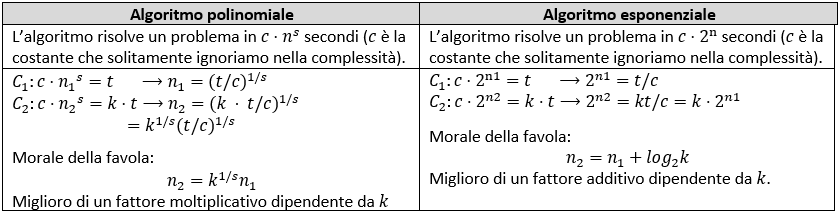
\includegraphics[scale=.9]{images/1.PNG}\end{center}
Si osserva che il miglioramento dell’algoritmo esponenziale è minore rispetto al miglioramento dell’algoritmo polinomiale. 
L’algoritmo efficiente è molto più importante della piattaforma hardware usata: 
\[\boxed{\text{Un algoritmo inefficiente lo è su qualunque piattaforma.}}\]

\section{Premessa alla teoria della complessità}
Per capire quanto è efficiente un algoritmo è necessario chiarire i parametri su cui valutare l'efficienza. Solitamente si prende a riferimento il tempo di esecuzione oppure l'occupazione di memoria. In entrambi i casi si descrive l'andamento attraverso una funzione matematica.
\begin{itemize}
	\item Successivamente dobbiamo determinare la variabile indipendente su cui si lavora: solitamente si prende il parametro $n$, che è la dimensione dell'ingresso (o dimensione dei dati). Il parametro indica la lunghezza della sequenza che specifica il valore dei dati per una particolare istanza del problema.
	\item Consideriamo la seguente funzione per la moltiplicazione
	\begin{verbatim}Molt(a,b)\end{verbatim}
	Supponiamo di avere i numeri $a=351, b=66$. Possiamo porre $n=5$ poichè le cifre tra i due numeri sono cinque. A questo punto sorge il problema che il numero di cifre dipende dalla base di rappresentazione adottata. Come risolviamo? Ripensiamo a quanto visto per la rappresentazione di oggetti attraverso sequenze finite costituite da caratteri di un alfabeto finito: per costruire $N$ sequenze differenti ho bisogno del seguente numero di caratteri
	\[\lceil \log_n N \rceil\]
	dove $n$ è il numero di caratteri dell'alfabeto. Il numero di caratteri dell'alfabeto è letteralmente la base (la base $n$ è costituita da $n$ cifre che vanno da $0$ ad $n-1$). Sappiamo che è possibile fare un cambio di base nel logaritmo con la seguente formula
	\[\log_c a = \frac{\log_b a}{\log_b c} \longrightarrow \left(\log_c a\right) \left(\log_b c\right) = \log_b a\]
	Questo significa che nel passaggio da una base a un'altra si va a moltiplicare per un fattore costante. Si consideri per esempio un intero: esso è rappresentato in base $10$ col seguente numero di cifre
	\[\lceil \log_{10}N \rceil\]
	Per passare dalla base $10$ alla base $2$ andrò a moltiplicare il numero di cifre per $\log_2 10$. Da questo deduciamo la necessità di ragionare per \textbf{ordini di grandezza}.
	\item L'ordine di grandezza è un insieme infinito che comprende tutte le funzioni che hanno un particolare comportamento rispetto a una funzione $g(n)$. Esse sono:
	\begin{itemize}
		\item $O(g(n))$, l'insieme di tutte le funzioni $f(n)$ per cui esistono due costanti positive $c,n_0$ tali che 
		$$f(n) \leq c g(n)$$
		questo $\forall n \geq n_0$. Al crescere di $n$ il comportamento della funzione $f(n)$ è limitato \textbf{\underline{superiormente}} dalla funzione $g(n)$
		\item $\Omega(g(n))$, l'insieme di tutte le funzioni $f(n)$ per cui esistono due costanti positive $c,n_0$ tali che 
		$$f(n) \geq c g(n)$$
		questo $\forall n \geq n_0$. Al crescere di $n$ il comportamento della funzione $f(n)$ è limitato \textbf{\underline{inferiormente}} dalla funzione $g(n)$
		\item $\Theta(n)$, l'insieme di tutte le funzioni $f(n)$ per cui esistono due costanti positive $c,n_0$ tali che
		$$c_1 g(n) \leq f(n) \leq c_2 g(n)$$
		questo $\forall n \geq n_0$. Al crescere di $n$ il comportamento della funzione $f(n)$ è limitato \textbf{\underline{superiormente}} e \textbf{\underline{inferiormente}} dalla funzione $g(n)$. Segue
		$$f(n)=\Theta(g(n)) \Longrightarrow f(n)=O(g(n)) \text{ e } f(n)=\Omega(g(n))$$
	\end{itemize}
\end{itemize}

\section{Teoria della complessità}
Possiamo immaginare un problema $\Pi$ come una funzione matematica $f: I \to S$, dove:
\begin{itemize}
	\item $I$: insieme delle \emph{istanze} di ingresso
	\item $S$: insieme delle \emph{soluzioni}
\end{itemize}
\subsection{Tipologie di problemi}
Alcune tipologie di problemi sono:
\begin{itemize}
	\item \textbf{Problemi decisionali}\\ Problemi dove l'insieme delle soluzioni è un insieme binario $S = \{0, 1\}$. 
	\begin{itemize}
		\item Un'istanza $x \in I$ è detta istanza positiva o accettabile se $\Pi(x) = 1$ 
		\item Un'istanza $x \in I$ è detta istanza negativa se: $\Pi(x) = 0$
		\item \textbf{Esempi}: numero primo, grafo connesso...
	\end{itemize}
	\item \textbf{Problemi di ricerca}\\Data un'istanza $x \in I$ vogliamo trovare una soluzione $s$ (trovare un cammino tra due vertici, ecc)
	\item \textbf{Problemi di ottimizzazione}\\Data un'istanza $x \in I$ si vuole trovare la migliore soluzione $s$ tra tutte quelle ammissibili (cammino minimo, ecc)
\end{itemize}
\subsection{Ruolo di problemi decisionali e di ottimizzazione nella teoria}
La teoria della complessità fa riferimento alla sola classe decisionale in quanto:
\begin{itemize}
	\item essendo $s = \{0, 1\}$ non ci si deve preoccupare del tempo per restituire la soluzione (influisce solo il tempo per il calcolo della soluzione);
	\item la difficoltà è già presente nella sua versione decisionale.
\end{itemize} 
Molti problemi di interesse pratico sono problemi di ottimizzazione. Possiamo esprimere i problemi di ottimizzazione in forma decisionale.
\paragraph{Esempio}
\begin{itemize}
	\item MAX-CLIQUE: trovare la clique più grande in un grafo G
	\item CLIQUE decisionale: esiste una clique in G di almeno k vertici? 	
\end{itemize}
CLIQUE decisionale non è più difficile di MAX-CLIQUE. Supponiamo di saper risolvere MAX-CLIQUE: se io so trovare la risposta allora automaticamente trovo risposta alla versione decisionale del problema.  Il problema di ottimizzazione è almeno tanto difficile quanto il corrispondente problema decisionale. Lo studio del problema decisionale permette di fornire un limite inferiore alla versione di ottimizzazione.

\subsection{Teoria della verifica}
\subsubsection{Concetto di \emph{certificato}}
In un problema decisionale siamo interessati a verificare se un'istanza del problema soddisfa una certa proprietà. In alcuni problemi è possibile fornire un certificato per ogni istanza accettabile, che ci convinca della sua accettabilità. Questo significa che non siamo tanto interessati alla soluzione nello specifico, ma a un qualcosa che attesti la sua esistenza.

\paragraph{Definizione} Si definisce il \textbf{certificato} come un attestato "breve" di esistenza di una soluzione con determinate proprietà (una descrizione succinta della soluzione), si definisce solo per le istanze accettabili (gli attestati di non esistenza non sono facili da costruire).

\subsubsection{Verifica in tempo polinomiale}
Nella teoria della verifica utilizziamo il costo della verifica di un certificato per una istanza positiva per caratterizzare la complessità del problema stesso. \paragraph{Definizione} Un problema $\Pi$ è \textbf{verificabile in tempo polinomiale} se
\begin{itemize}
	\item ogni istanza accettabile $x$ di $\Pi$ di lunghezza $n$ ammette un certificato $y$ di lunghezza polinomiale in $n$
	\item esiste un algoritmo di verifica polinomiale in $n$ ed applicabile ad ogni coppia \\$<x$, $y>$ che attesta se $x$ è accettabile.
\end{itemize}
\paragraph{Utilità della teoria della verifica ($\Pi \in NP$?)}  Quanto è effettivamente utile la teoria della verifica? Il dubbio può venire visto che il certificato è un qualcosa di molto vicino alla soluzione. La teoria della verifica ci aiuta a costruire una gerarchia di complessità dei problemi (cioè capire quanto un problema è facile o difficile), ma non aiuta nella risoluzione dei problemi stessi.
\begin{itemize}
	\item Chi ha una soluzione può verificare in tempo polinomiale se l’istanza è veramente accettabile (classe NP).
	\item Chi non ha una soluzione non ha il certificato e deve individuarlo. Lo faccio con metodo forza bruta: in tempo esponenziale considero tutti i casi possibili. 
\end{itemize}
Abbiamo introdotto la teoria della verifica per affrontare, poco più avanti, le classi NP ed NP-completo.

\subsection{Classi di complessità}
Dato $\Pi$ decisionale ed A algoritmo diciamo che A risolve $\Pi$ se, dato l'input $x$:
$$ A(x) = 1 \Longleftrightarrow \Pi(x) = 1 $$
Diciamo poi che A risolve $\Pi$ in tempo $t(n)$ ed in spazio $s(n)$ se il tempo di esecuzione e l'occupazione di memoria di A hanno andamento simile alle funzioni $t(n)$ e $s(n)$. Dato $f(n)$ diremo:
\begin{itemize}
	\item $\mathbf{Time(f(n))}$ \\
	Insieme dei problemi decisionali che possono essere risolti in tempo $O(f(n))$
	\item $\mathbf{Space(f(n))}$\\
	Insieme dei problemi decisionali che possono essere risolti in spazio $O(f(n))$
	\item \textbf{Classe P}.\\E' la classe di problemi che possono essere risolti in \textbf{\underline{AL PIU'}} tempo polinomiale nella dimensione dell'istanza di input.
	\begin{itemize}
		\item \textbf{Algoritmo polinomiale (tempo)}.
		Date due costanti $c,n_0>0$ tale che il numero di passi elementari è al più $n^c$ per ogni input di dimensione $n$ e per ogni $n>n_0$.
	\end{itemize}
	
	\item \textbf{Classe PSPACE}.\\
	Equivalente della classe P nello spazio. E' la classe di problemi che possono essere risolti in spazio polinomiale nella dimensione dell'istanza di input. 
	
	\item \textbf{Classe RP}.\\La classe di problemi \emph{Random-Polinomial} contiene tutti i problemi che ammettono un algoritmo di costo polinomiale randomizzato. Il test di primalità appartiene a questa classe.
	$$\boxed{P \subseteq RP \subseteq NP} $$
	
	\item \textbf{Classe EXP-TIME}\\
	La classe Exp(time) è la classe dei problemi risolvibili in  \textbf{\underline{AL PIU'}} tempo esponenziale nella dimensione $n$ dell'istanza di input.
	\[P\subseteq PSpace \subseteq Exp-Time\]
	
	NB: $P \subseteq PSpace$ perché un algoritmo polinomiale può accedere al più ad un numero polinomiale di locazioni di memoria (altrimenti dovrebbe essere esponenziale).
	
	NB: $PSpace \subseteq Exp-Time$ (abbiamo detto \textbf{\underline{AL PIU'}}, nota bene)
	
	Ad oggi non sappiamo se sono inclusioni proprie, l'unica separazione dimostrata è \[P \subset Exp-Time\] poiché abbiamo problemi risolti in $Exp$ e non in $P$ (ad esempio Hanoi)

	\item \textbf{Classe NP}\\
	NP è la classe dei problemi decisionali verificabili in tempo polinomiale.
	
	NB: NP sta per \emph{polinomiale su macchine non deterministiche}
	
	Abbiamo quindi che se si ha una soluzione essa è facile da verificare ma se non si ha una soluzione la si cerca in tempo esponenziale.
	
	NB: $P \subseteq NP$ certamente perché qualsiasi problema in P può essere risolto in tempo polinomiale. Non sappiamo però se $P \subset NP$ o $P = NP$. Per il momento la congettura pone $P \neq NP$
	\begin{center}
		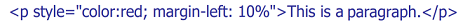
\includegraphics{images/2.PNG}
	\end{center}
	Si prenda ad esempio la SAT (lo vediamo nel dettaglio poco più avanti): è facile capire se dei valori soddisfano una formula logica, ma non è altrettanto facile individuare dei valori che soddisfano la formula logica stessa (forza brutta, analizzo tutte le possibili combinazioni).
	
	\item \textbf{Problemi NP-completi}\\
	I ricercatori, per cercare di rispondere al dilemma di P ed NP, hanno individuato all’interno della classe NP i problemi più difficili: la classe NP-completo.
	
	\underline{Questi problemi hanno una caratteristica comune}: se esistesse un algoritmo polinomiale per risolvere uno solo di questi problemi, allora tutti i problemi in NP potrebbero essere risolti in tempo polinomiale.
	
	La definizione è posta poco più avanti, a seguito della riduzione del concetto di \emph{riduzione polinomiale}.
\end{itemize}


\subsection{Riduzioni polinomiali}
Presi i problemi decisionali $\Pi_{1}$ e $\Pi_{2}$, con insiemi di input $I_{1}$ e $I_{2}$ (rispettivamente di $\Pi_{1}$ e di $\Pi_{2}$), diremo che il problema $\Pi_{1}$ si riduce in tempo polinomiale al problema $\Pi_{2}$ se esiste una funzione che mi trasforma una istanza del primo problema in una istanza del secondo problema $$f:I_{1} \to I_{2}$$
Essa è calcolabile in tempo polinomiale. Rappresentiamo la cosa con la seguente notazione:
$$ \Pi_{1} \leq_{p} \Pi_{2} $$
inoltre $$\boxed{x \text{ è accettabile per } \Pi_{1} \Longleftrightarrow f(x) \text{ è accettabile per } \Pi_{2}, \forall x \in \Pi}$$

\paragraph{Utilità} La riduzione polinomiale è utile perché supponendo di risolvere $\Pi_{2}$ in tempo polinomiale allora $\Pi_{1}$ viene tradotto in tempo polinomiale in $\Pi_{2}$ e quindi anche $\Pi_{1}$ è polinomiale:
$$ \Pi_{1} \leq_{p} \Pi_{2} \text{ e } \Pi_{2} \in P \Longrightarrow \Pi_{1} \in P $$
\subsection{Problema NP-arduo}
Un problema (non per forza decisionale) $\Pi$ si dice NP-arduo se ogni problema $\Pi' \in NP$ può essere risolto utilizzando $\Pi$ (riduco polinomialmente il problema $\Pi'$ al problema $\Pi$):
$$ \forall \Pi' \in \text{NP} \text{  } \Pi' \leq_{p} \Pi $$

\subsection{Problema NP-completo}
Un problema decisionale $\Pi$ si dice NP-Completo se
\begin{itemize}
	\item $\Pi \in \text{NP}$
	\item $\Pi$ è NP-arduo
\end{itemize} 
 Dimostriamo che se troviamo $\Pi$ NP-Completo, ma $\Pi \in P$ allora $\text{P}=\text{NP}$:
 \begin{itemize}
 	\item per ogni $\Pi' \in \text{NP}$ si ha $\Pi' \leq_p \Pi$, quindi trasformo $I_{\Pi'}$ in $I_{\Pi}$.
 	\item $I_{\Pi}$ è risolubile in tempo polinomiale, quindi qualunque $\Pi' \in \text{NP}$ è risolto in tempo polinomiale.
 \end{itemize}
$\hfill\blacksquare$

\subsection{Dimostrare che un problema è NP-arduo o NP-completo} Abbiamo visto che dimostrare $\Pi \in NP$ è semplice: basta esibire un certificato polinomiale (teoria della verifica). Non è semplice invece dimostrare che un problema è NP-arduo o NP-completo perché:
\begin{itemize}
	\item devo dimostrare che tutti i problemi NP si riducono a $\Pi$
	\item ma la prima definizione di NP-completo aggira il problema: il \emph{Teorema di Cook}
\end{itemize}

\subsection{Premessa al teorema di Cook: problema SAT}
Sia dato un insieme V di variabili logiche, definiamo:
\begin{itemize}
	\item \textbf{letterale}: una variabile o una sua negazione
	\item \textbf{clausola}: disgiunzione (OR) di letterali
	\item \textbf{espressione booleana in forma normale congiuntiva} (FNC): è una espressione logica formata da clausole unite da congiunzioni (AND di OR di variabili dirette o negate)
	
	Es: dati $ V = \{x, y, z, w\}$ una possibile FNC potrebbe essere: 
	$$(x \lor \bar{y} \lor z) \land (\bar{x} \lor w) \land y$$
	SAT si occupa di cercare dei valori di verità per rendere vera l'espressione. Nell'esempio la FNC è soddisfatta per 
	\begin{align*}
		x=1&&y=1&&z=0&&w=1
	\end{align*}
\end{itemize}
\paragraph{NB} Il problema c'è solo se l'espressione è FNC e passare ad un'altra forma richiede tempo esponenziale.

\paragraph{Risoluzione} Per risolvere iteriamo sulle $2^n$ possibili combinazioni e controlliamo la soddisfattibilità.
$$ \text{SAT} \in \text{Exp-Time}$$
quindi per risolvere questo ed altri problemi (clique, cammino hamiltoniano) è necessario iterare tra tutte le possibili combinazioni di ingresso? \emph{Non lo sappiamo}.

\subsection{Teorema di Cook}
Cook ha dimostrato che il problema SAT è NP-Completo. Dati un qualunque problema NP ed una qualunque istanza $x$ si può dimostrare che una espressione booleana in forma normale congiuntiva che descrive l'algoritmo del problema è sempre costruibile.

\paragraph{Conseguenza} \underline{Qualsiasi problema NP si riduce a SAT}. Per dimostrarle quindi che un problema è NP-completo ci basta prenderne uno che lo è e provare a ridurlo al problema in studio.

\paragraph{Esempio} Per dimostrare che clique è NP-completo cerchiamo un algoritmo polinomiale tale che:
$$ \text{SAT} \leq_{p} \text{CLIQUE} $$
se lo troviamo allora CLIQUE è NP-completo. SAT e CLIQUE sono NP equivalenti: \emph{tutti i problemi NP completi sono tra di loro NP equivalenti}.

\subsection{Classi co-P e co-NP}
C'è una profonda differenza tra certificare l'esistenza di una soluzione e certificarne la non esistenza. Dato un problema decisionale $\Pi$ possiamo definire un problema decisionale $co-\Pi$ che accetta tutte e solo le istanze rifiutate dal problema $\Pi$. 

\begin{itemize}
	\item \textbf{Insieme co-P}.\\
	Il problema co-$\Pi$ appartiene alla classe co-P. Si osservi che per ogni problema co-$\Pi$ appartenente alla classe co-P si ha co-$\Pi\in P$. Se il problema $\Pi$ è polinomiale allora anche il problema co-$\Pi$:\ risolvo il primo e complemento ottenendo il secondo (la cosa vale in entrambi i sensi). 
	
	\item \textbf{Insieme co-NP}.\\
	Come abbiamo l’insieme co-P per P abbiamo anche l’insieme co-NP per NP. Si osservi che per ogni problema decisionale co-$\Pi$ appartenente alla classe co-NP si ha co-$\Pi\in NP$. Contrariamente a prima si congettura che le due classi siano diverse (se ho il certificato di un problema non posso costruire direttamente il certificato del problema complementato): è solo una congettura, se questa fosse vera allora si potrebbe confermare che $P\ \neq NP$ (P è uguale al suo complementare, se dimostro che P è in realtà diverso si dimostra la disuguaglianza).
	\[\mathrm{P}\neq\text{co-}\mathrm{NP}\]
	Esempio: trovare ciclo hamiltoniano (NP) e trovare ciclo non-hamiltoniano (co-NP).
	
\end{itemize}
\begin{center}
	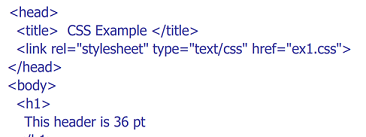
\includegraphics[scale=.8]{images/4.PNG}
\end{center}
\subsection{Recap sulla gerarchia delle classi}
\begin{center}
	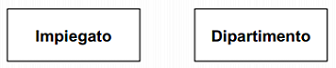
\includegraphics[scale=.8]{images/5.PNG}
\end{center}
\begin{itemize}
	\item La gerarchia si costruisce usando ciò che sappiamo con certezza (P contenuto in PSPACE) e le varie congetture.
	\item L’insieme più vasto è quello dei problemi decidibili.
	\item Abbiamo EXPTIME, all’interno del quale è presente PSPACE.
	\item All’interno di NP abbiamo P ed NP-completo. Un esempio di problema che non è P, ma neanche NP-completo, è la fattorizzazione (problema che ci interessa per la Crittografia). Questa cosa non è a caso: sulla macchina quantistica il problema è facilmente risolvibile.
\end{itemize}
Inoltre
\begin{itemize}
\item La classe P contiene problemi risolvibili in tempo polinomiale.
\item La classe NP contiene i problemi verificabili in tempo polinomiale (remember, verificare significa ottenere un certificato che attesta l'esistenza di una soluzione rispetto a una particolare istanza $I$)
\item I problemi NP-hard sono problemi a cui è possibile applicare il concetto di riduzione polinomiale: tutti i problemi appartenenti alla classe NP possono essere ridotti al problema NP-hard.
\item La classe NP-completo include tutti i problemi che appartengono ad NP e sono NP-hard. Se io risolvo uno di questi problemi risolvo tutti i problemi. Per verificare la possibilità di ridurre tutti i problemi di NP a un particolare problema uso il teorema di Cook, che afferma che qualsiasi problema NP si riduce a SAT: quindi se io posso ridurre SAT al problema in studio allora tutti i problemi NP possono essere ridotti al problema in studio.
\item Dato un problema posso definire il complementare, che accetta tutte le istanze rifiutate dal problema iniziale. Questo secondo problema appartiene alla classe co-P, ma anche a P. I problemi che appartengono ad NP appartengono anche a co-NP: si congettura che P $\neq$ co-NP (dato il certificato del problema iniziale non riesco a costruire automaticamente il certificato del problema complementato).
\end{itemize} 

	\part{Casualità e sequenze pseudocasuali}
\chapter{Casualità secondo Kolmogorov}
\section{Necessità di sequenze casuali}
Data una sequenza binaria vogliamo capire se questa è casuale oppure no. 
Ne abbiamo bisogno per vari motivi:
\begin{itemize}
	\item la generazione della chiave (deve essere imprevedibile);
	\item algoritmi randomizzati in Crittografia (algoritmi alimentati da sequenze casuali).
\end{itemize}

\section{Idea generale}
Poniamoci quindi un quesito: data una sequenza si vuole sapere se essa sia stata generata casualmente o meno. Consideriamo due sequenze binarie:
\begin{multicols}{2}
\begin{itemize}
    \item $h=111111111111\dots 1$
    \item $h'=101101101011\dots 0$
\end{itemize}
\end{multicols}
\noindent La prima sequenza può facilmente essere descritta come \emph{n volte 1}, mentre la seconda può essere descritta dettandola. La probabilità di generare ognuna le due sequenze è \[P(h)=P(h')=\left(\frac{1}{2}\right)^n=\frac{1}{2^n}\]
questo perchè la probabilità che esca $0$, ma anche $1$, in una cifra è $1/2$. Supponiamo di creare un algoritmo $A_h$ per generare la prima sequenza:
$$ A_h:\,<\text{scrivi $n$ volte $1$}> $$
L'unica cosa che varia è la lunghezza della sequenza $h$, quindi
\begin{align*}|h| = n && |A_h| = \log_2 |h|+c=\log_2n + c=O(\log n) \end{align*}
Lavoreremo con la seguente intuizione: \emph{una sequenza è casuale se non ammette un algoritmo di generazione la cui rappresentazione binaria sia più corta di h}. In parole povere: il modo più economico per definire una sequenza casuale è assegnare la sequenza stessa.

\section{Complessità in un sistema di calcolo}
I sistemi di calcolo (modello di calcolo astratto come una RAM, macchina di Turing, circuito di calcolo…, il luogo dove girano i nostri algoritmi) costituiscono un insieme infinito e numerabile: $S_1,S_2,\dots,S_i,\dots$. Dobbiamo scegliere un sistema di calcolo per mostrare che la casualità è indipendente. Scegliamo $S_i$ e supponiamo di avere un programma $p$ che genera una sequenza $h$ nel sistema di calcolo scelto. 
\subsection{Complessità di Kolmogorov} 
Definiamo la complessità di Kolmogorov di $h$ nel sistema $S_i$ come: 
$$
    K_{S_i}(h) = \min\{ |p| : S_i(p) = h \}
$$
cioè la lunghezza minima di un programma $p$ che nel sistema di calcolo $i-$esimo genera la sequenza $h$. \paragraph{Sequenza irregolare} Se la sequenza è irregolare il programma dovrà contenerla per intero, quindi anche il programma più piccolo che la genera sarà più lungo di $h$:
$$
    K_{S_i}(h) = |h| + c_i
$$
dove $c_i$ è la parte di programma che trasferisce in output la sequenza (dipende dal sistema di calcolo $i-$esimo scelto).

\subsection{Sistema di calcolo universale}
Per svincolarci dal sistema di calcolo consideriamo un sistema di calcolo universale $S_u$ che è in grado di simulare tutti i sistemi di calcolo esistenti:
$$
    S_i(p) = h \iff S_u(<i, p>) = S_i(p) = h
$$
Si ha quindi $q=<i,p>$, programma che genera la sequenza $h$ nel sistema universale $S_u$. Esso è lungo:
$$
    |q| = |i| + |p| = \lceil\log_2i\rceil + |p|
$$ 
Il primo termine dipende dall'indice del sistema e non dalla sequenza $h$ (è palesemente una costante, adottato un sistema $i$). E' logico derivare:
$$
    \forall h, \forall i : K_{S_u}(h) \leq K_{S_i}(h) + c_i
$$ 
dove $c_i$ dipende dal sistema di riferimento. La complessità del sistema universale per generare una sequenza $h$ è minore o uguale rispetto alla somma tra una costante e la {complessità del sistema $i-$esimo} per generare la solita sequenza.
\begin{itemize}
    \item L'uguaglianza si ha per quelle sequenze $h$ generate per simulazione di $S_i$, nel caso in cui non esistano algoritmi più brevi per $S_u$
    \item Il minore vale per le sequenze generabili con un programma più corto (per esempio simulando un altro sistema di calcolo $j \neq i$).
\end{itemize}
Dimentichiamoci per un attimo della costante: possiamo vedere che la complessità di Kolmogorov di una sequenza in un qualunque sistema di calcolo non potrà mai essere minore della complessità nel sistema di calcolo universale.
\[K_{S_i}(h) \geq K_{S_u}(h)\] Otteniamo un limite inferiore.

\paragraph{Quindi} Definiamo la complessità di Kolmogorov di una sequenza $h$ è quella nel suo sistema universale:
$$
    K(h) = K_{S_u}(h)
$$
Eliminiamo il pedice: non facciamo riferimento a un particolare sistema di calcolo.

\section{Definizione di casualità secondo Kolmogorov}
Una sequenza è casuale secondo Kolmogorov se:
$$
    K(h) \geq |h| - \lceil{\log_2|h|}\rceil
$$
Si conferma che la casualità è una proprietà della sequenza, indipendente dal sistema di calcolo adottato (e quindi dal modo in cui viene generata la sequenza).


\section{Esistenza di sequenze casuali di qualunque lunghezza}
Fissato la lunghezza $n$ abbiamo $S=2^n$ sequenze aventi tale lunghezza. Poniamo $T$ come numero di sequenze NON casuali di lunghezza $n$. Si vuole dimostrare che \[T < S\]cioè affermare che per ogni lunghezza $n$ esistono sequenze casuali.
\paragraph{Dimostrazione} Definiamo $N$ come numero di sequenze di lunghezza $ < n - \lceil \log_2n \rceil$ (sequenze che non rispettano la definizione di Kolmogorov), sono esattamente: \[N=\sum_{i = 1}^{n - \lceil \log_2n \rceil} 2^i = 2^{n - \lceil \log_2n \rceil} - 1\]
Tra queste N sequenze ci sono necessariamente anche le sequenze che descrivono i programmi $p$ per generare tutte le $T$ sequenze non casuali, quindi necessariamente si ha $T \leq N$. Chiaramente abbiamo $N < S$ e quindi
$$
T \leq N < S \longrightarrow T < S
$$
\paragraph{Osservazione} Al crescere di $n$ le sequenze casuali sono molto maggiori delle sequenze non casuali:
$$
    \frac{T}{S} \leq \frac{N}{S} = \frac{2^{n - \lceil \log_2 n \rceil} -1}{2^n} = \frac{1}{2^{\lceil \log n \rceil}} - \frac{1}{2^n} < \frac{1}{2^{\lceil \log n \rceil}}
$$
calcolando il limite concludiamo:
$$
    \lim_{n \to \infty} \frac{T}{S} = 0 \implies T << S
$$
Non solo $T$ è minore di $S$, ma le sequenze casuali per Kolmogorov sono maggioritarie.

$\hfill\blacksquare$
\section{Verifica della casualità di Kolmogorov problema indecidibile}
Purtoppo verificare la casualità di Kolmogorov è un problema indecidibile.
\paragraph{Dimostrazione} Supponiamo per assurdo che esista un algoritmo:
$$
    \text{RANDOM}(h) = 
    \begin{cases}
        1 $ se $h$ è casuale $\\
        0 $ altrimenti $
    \end{cases}
$$
Costruiamo l'algoritmo PARADOSSO che non ha parametri di input ed enumera tutte le possibili sequenze binarie in ordine di lunghezza crescente.
\begin{verbatim}
PARADOSSO:
    for binary h <- 1 to inf do{
        if( |h| - ceil(log2(|h|)) > |p| && RANDOM(h) == 1  )
           return h
    }
\end{verbatim}
Usiamo dal for non appena individuiamo una sequenza casuale e di dimensione maggiore della lunghezza $|p|$ definita come
$$
    |p| = |\text{PARADOSSO}| + |\text{RANDOM}|
$$
Si noti che $|p|$ è costante in quanto $n$ viene preso come parametro e non è presente all'interno del programma. Dato che \textbf{\underline{esistono sequenze casuali di qualunque lunghezza}} questo programma si fermerà sicuramente, fornendoci la prima sequenza casuale che soddisfa il vincolo di dimensione.  Attenzione all'assurdo:
\begin{itemize}
	\item si richiede che il programma sia di lunghezza breve e generi $h$;
	\item si richiede che la sequenza $h$ sia casuale.
\end{itemize}
\textbf{Con un programma di lunghezza breve non è possibile avere una sequenza $h$ casuale secondo Kolmogorov}. Ne segue quindi che $RANDOM$ non può esistere!
$\hfill\blacksquare$

	\chapter{Generatori pseudocasuali}
Abbiamo visto che esistono sequenze casuali per qualunque lunghezza arbitraria (secondo la definizione di Kolmogorov), ma che la verifica della casualità è un problema indecidibile. Oggi introduciamo \textbf{sequenze pseudocasuali}, facendo esempi pratici.
\section{Sorgente binaria casuale}
Una sorgente binaria casuale genera una sequenza di bit con le seguenti caratteristiche:
\begin{itemize}
	\item \textbf{Pari probabilità}.
	
	
	\[P(0)=P(1)=\frac{1}{2}\]
	vedremo che questa proprietà non è così vitale, possiamo indebolirla ponendo $P(0)>0, P(1)>0$ e immutabili durante il processo di generazione.
	\item \textbf{Generazione di un bit indipendente}.
	
	
	La generazione di un bit è indipendente dalla generazione degli altri. 
	Non posso prevedere il valore di un bit a partire da quelli già generati.
\end{itemize}
Prendiamo un caso dove $P(0)\ >\ P(1)$. Chiaramente la sequenza conterrà più 0 che 1. Supponiamo di avere la seguente sequenza
$$ 00|11|00|11|10|00|01|01|00 $$
Possiamo bilanciare la sequenza prendendo i bit a coppie. Elimino le sottosequenze uguali ed associo ad ogni coppia un valore 0 o 1:
\begin{align*}
01 \implies 0 && 10 \implies 1
\end{align*}
Otteniamo:
$$ 100 $$
Questa sequenza ottenuta sarà la nostra sequenza casuale.

\paragraph{Esistono vere sorgenti casuali?} Non è possibile garantire la perfetta casualità di una sorgente, e soprattutto l’indipendenza (generazione di bit indipendente da quella delle altre): ogni esperimento modifica l’ambiente, e quindi può influenzare gli esperimenti successivi. Dobbiamo accettare dei compromessi.


\section{Valutazione statistica}
Come possiamo valutare se il nostro generatore è valido da un punto di vista statistico? Vogliamo valutare le sequenze prodotte da un generatore pseudocasuale, cioè valutare se una certa sequenza presenta le proprietà tipiche di una sequenza casuale.Per simulazioni e algoritmi randomizzati sono necessari i seguenti test: 
\begin{itemize}
	\item \textbf{Test di frequenza}
	
	Verifica che le cifre siano presenti con la stessa frequenza
	\item \textbf{Poker test}
	
	Verifica che le sotto sequenze di lunghezza fissa siano distribuite in modo equo.
	\item \textbf{Test di autocorrelazione}
	
	Verifica che non ci siano regolarità nella sequenza ottenuta.
	\item \textbf{Run test}
	
	Verifica che le sottosequenze massimali di elementi tutti ripetuti abbiamo una distribuzione esponenziale negativa, cioè all’aumentare della loro lunghezza la frequenza decresce.
\end{itemize}
Per le applicazioni crittografiche si richiede anche il \textbf{test di prossimo bit}: test molto severo che implica tutti gli altri (nel senso che se si supera questo test gli altri sono sicuramente superati). Dobbiamo verificare l’impossibilità di fare previsioni sui bit prima che questi vengano generati.

\paragraph{Cosa si intende con test di prossimo bit?} Deve essere impossibile fare previsioni con risorse di calcolo polinomiali.
Un generatore binario supera il test di prossimo bit se non esiste un algoritmo polinomiale in grado di prevedere l’i+1-esimo bit della sequenza a partire dalla conoscenza degli i bit precedentemente generati con probabilità maggiore di $\frac{1}{2}$.

\paragraph{Algoritmo crittograficamente sicuro} Si dice che un generatore è crittograficamente sicuro se supera il test di prossimo bit. Il generatore lineare non supera questo test.
\clearpage 

\section{Generazione di sequenze brevi}
Vediamo alcune tecniche di generazione di sequenze brevi:
\begin{itemize}
    \item Fenomeni casuali presenti in natura (sorgenti di casualità tipo rumore del microfono)
    \item Processi software (come ad esempio la posizione della testina dell'hard disk o l'orologio del computer)
    \item Generazione mediante algoritmi matematici. Questo ultimo tipo costituisce i \textbf{generatori di numeri pseudo-casuali}. Non sono ovviamente sequenze casuali secondo Kolmogorov in quanto prodotte da un programma breve
\end{itemize}
Ci interessano questi ultimi generatori.
\subsection{Generatore di numeri pseudo-casuali}
\paragraph{Perchè pseudo?} Tipicamente questi algoritmi sono brevi e deterministici, quindi le sequenze ottenute non sono per nulla casuali secondo la teoria di Kolmogorov.

\paragraph{Input} Si parte dal seed, che è un piccolo valore casuale che l’utente può generare ricorrendo a sorgenti casuali, oppure lanciando una moneta. La casualità del seme viene usata per ottenere una sequenza più lunga.
\paragraph{Output} Flusso di bit arbitrariamente lungo, periodico (sottosequenza periodo al suo interno, che si ripete). Maggiore è la lunghezza del periodo, migliore è il generatore.

\paragraph{Numero di sequenze generabili}
\begin{itemize}
	\item Sia $S$ il numero di bit del seme.
	\item Sia $n$ la lunghezza della sequenza ottenuta col generatore.
\end{itemize}
Tipicamente $n>>S$. Si capisce che ci sono dei limiti: se io uso sempre lo stesso seme ho un algoritmo deterministico, viene generata sempre la solita sequenza “casuale”.
Il numero di sequenze diverse ottenibili dal seme è $2^S$, ma il numero di sequenze possibili con n bit è $2^n, 2^n>>2^S$


\subsection{Esempio di generatore pseudo-casuale: generatore lineare}
L'algoritmo non è valido per applicazioni crittografiche: i primi quattro test vengono superati, mentre il test di prossimo bit no. Questo perchè esistono algoritmi che osservando alcuni valori riescono a risalire ai parametri del generatore in tempo polinomiale.

\paragraph{Definizione} Il generatore lineare è definito dalla seguente equazione. Si consideri la $i-$esima cifra:
$$ x_{i} = \left( a \cdot x_{i-1} + b \right) \text{ mod } m $$
$a,b,m$ sono interi positivi. Il seme è il valore iniziale $x_0$ (che supponiamo di aver estratto casualmente). 
\paragraph{Periodo e permutazione} Data l'operazione modulo vogliamo ottenere una permutazione degli elementi appartenenti a $\mathbb{Z}_m = \{0,1,\dots,m-1\}$: per fare ciò dobbiamo massimizzare il periodo, e massimizzare il periodo significa ottenere un periodo lungo $m$. Ci servono:
\begin{itemize}
    \item $b$ ed $m$ coprimi, $\text{MCD}(b, m) = 1$;
    \item $(a-1)$ deve essere divisibile per ogni fattore primo di $m$;
    \item $(a-1)$ deve essere un multiplo di 4 se $m$ lo è.
\end{itemize}

\paragraph{Esempio} Valori $a=7, b=7, m=9$, seme $x_{0}=3$
\begin{align*}
	x_i = (7x_{i-1} + 7) \text{ mod } 9 \\\implies 3, 1, 5, 6, 4, 8, ... , 3
\end{align*}

\subsection{Generatore polinomiale, generalizzazione del precedente}
Vediamo la versione generalizzata del generatore lineare, dove si pone un polinomio. Anch'essa supera i primi quattro test ma non quello del prossimo bit.  E' nella forma:
$$ x_{i} = \left( a_{1}x_{i-1}^{t} + a_{2}x_{i-1}^{t-1} + ... + a_{t}x_{i-1} + a_{t+1} \right) \text{ mod } n $$
Possiamo utilizzarlo come generatore di sequenze binarie, dividendo per $n$:
\[
    r=\frac{x_{i}}{n} \longrightarrow
    \begin{cases}
        \text{Se la prima cifra decimale di $r$ è pari} \implies 0 \\
        \text{Se la prima cifra decimale di $r$ è dispari} \implies 1
    \end{cases}
\]

\subsection{Generatori crittograficamente sicuri con funzioni one-way}
Una funzione \emph{one-way} è una funzione facile da calcolare (tempo polinomiale) ma difficile da invertire (tempo esponenziale):
$$ x \xrightarrow{f(x)} y \text{ : tempo polinomiale} $$
$$ y \xrightarrow{f^{-1}(y)} x \text{ : tempo esponenziale} $$
Data una funzione $f$ one-way e dato un seme $x_{0}$ calcolo una sequenza:
\begin{center}
    \begin{tabular}{c | c c c c c}
        $S$: & $x$ & $f(x)$ & $f(x_{1}) = f(f(x))$ & ... & $f^{(n)}(x) = f(x_{n-1})$ \\
         & $x_{0}$ & $x_{1}$ & $x_{2}$ & & $x_{n}$ \\
    \end{tabular}
\end{center}
si prende il seme e si itera la funzione \textit{one-way} un numero arbitrario di volte. Il fatto è che ogni elemento della sequenza S si può calcolare polinomialmente dal precedente, ma non dai valori successivi (perché appunto la funzione è one-way). 
\paragraph{Problema} Se conosco x la sequenza è prevedibile! Risolviamo \emph{restituendo la sequenza al contrario}! Dato $x_{i+1}$ non possiamo calcolare facilmente $x_{i}$ ma solo $x_{i+2}$. Bisognerebbe passare per una funzione esponenziale ad ogni passo.

\subsection{Generatori binari crittograficamente sicuri}
Come faccio a trasformare un generatore crittograficamente sicuro definito sugli interi in un generatore crittograficamente sicuro che produce una sequenza binaria? Tipicamente le funzioni one-way non sono funzioni 0 e 1, quello che si fa è estrarre la complessità computazionale della funzione one-way sintetizzandola in un unico bit. Usiamo i cosiddetti \textit{predicati hard-core} delle funzioni one-way. 
\paragraph{Cosa intendiamo con predicato in generale?} \emph{Il predicato è una funzione che restituisce un valore vero o falso}
\paragraph{Definizione di predicato \emph{hard-core}} $b(x)$ si dice predicato hard-core di una funzione one-way se:
\begin{itemize}
    \item $b(x)$ è facile da calcolare conoscendo $x$
    \item $b(x)$ è difficile da prevedere conoscendo solo $f(x)$
\end{itemize}
\paragraph{Esempio} Consideriamo la funzione \emph{one-way}
$$ x \xrightarrow{} f(x) = x^2 \text{ mod } n \text{ (n non primo)} $$
Consideriamo il seguente predicato \emph{hard-core}
$$ b(x) = \text{"x è dispari"} $$
Se prendiamo i valori $n = 77, x = 10$ diventa facile calcolare 
$$f(x) = 10^{2} \text{ mod } 77 = 23$$
il contrario (conosciamo solo $f(x)$) prevede una enumerazione di tutti i valori da 0 a $n-1$. Vediamo un esempio concreto col prossimo generatore.

\subsection{Generatore BBS}
Il generatore BBS (Blum-Blum-Shub), nato nel 1986 è un generatore crittograficamente sicuro! Sia $n=p \cdot q $ un prodotto tra numeri primi dove:
\begin{itemize}
    \item $ p \text{ mod } 4 = 3 $
    \item $ q \text{ mod } 4 = 3 $
    \item $ \text{MCD}\left(2 \lfloor \frac{p}{4} \rfloor + 1, 2 \lfloor \frac{q}{4} \rfloor + 1\right) = 1$
\end{itemize}
Per prima cosa si calcola il seme $x_{0}$:
$$ x_{0} = y^{2} \text{ mod } n $$
successivamente si calcola una successione di $ m \leq n $ interi con:
$$ x_{i} = (x_{i-1})^{2} \text{ mod } n $$
In parallelo a ciò calcoliamo i vari predicati
\begin{align*}
	b_{0} = 1   \Longleftrightarrow  &  \text{ } x_{n}  \text{ è dispari}\\
	b_{1} = 1   \Longleftrightarrow  &   \text{ }  x_{n-1}  \text{ è dispari}\\
 & \dots \\
	b_{n} = 1   \Longleftrightarrow  &  \text{ }  x_{0}  \text{ è dispari}
\end{align*}
Otteniamo la seguente sequenza: $b_0b_1 \dots b_n$
\paragraph{Difetti del generatore} I problemi di questo generatore sono: la lentezza, la necessità di numeri molto grandi e l'esecuzione di potenze di questi numeri già molto grandi. Ci sono altre tecniche usate, più veloci anche se meno sicure.


\subsection{Generatore di numeri pseudocasuali con cifrario simmetrico DES}
Utilizziamo un cifrario simmetrico e una chiave. Prima di costruire il crittogramma sostituisco il messaggio con un \emph{seme}. I cifrari simmetrici lavorano a blocchi, nel senso che producono parole di una certa lunghezza di bit: prendo un blocco, cifro e ottengo un output di un certo numero di bit. Vediamo un esempio che sfrutta il DES (funzione di cifratura $C$) ed è stato approvato dall'agenzia federale statunitense FIPS (\textit{Federal Information Processing Standard}):
\begin{verbatim}
Generatore(s, m): 
    d = <rappresentazione su r bit di data ed ora attuali>
    y = C(d, k)
    z = s
    for(i = 1; i <= m; i++) {
        xi = C(y XOR z, k);
        z = C(y XOR xi, k);
        <comunicazione x_i all'esterno>
    }
\end{verbatim}
L'input è costituito dal seme $s$ (di $r$ bit, in rDES solitamente 64 bit) e il numero di parole da produrre $m$ (con parole intendiamo il numero di blocchi del DES). $k$ è la chiave segreta del cifrario. Quello che facciamo è...
\begin{itemize}
	\item Generare un valore $y$ sfruttando la chiave segreta del cifrario e una rappresentazione di data e ora attuali. Questo valore viene utilizzato in tutte le iterazioni. 
	\item Pongo come $z$ iniziale il seme $s$ posto in ingresso. 
	\item Applico le funzioni indicate nello pseudocodice, con tanto di operatore XOR.
\end{itemize}
Se la cosa suona strana tornarci dopo aver fatto il DES.
	\chapter{Algoritmi randomizzati}
\section{Classificazione}
Gli algoritmi randomizzati sono algoritmi dove eventi casuali influiscono sulla struttura dell'algoritmo stesso: oltre ai dati in ingresso influiscono valori casuali che ne determinano l'evoluzione. Li classifichiamo in due tipi:
\begin{itemize}
    \item \textbf{Las Vegas}
    
    Algoritmi con risultato \textbf{\underline{sicuramente}} corretto in un tempo probabilmente breve %(Quicksort\footnote{Nel quickSort si fanno alcuni passi a caso per aggirare configurazioni sfavorevoli su cui l'algoritmo va lento. Si pensi a quando scegliamo come pivot scegliamo sempre l'elemento massimo (in una sequenza già ordinata il partizionamento va male): se scegliamo il pivot in modo deterministico l'avversario può predisporre i dati nell'array in modo tale che venga scelto dall'algoritmo il pivot desiderato dall'avversario stesso.})
    
    \item \textbf{Monte Carlo}
    
    Algoritmi con risultato \textbf{\underline{probabilmente}} corretto in un tempo sicuramente breve (test di primalità di Miller-Rabin, potrei avere risultati non corretti). Questi algoritmi offrono tuttavia la possibilità di scegliere l'errore con il quale si ottiene il risultato. La probabilità di errore deve essere:
    \begin{itemize}
    	\item arbitrariamente piccola, e matematicamente misurabile.
    \end{itemize}
	Questo ci permetterà di rendere l'errore trascurabile.
\end{itemize}

\section{Test di primalità (inefficiente)}
Consideriamo il seguente test di primalità e valutiamone l'efficienza
\begin{center}
	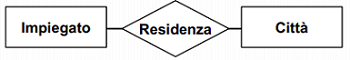
\includegraphics[scale=.61]{images/6.PNG}
\end{center}
\begin{center}
	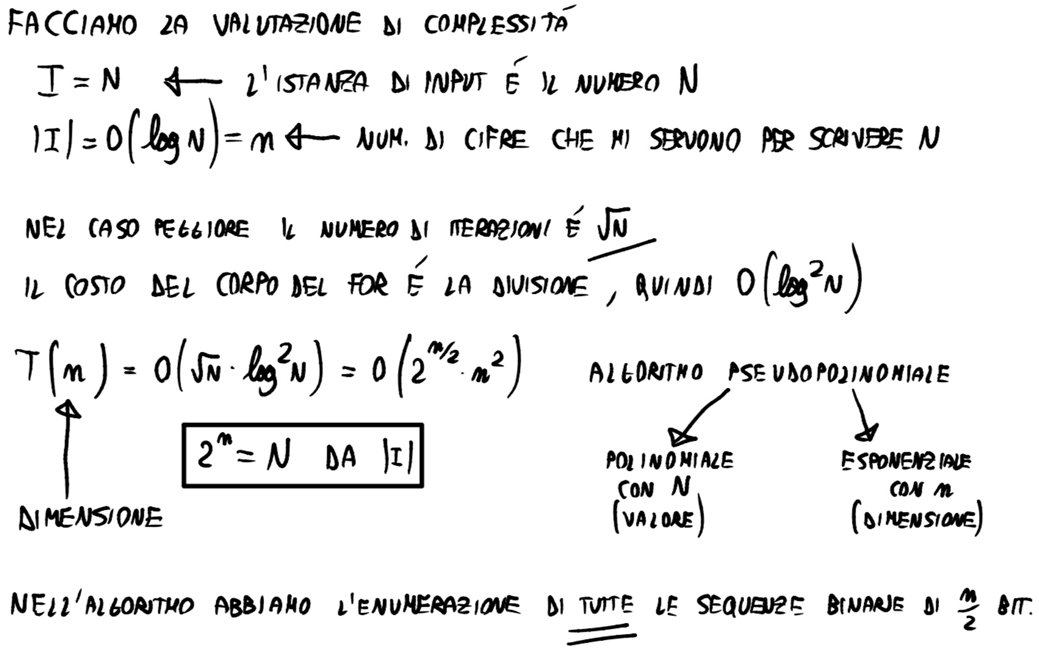
\includegraphics[scale=.7]{images/6bis.PNG}
\end{center}
L'algoritmo è pseudopolinomiale, cioè:
\begin{itemize}
	\item polinomiale rispetto al valore;
	\item \underline{esponenziale rispetto alla dimensione del valore} (non tengo conto solo del numero, ma anche di quanto è grande il numero).
\end{itemize}
Vogliamo un algoritmo più efficiente: introduciamo per questo il test di primalità secondo Miller-Rabin, basato su sequenze casuali.

\section{Test di primalità: algoritmo di Miller-Rabin}
\subsection{Premessa}
Vogliamo testare un intero dispari $N$ su $n$ bit. Se $N$ è dispari allora $N-1$ è pari.
$$
N-1 = 2^{\omega}z
$$
con $z$ dispari e $2^{\omega}$ la più grande potenza di $2$ che divide $N-1$. Vediamo due esempi:
\begin{align*}
	N &= 17 \implies N-1 = 16 = 2^{4} \cdot 1 \Longrightarrow z=1,\omega=4\\
	N &= 21 \implies N-1 = 20 = 2^{2} \cdot 5 \Longrightarrow z=5, \omega =2
\end{align*}
$z$ e $\omega$ ci serviranno nell'algoritmo: si noti che entrambi possono essere trovati in tempo polinomiale in quanto posso dividere un numero per $2$ al massimo $\log_2N$ volte quindi abbiamo un algoritmo polinomiale nel numero di cifre di $N$ ($n = \log_2N$)

\subsection{CN (ma non sufficienti) per il test di primalità} Supponiamo che $N$ sia un numero primo. Si prenda $y$, un intero casuale arbitrario tale che $ 2 \leq y \leq N-1 $ (che prende il nome di \emph{testimone}). Affermiamo che per $N$ valgono le seguenti proposizioni:
\begin{align*}
	\text{P1}:&\text{ } \text{MCD}(N, y) = 1\\\text{P2}:&\text{ } \left(y^z \text{ mod } N = 1\right) \text{ OR } \left(\exists i: 0 \leq i \leq \omega - 1 \text{ t.c. } y^{2^i \cdot z} \text{ mod } N = -1\right)
\end{align*}
Se il numero è primo allora vale sia P1 che P2. In P2 basta che una delle condizioni sia valida. Possiamo usare la veridicità di entrambi i predicati come condizione necessaria per il nostro test di primalità, tuttavia non è sufficiente in quanto esistono numeri composti (pochi) che verificano entrambi i predicati.

\subsection{Lemma di Miller-Rabin (pochi composti verificano le CN)}
Se $N$ è numero composto il numero di testimoni $y$ t.c. $2 \leq y \leq N-1$ che soddisfa i predicati $P1$ e $P2$ è basso, precisamente $< \frac{N}{4}$.
\paragraph{Cioè} Questo significa che se scelgo a caso un testimone $y$ la probabilità che ne scelga uno che rende veri i due predicati è minore della probabilità di scegliere un testimone dove uno dei due predicati è falso.
$$
    \text{P(scegliere $y$ t.c. $P1 \text{ AND } P2 = 1$)} < \frac{\frac{N}{4}}{N-2} < \frac{1}{4}
$$
Facciamo il rapporto tra casi favorevoli e casi possibile: $N-2$ è il numero di casi possibili (scelte possibili tra i testimoni), $\frac{N}{4}$ sono i casi favorevoli (in cui i due predicati sono entrambi soddisfatti).
\paragraph{Quindi} Immaginiamo i seguenti passi per verificare P1 e P2:
\begin{verbatim}
dato N scelgo a caso y in [2, N-1]
allora:
se uno dei due predicati è falso:
    N è certamente composto
se entrambi i predicati sono veri:
    N è composto con probabilità < 1/4, N è primo con probabilità > 3/4
\end{verbatim}
Per ridurre la probabilità posso re-iterare il processo di selezione di $y$. Se ripeto il procedimento $k$ volte scendiamo ad una probabilità 
$ < \frac{1}{4^k} $ che $N$ sia composto. Per avere un'idea  iteriamo il processo trenta volte:
\[k=30 \Longrightarrow \left(\frac{1}{4}\right)^{30} \simeq 10^{-18}\]


\subsection{Algoritmo completo e costo computazionale} 
Scriviamo l'algoritmo completo in pseudo-codice:
\begin{verbatim}
// Controlla la validita' del certificato y (certificato di N composto)
VERIFICA(N, y){
    if (P1 == false OR P2 == false) return 1
    return 0
}
TESTMR(N, k){
    for(i = 0; i < k; i++){
        y = numero a caso in [2, N-1]
        if(verifica(N, y) == 1) return 0    // N sicuramente non è primo
    }
    return 1            // N è primo con probabilità < 1/4^k
}
\end{verbatim}
\begin{itemize}
	\item Il costo di $\text{TESTMR}$ è $k \cdot \text{VERIFICA}$ in quanto si itera la verifica sul singolo testimone per k volte. L'esecuzione $k$ volte riduce la probabilità di errore da $\frac{1}{4}$ a $\left(\frac{1}{4}\right)^k$
	\item \textbf{Calcoli per il primo predicato}. La verifica di $P1$ è il calcolo del $MCD$ quindi si ha costo polinomiale nella dimensione di $N$ tramite l'algoritmo di Euclide.
	\begin{align*}
 		\text{ } \text{MCD}(N, y) = 1
	\end{align*}
	\item \textbf{Calcoli per il secondo predicato}. La verifica di $P2$ richiede il calcolo di potenze
	\begin{align*}\text{ } \left(y^z \text{ mod } N = 1\right) \text{ OR } \left(\exists i: 0 \leq i \leq \omega - 1 \text{ t.c. } y^{2^i \cdot z} \text{ mod } N = -1\right)
	\end{align*}
	La cosa è abbastanza critica perché queste operazioni richiedono tempo esponenziale nella dimensione di $N$. Si pensi che il valore massimo assumibile dall'esponente della $y$ si ha con $i=\omega - 1$, quindi risulta necessario fare $\frac{N-1}{2}$ moltiplicazioni (otteniamo ciò da $N-1=2^\omega z$, la premessa poco avanti) per ottenere il risultato desiderato \[2^{(\omega-1)} \cdot z=\frac{N-1}{2} \Longrightarrow \text{Caso peggiore: } y^{2^{(\omega-1)} \cdot z} = y^{\frac{N-1}{2}} \]
	
	Risolviamo il problema implementando l'\textbf{algoritmo delle quadrature successive} (posto nell'appendice sull'algebra modulare), con cui riduciamo il numero di moltiplicazioni richieste per ottenere una potenza.
\end{itemize}

\clearpage 

\section{Generazione di numeri primi}
\begin{framed}
	\noindent \textbf{Domanda da esame}.
	
	\noindent Illustrare con quale metodo si generano numeri primi grandi in crittografia e spiegare perché tale 	metodo è considerato efficiente.
\end{framed}
Non abbiamo algoritmi propri per la generazione di numeri primi però possiamo seguire il seguente approccio:
\begin{enumerate}
    \item generare un numero casuale
    \item si testa la sua primalità
    \item se questo numero casuale non è \emph{dichiarato} primo si aumenta di due e si ripete da (2)
\end{enumerate}
\paragraph{Densità dei numeri primi sull'asse degli interi} L'algoritmo introdotto conviene perché per un lemma di Gauss sappiamo che il numero di interi primi e minori di un numero dato $N$ tende a:
$$ \longrightarrow{} \frac{N}{\log_eN} \,\,\,\,\text{per }N \to \infty$$
quindi preso un $N$ abbastanza grande sappiamo con quasi certezza che esisterà un primo in un intorno circolare di ampiezza $\log_eN$.

\paragraph{Algoritmo} Scriviamo quindi un algoritmo in pseudocodice:
\begin{verbatim}
PRIMO(n): // n : numero di bit desiderati per il numero primo
    S = sequenza casuale di n-2 bit
    N = 1 S 1 // concatenamento dei bit per avere num. lunghi e sicuramente dispari
    while(TESTMR(N, K) == 0) N += 2
    return N
\end{verbatim}
L'1 come bit più significativo serve per avere un numero sempre elevato (potrei avere sequenze con bit più significativi tutti uguali a 0), l'1 meno significativo mi da certezza che andremo a considerare un numero dispari. Abbiamo quindi TESTMR con complessità O($n^3$), viene ripetuto O($n$) volte quindi in totale l'algoritmo ha complessità: O($n^4$). 



	\part{Cifrari storici}
\chapter{Introduzione}
I cifrari sono nati per comunicazioni "sicure" ristrette a poche persone: la cosa si contrappone alla crittografia moderna e di massa, dove la sicurezza non è più legata alla non conoscenza dell'algoritmo da parte del crittoanalista. (quindi in piena contrapposizione alla crittografia moderna di massa). Distinguiamo i seguenti tipi di cifrari:
\begin{itemize}
	\item cifrari a sostituzione, che possono essere monoalfabetici o polialfabetici;
	\item cifrari a trasposizione.
\end{itemize}
Vedremo alla fine la crittoanalisi statistica, utilizzata per forzare questi cifrari.
\section{Principi di Ruggero Bacone} 
Tutti i cifrari storici rispettano i principi di \emph{Ruggero Bacone} che dicono:
\begin{itemize}
    \item cifratura e decifratura (funzioni C e D) devono essere eseguibili facilmente;
    \item deve essere impossibile decifrare il messaggio senza conoscere l'algoritmo (non posso ricavare la funzione D se la funzione C non è nota);
    \item il crittogramma deve apparire innocente (non deve destare sospetto, deve sembrare un messaggio in chiaro).
\end{itemize}

\chapter{Cifrari a sostituzione}
\section{Tipologie}
I cifrari a sostituzione si dividono in due classi:
\begin{itemize}
	\item \textbf{monoalfabetici}, un carattere si sostituisce sempre con lo stesso carattere (per esempio il cifrario di Cesare);
	\begin{itemize}
		\item Possibile impiegare funzioni di cifratura e decifrazione più complesse dell'addizione e della sottrazione in modulo.
		\item Lo spazio delle chiavi è molto più ampio.
		\item La sicurezza è comunque molto modesta.
	\end{itemize} 
	\item \textbf{polialfabetici}, un carattere si sostituisce con una lettera scelta da un insieme di lettere possibili, secondo una qualche regola (a seconda del contesto in cui appare la lettera).
\end{itemize}
\section{Cifrario monoalfabetico: \emph{cifrario di Cesare}}
Il cifrario di Cesare è il primo di concezione moderna, tuttavia è senza chiave. La sua sicurezza si basa sulla ristrettezza di chi lo conosce. Si può generalizzare scegliendo un $k$ arbitrario che indica di quanti posti dobbiamo ruotare l'alfabeto. Supponiamo $k=3$, otteniamo
\begin{center}
	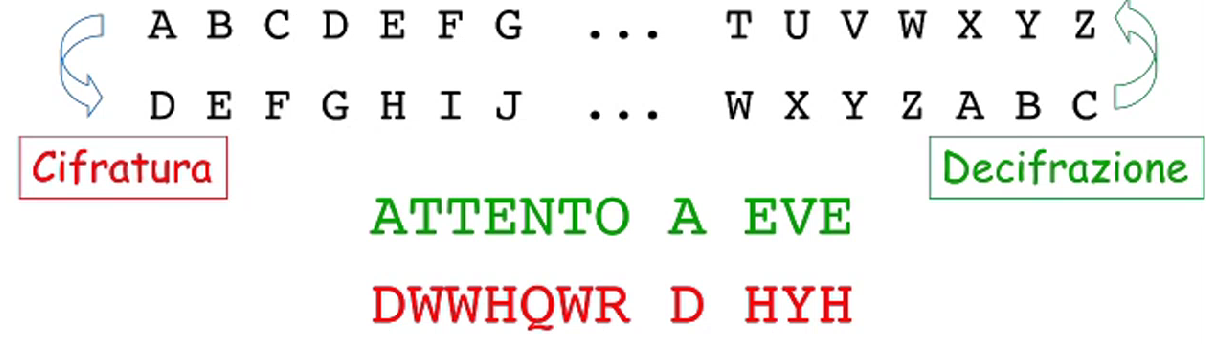
\includegraphics[scale=.45]{images/7.PNG}
\end{center}
Si legge da sopra a sotto per cifrare, da sotto a sopra per decifrare. 
\paragraph{Rafforzamento del cifrario} Possiamo rafforzare il cifrario ponendo $k$ come chiave: i due interlocutori decidono un valore $1 \leq k \leq 25$ (non $26$, altrimenti il messaggio risultante è lo stesso posto in input).
\paragraph{Generalizzazione} Indichiamo con $pos(x)$ la posizione di $x$ nell'alfabeto
\[\text{pos}(A)=0,\dots,\text{pos}(Z)=25\]
per cifrare si deve quindi sostituire $x$ con:
$$ y : \text{pos}(y) = \left(\text{pos}(x) + k\right) \text{ mod } 26 $$
dove $k$ è la chiave, $1\leq k \leq 25$. Per decifrare si sostituisce $y$ con:
$$ x : \text{pos}(x) = \left(\text{pos}(y) - k\right) \text{ mod } 26 $$Si può forzare facilmente (con attacco forza bruta) in quanto le chiavi sono poche. 
%\paragraph{Cifrario di sostituzione} Questo cifrario appartiene alla classe dei \emph{cifrari a sostituzione} cioè quelli in cui ogni lettera viene scambiata con un'altra o più di una seguendo un determinato ordine.
\paragraph{Esempio} Prendiamo $k=10$. Vogliamo cifrare $R$
\[\text{pos}(R)=17 \Longrightarrow (17+10)\,\text{mod}\,26=1=\text{pos}(B)\]
\begin{framed}
 \noindent \textbf{Esercizio da esame}, Decifrare il seguente crittogramma
	\begin{verbatim}YMNXJCJWHNXJNXJFXD\end{verbatim}
Deve essere trovata la chiave, facendo prove si trova che $k=5$ (ho usato un sito online)
\begin{verbatim}
	YMNXJCJWHNXJNXJFXD -> THISEXERCISEISEASY
\end{verbatim}
\end{framed}
\paragraph{Proprietà commutativa del cifrario} 
Questo cifrario gode della proprietà commutativa, cioè data una sequenza di chiavi e di cifrature cambiando l'ordine in cui le eseguiamo non si varia il crittogramma finale. Questo significa che
\begin{align*}
	C(C(s, k_2), k_1) = C(s, k_1 + k_2)\\
	D(D(s, k_2), k_1) = D(s, k_1 + k_2)
\end{align*}
Comporre più cifrature non aumenta la sicurezza del sistema!



\section{Cifrario monoalfabetico: \emph{cifrario affine}}
Una lettera in chiaro $x$ viene sostituita con la lettera cifrata $y$ che occupa nell'alfabeto la seguente posizione:
$$x: \text{pos}\left(y\right) = \left(a \cdot \text{pos}\left(x\right) + b\right)\text{ mod } 26 $$
Abbiamo come chiave segreta del cifrario $K = <a, b>$. Mentre la cifratura rimane cosa semplice la decifrazione diventa più complessa. 
$$ y \xrightarrow{} x : pos\left(x\right) = a^{-1} \cdot (pos\left(y\right) - b) \text{ mod } 26 $$
dove $a^{-1}$ è l'inverso di $a\,\text{mod}\,26$. Per maggiore chiarezza si invita a leggere le nozioni di algebra modulare.
%con $a \cdot a^{-1} \mod 26 = 1$. 
\paragraph{Scelta della chiave} Per far funzionare la decriptazione $a$ e $b$ vanno scelti in maniera particolare:
\begin{itemize}
	\item $b$ si può scegliere a piacere
    \item $a$ va scelto invertibile cioè deve esistere...
    \[a^{-1} : a \cdot a^{-1} \,\text{mod}\, 26 = 1\]
    Generalizzando affermiamo che l'inverso di un intero $a$ modulo $m$ esiste ed è unico \emph{se e solo se i due numeri sono coprimi}, cioè $\text{MCD}(a, 26) = 1$. Se il MCD è diverso da $1$ allora non si ha l'iniettività e non è possibile decifrare. Si veda il teorema dell'inverso nelle nozioni di algebra modulare per capire il perchè.
\end{itemize}
%Scegliendo $a$ primo si vince sempre!
\paragraph{Esempio funzionante} $K=<3,1>$
$$\text{IL NOSTRO TEMPO} \Longrightarrow \text{ZI OREGAR GNBUR}$$
La chiave è valida poichè $\text{MCD}(3,26)=1$. Il fatto che $3$ e $26$ siano coprimi garantisce l'esistenza dell'inverso.
\paragraph{Esempio non funzionante} $$K = <13, 0>$$
La chiave non è valida poichè $\text{MCD}(13,26) \neq 1$.
\begin{itemize}
	\item Tutte le lettere in posizione pari vengono trasformate in $A: \text{pos}(A)=0$
	\begin{align*}
		A &\Longrightarrow \text{pos}(y) = (13 \cdot \text{pos}(A)+0) \text{ mod }26 = 0 \text{ mod } 26 =0\\
		C &\Longrightarrow \text{pos}(y) = (13 \cdot \text{pos}(C)+0) \text{ mod }26 = 13 \cdot 2 \text{ mod } 26 = 26 \text{ mod } 26 =0\\
		E &\Longrightarrow \text{pos}(y) = (13 \cdot \text{pos}(E)+0) \text{ mod }26 = 13 \cdot 4 \text{ mod } 26 = 52 \text{ mod } 26 =0\\
		G &\Longrightarrow \text{pos}(y) = (13 \cdot \text{pos}(G)+0) \text{ mod }26 = 13 \cdot 6 \text{ mod } 26 = 78 \text{ mod } 26 =0
	\end{align*}
	\item Tutte le lettere in posizioni dispari vengono trasformate in $B: \text{pos}(B)=13$
	\begin{align*}
		B &\Longrightarrow \text{pos}(y) = (13 \cdot \text{pos}(B)+0) \text{ mod }26 = 13 \text{ mod } 26 =13\\
		D &\Longrightarrow \text{pos}(y) = (13 \cdot \text{pos}(D)+0) \text{ mod }26 = 13 \cdot 3 \text{ mod } 26 = 39 \text{ mod } 26 =13\\
		F &\Longrightarrow \text{pos}(y) = (13 \cdot \text{pos}(F)+0) \text{ mod }26 = 13 \cdot 5 \text{ mod } 26 = 65 \text{ mod } 26 =13\\
		H &\Longrightarrow \text{pos}(y) = (13 \cdot \text{pos}(H)+0) \text{ mod }26 = 13 \cdot 7 \text{ mod } 26 = 91 \text{ mod } 26 =13
	\end{align*}
\end{itemize}
\paragraph{Numero di chiavi} Proviamo a contare le possibili chiavi tale che $a$ e 26 siano coprimi. I fattori primi di 26 sono $2$ e $13$:
$$ 26 = 2 \cdot 13 $$
Escludiamo i numeri pari (26 multiplo di 2) e 13 (non i multipli visto che non ci sono, agiamo modulo 26): il numero di valori assumibili da $a$ è il seguente.
$$ a \in \{ \text{Numeri dispari tra 1 e 25 tranne 13} \} \xrightarrow{} 12 \text{ valori possibili} $$
Mentre $b$ può essere scelto con maggiore libertà, tenendo conto di un solo criterio:
$$ \text{b scelto a piacere tra 0 e 25} \xrightarrow{} 26 \text{ valori possibili } $$
Se le chiavi legittime sono le coppie $<a,b$ allora abbiamo $12 \times 26 = 312$ chiavi (in realtà $311$ visto che la coppia $<1,0>$ lascia inalterato il messaggio). 
\paragraph{Segretezza della chiave} Le chiavi sono troppo poche. Se la segretezza dipende unicamente dalla chiave allora \textbf{il numero delle chiavi deve essere così grande da essere immune da tentativi di ricerca esaustiva} e poi va scelto in maniera casuale. Come possiamo fare ciò in un cifrario monoalfabetico? Col prossimo cifrario.


\section{Cifrario monoalfabetico: \emph{cifrario completo}}
Generiamo una permutazione a caso dell'alfabeto e la usiamo come chiave.
$$ \text{Lettera in chiaro di posizione i} \Longrightarrow \text{Lettera di posizione i nella permutazione} $$
\small 
\begin{align*}
	A&&B&&C&&D&&E&&F&&G&&H&&I&&J&&K&&L&&M&&N&&O&&P&&Q&&R&&S&&T&&U&&V&&W&&X&&Y&&Z\\
	S&&D&&T&&K&&B&&J&&O&&H&&R&&Z&&C&&U&&N&&Y&&E&&P&&X&&V&&F&&W&&A&&G&&Q&&I&&L&&M
\end{align*}
\normalsize 
\paragraph{Quante possibili chiavi ci sono?} Una chiave è una permutazione di 26 lettere, quindi lo spazio è $26! - 1 \text{ } (~4 \cdot 10^{26})$. Nel calcolo leviamo $1$ per non considerare una corrispondenza dove nessun carattere risulta alterato.
\paragraph{Problema risolto?} Questo grande spazio di chiavi tuttavia non è sufficiente a dire che il sistema è sicuro in quanto rimangono vulnerabilità basate su:
\begin{itemize}
    \item strutture logiche dei messaggi in chiaro;
    \item occorrenza statistica delle lettere (osserviamo la lettera più frequente nel messaggio cifrato, questa potrebbe corrispondere alla lettera usata più frequentemente nell'alfabeto italiano).
\end{itemize}
Queste cose sono risolvibili solo passando ai cifrari polialfabetici. 

\section{Cifrario polialfabetico: archivio fotografico di Augusto}
Il cifrario non veniva usato per comunicare ma per mantenere un archivio di informazioni cifrato. Esso fu svelato a seguito della sua morte dall'imperatore Claudio:
\begin{itemize}
    \item Augusto scriveva i messaggi in greco, poi metteva in corrispondenza la sequenza di lettere del documento con la sequenza di lettere del primo libro dell'Iliade;
    \item sostituiva ogni lettera del documento con il numero che indicava la distanza tra le due lettere (quella nel messaggio in chiaro e quella nel primo libro dell'Iliade) nell'alfabeto greco.
\end{itemize}
\paragraph{Esempio}
\begin{itemize}
	\item \textbf{Lettera in posizione $i$ nel documento}: $\alpha$
	\item \textbf{Lettera in posizione $i$ nell'Iliade}: $\epsilon$
	\item \textbf{Carattere in posizione $i$ nel crittogramma}: $4$ (distanza tra $\alpha$ ed $\epsilon$).
\end{itemize}
\paragraph{Forzatura} Il cifrario è stato forzato perché Claudio ha trovato il libro dell'Iliade di Augusto con scritture, calcoli ed annotazioni. Il cifrario aumenta in sicurezza cambiando la pagina del libro ogni volta che si cripta un nuovo documento.
\paragraph{Perchè polialfabetico?} Il cifrario è polialfabetico poichè tutte le $\alpha$, ad esempio, non vengono sostituite sempre dal solito carattere. Dipende dalla posizione $i-$esima nel documento (nel caso di Augusto il primo libro dell'Iliade).

\section{Cifrario polialfabetico: disco dell'Alberti (XV secolo)}
Abbiamo due dischi ruotanti:
\begin{itemize}
	\item quello esterno ha lettere (italiane) e numeri, e si usa per formulare il messaggio
	\item quello interno, più ricco (alfabeto inglese), ha lettere disposte in maniera arbitraria e diversa per ogni coppia di utenti
\end{itemize}
Ruotando uno dei due dischi è possibile ottenere corrispondenze diverse.
\begin{center}
	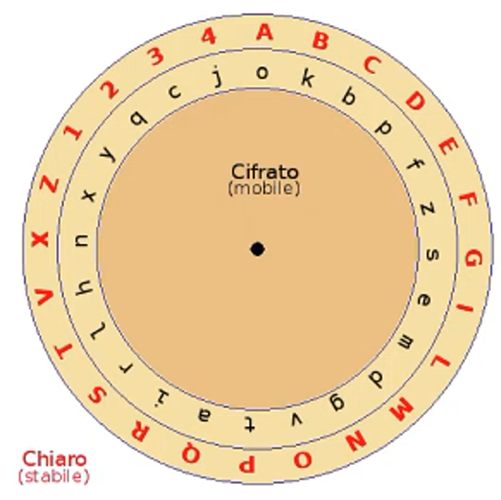
\includegraphics[scale=.45]{images/8.PNG}
\end{center}
\subsection{Primo metodo di cifratura} I dischi sono disposti in modo da ottenere la corrispondenza seguente...
\begin{verbatim}
ABCDEFGHILMNOPQRSTUVZ12345 <-- CHIAVE A-S
SDTKBJOHRZCUNYEPXVFWAGQILM

ABCDEFGHILMNOPQRSTUVZ12345 <-- CHIAVE A-Q
QILMSDTKBJOHRZCUNYEPXVFWAG

Chiave iniziale: A-S
messaggio: NON FIDARTI DI EVE
m = NONFIDA 2 RTIDIEVE
c = UNUJRKS Q UYBMBSPS
quando si arriva su 2 la chiave diventa A-Q
\end{verbatim}
Inizialmente abbiamo la chiave A-S, cioè indichiamo che tra i due dischi si debba avere corrispondenza tra A esterno ed S interno. Il numero due costituisce un carattere speciale, che determina un cambio di chiave: quando si arriva alla lettera Q si nota la corrispondenza con 2 e la chiave diventa A-Q (primo carattere con cui stabilisco la corrispondenza è sempre $A$, il secondo è quello che si trova nella corrispondenza con $2$).

\subsection{Secondo metodo di cifratura} C'è un secondo modo per usare questi dischi: il metodo dell' \emph{indice mobile}:
\begin{verbatim}
ABCDEFGHILMNOPQRSTUVZ12345 <-- CHIAVE A-E
EQHCWLMVPDNXAOGYIBZRJTSKUF

ABCDEFGHILMNOPQRSTUVZ12345 <-- CHIAVE A-P
PDNXAOGYIBZRJTSKUFEQHCWLMV

m: ILD 2 EL P FINO
c: PDC S WD O OIRJ
\end{verbatim}
Inizialmente la chiave è A-E, poi decifrando si trova 2: tra due lettere si cambia chiave. Si decifrano quindi altre 2 lettere nella giusta maniera e la lettera dopo sarà P cioè la nuova chiave A-P e successivamente si inizia a decifrare con questa nuova chiave. In genere si cambia chiave ogni volta che si trova un carattere speciale. Con caratteri speciali frequenti il cifrario è difficle da attaccare, poichè la chiave viene alterata ad intervalli imprevedibili.
\clearpage 

\section{Cifrario polialfabetico: De Vigenère}
\begin{framed}
\noindent \textbf{Esercizio da esame}.\\
Esporre come funziona il cifrario di de Vigenère e descrivere il principale attacco che può essere
condotto contro di esso.
\end{framed} 
E' una estensione della tecnica dell'Alberti più sicura che è rimasta irrompibile per 3 secoli. Si sceglie una chiave in cui ogni lettera corrisponde ad un numero che sarà di quanto bisogna shiftare il testo in chiaro per ottenere il testo cifrato:
\begin{table}[ht!]
    \centering
    \begin{tabular}{c c c c c c}
        C & H & I & A & V & E \\
        2 & 7 & 8 & 0 & 24 & 4
    \end{tabular}
\end{table}
la chiave si ripete tante volte quanto serve per equiparare il messaggio in lunghezza (nel caso in cui la lunghezza della chiave sia più piccola del messaggio da cifrare):
\begin{center}
	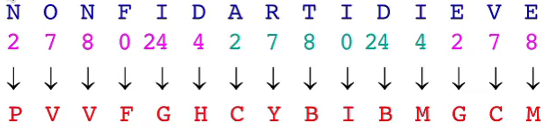
\includegraphics{images/9.PNG}
\end{center}

\paragraph{Rappresentazione alternativa con matrice} Si può vedere anche con una matrice 26x26 in cui ad ogni incrocio si trova la lettera $i$ criptata con la lettera $j$. In sostanza indichiamo nella matrice non i numeri rappresentanti le traslazioni, ma direttamente i caratteri.

\paragraph{Sicurezza della chiave} La sicurezza di questo metodo è influenzata dalla lunghezza della chiave: se la chiave è di piccola dimensione allora il numero di volte in cui si manifestano certa traslazioni aumenta. Addirittura, ponendo la chiave con dimensione $h=1$ ottengo l'equivalente del cifrario monoalfabetico di Cesare. Maggiore è la lunghezza della chiave, maggiore è la sicurezza.
\begin{itemize}
	\item \textbf{Idea di attacco}.
	
	Supponiamo di conoscere la lunghezza $h$ della chiave; costruiamo dei sottomessaggi formati dalle lettere che occupano tutte le stesse posizioni mod $h$. In ciascuno di questi messaggi tutte le lettere sono allineate alla stessa lettera della chiave quindi è come se fossero cifrate con un metodo monoalfabetico.
	
	\item \textbf{Sicurezza a confronto coi cifrari monoalfabetici}.
	
	I cifrari polialfabetici non sono molto più sicuri dei metodi monoalfabetici se le chiavi sono piccole! Se la chiave è lunga quanto il messaggio, è casuale e non riutilizzata otteniamo un cifrario \emph{perfetto} (ovviamente aumenta la difficoltà d'uso). E' il caso del \emph{one-time-pad} che usa una codifica binaria (1917).
\end{itemize}
\clearpage 

\chapter{Cifrari a trasposizione}
In questi cifrari non sostituiamo lettere come fatto fino ad ora. Il crittogramma presenta le seguenti caratteristica:
\begin{itemize}
	\item è una permutazione dei caratteri del mess aggio originario;
	\item in alcuni casi può includere lettere aggiuntive, ignorate nella decifrazione.
\end{itemize}

\section{Cifrario a permutazione semplice} 
La chiave consiste nella coppia $<h, \Pi>$. 
\begin{itemize}
	\item Dividiamo il messaggio da cifrare in blocchi aventi lunghezza $h$. Nel caso in cui il numero di caratteri che costituiscono il messaggio non sia multiplo di $h$ andremo ad aggiungere nell'ultimo blocco dei \emph{caratteri padding}, in modo che tutti i blocchi siano di dimensione $h$.
	\item Definiamo un insieme di posizioni $\Pi$, con cui rappresento una permutazione degli interi $\{1,\dots,h\}$ (ovviamente ho un numero di interi pari a $h$).
\end{itemize}
Vediamo col seguente esempio.
\paragraph{Esempio} $h = 9, \Pi=\{1, 2, 5, 3, 7, 6, 4, 9, 8\}$
\begin{center}
	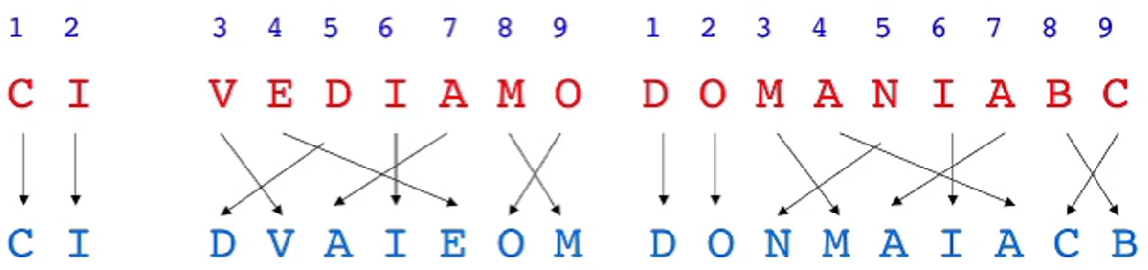
\includegraphics[scale=.5]{images/10.PNG}
\end{center}
\paragraph{Numero di chiavi possibili} Le chiavi sono le possibili permutazioni: $h!-1$. Non si considera quella che lascia invariato il messaggio.
\section{Cifrario a permutazione di colonne}
La chiave consiste nella terna $k=<c, r, \Pi>$
\begin{itemize}
	\item $c$ ed $r$ sono il numero di colonne e righe di un tavolo da lavoro $T$ dove andremo a collocare il messaggio in chiaro (di fatto il tavolo da lavoro è una matrice di $r$ righe e $c$ colonne).
	\item $\Pi$ è la permutazione degli elementi $\{1, 2, \dots, c\}$. Ciò che andremo a spostare non sono caratteri, ma colonne del tavolo $T$!
\end{itemize}
Si prende il messaggio e lo si decompone in blocchi $m_1, m_2, \dots$ di $c \times r$ caratteri ciascuno, eventualmente aggiungendo \textit{padding}. I caratteri si distribuiscono tra le celle della matrice $T$, riempiendo le righe dall'alto verso il basso. Si veda il seguente esempio.

\paragraph{Esempio} Vogliamo cifrare la frase \emph{NON SONO IL COLPEVOLE}.
$$c = 6, r = 3, \Pi=\{2, 1, 5, 3, 4, 6\}$$
\begin{center}
	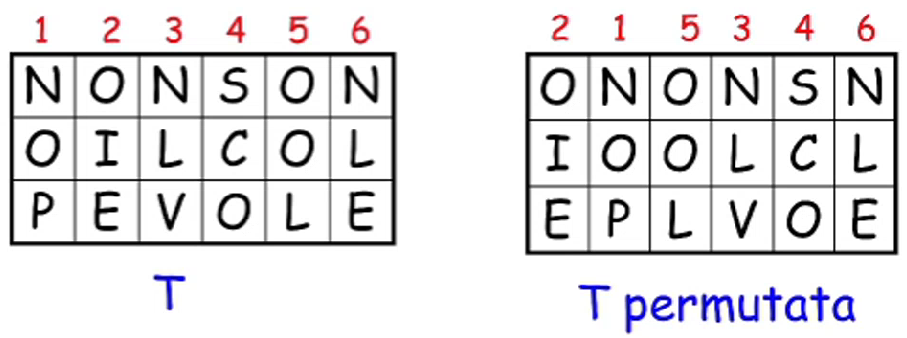
\includegraphics[scale=.4]{images/11.PNG}
\end{center}
Dalla lettura per colonne otteniamo il crittogramma \textit{OIENOPOOLNLVSCONLE}. In questo caso facciamo tutto in un unico blocco. Le chiavi sono esponenziali non avendo un tetto massimo per $r$ e $c$.


\section{Cifrario a griglia (\emph{cifrario di Richelieu})}
\begin{framed}
	\noindent \textbf{Domanda da esame}.\\Spiegare cosa s’intende per cifrario (storico) a griglia, indicare come si costruisce una griglia e
	quante griglie diverse si possono costruire per ogni dimensione scelta.
\end{framed} 
\paragraph{Versione innocente}
Un esempio è il cifrario di \emph{Richeliu}: il crittogramma è celato in un libro, la chiave è una scheda perforata e la pagina di un libro. Facendo corrispondere la scheda con la pagina si vedono le lettere che compongono il messaggio. Il fatto che si prenda la pagina di un libro garantisce il rispetto del principio di innocenza di Bacone. 
\paragraph{Versione non innocente} Rinunciando al principio di innocenza usiamo una griglia quadrata $q\times q$ con $q$ pari, $s = \frac{q^2}{4}$ è il numero delle celle trasparenti che compongono il messaggio. Si scrivono i primi $s$ caratteri del messaggio nelle posizioni corrispondenti alle celle trasparenti. La griglia viene ruotata tre volte di $90$° in senso orario e si ripete per ogni rotazione l'operazione di scrittura dei 3 gruppi successivi si $s$ caratteri.

\paragraph{Esempio} Vogliamo cifrare la frase \emph{L'ASSASSINO E' ARCHIMEDES TARRINGTON}.
\begin{center}
	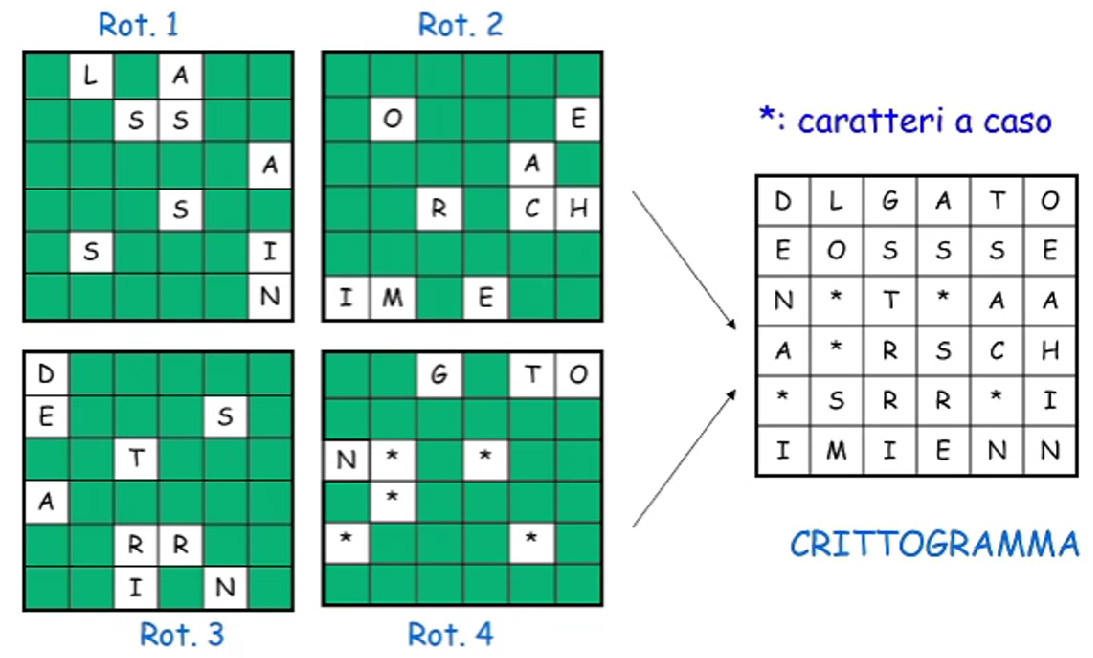
\includegraphics[scale=.38]{images/12.PNG}
\end{center}
Abbiamo $q=6, s=\frac{6^2}{4}=9$. La griglia va costruita in modo che una cella già usata non ricapiti nuovamente. Se la lunghezza è maggiore di $4s$ si riempiono più tabelle. La decifrazione si ottiene applicando la maschera e leggendo. 

\paragraph{Griglie possibili} Le griglie possibili sono $G = 4^s = 4^{\frac{q^2}{4}}$. Per $q=6$ otteniamo
$$G = 4^9 \approx 260'000$$Si arriva a questo numero perché:
\begin{itemize}
    \item immaginiamo di dover creare la maschera, scegliamo il primo foro e dobbiamo sceglierlo in modo che ruotando la griglia non sia nuovamente scoperto.
    \item si devono scegliere $s$ buchi, per ogni cella se ne deve scegliere una su 4 quindi $4^s$ chiavi possibili
\end{itemize}
\clearpage 

\chapter{Forzatura dei cifrari storici}
\section{Crittoanalisi statistica}
\begin{framed}
	\noindent \textbf{Domanda da esame}.\\Spiegare cosa s’intende per crittoanalisi statistica e come essa possa essere impiegata nell’attacco ai
	cifrari a sostituzione monoalfabetica e polialfabetica.
\end{framed} 
Abbiamo detto che la sicurezza di un cifrario dipende dalla dimensione delle chiavi, in modo tale da impedire la forzatura del cifrario stesso attraverso ricerche esaustive. Fino ad ora abbiamo pensato a forzature del cifrario con individuazione di chiave, ma il metodo non è l'unico possibile.  I cifrari storici, in particolare, sono stati violati con un attacco statistico di tipo \emph{cipher-text} (si conosce solo il crittogramma). 
\paragraph{Ipotesi} Il metodo si afferma in Europa nel XIX secolo con la forzatura del cifrario di Vigenère. Si fanno delle ipotesi:
\begin{itemize}
    \item si suppone di conoscere il metodo di cifratura/decifratura (si da per scontato che il crittoanalista conosca il metodo);
    \item si suppone che il crittoanalista conosca il messaggio naturale in cui sono scritti i messaggi;
    \item si suppone di avere messaggi abbastanza lunghi da far valere le statistiche note dei linguaggi naturali.
\end{itemize}
\begin{center}
	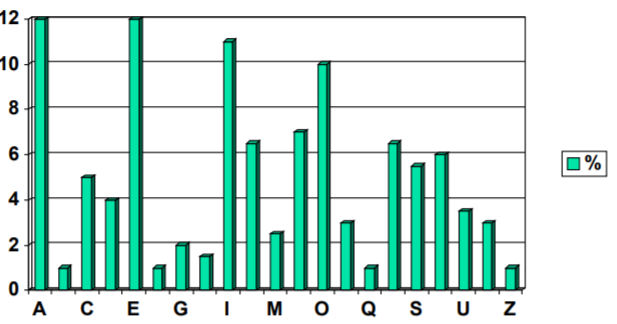
\includegraphics[scale=.56]{images/13.PNG}
\end{center}
La frequenza con cui appaiono le lettere dell'alfabeto è ben studiata in ogni lingua così come sono note le frequenze dei \emph{digrammi}, \emph{trigrammi}, \emph{q-grammi} (gruppi da 2, 3, $q$ lettere). Nell'italiano le lettere A ed E costituiscono il 12\% dei messaggi. Si calcola il grafico delle frequenze dei caratteri all'interno del crittogramma: se siamo davanti ad un cifrario a sostituzione monoalfabetico avremo un grafico che è permutazione del grafico delle frequenze italiane, possiamo quindi dire che è molto probabile che se $$\text{freq}\left(x\right) \approx \text{freq}\left(y\right)$$ allora $x$ è stato criptato con $y$.
%\paragraph{Istogramma delle frequenze} In genere l'istogramma delle frequenze è utile per individuare la tipologia di cifrario adottato.
%\begin{itemize}
%	\item \textbf{Trasposizione}: grafico pressochè identico a quello del linguaggio
%	\item \textbf{Sostituzione monoalfabetica}: permutazione del grafico del linguaggio
%	\item \textbf{Sostituzione polialfabetica}: grafico è pressoché piatto
%\end{itemize}
\section{Cifrari a sostituzione monoalfabetici}
\begin{itemize}
	\item \textbf{Cifrario di Cesare}. 
	
	Nel caso del cifrario di Cesare abbiamo uno shift del grafico. Ci basta individuare una corrispondenza per trovare tutte le altre. 
	
	\begin{center}
		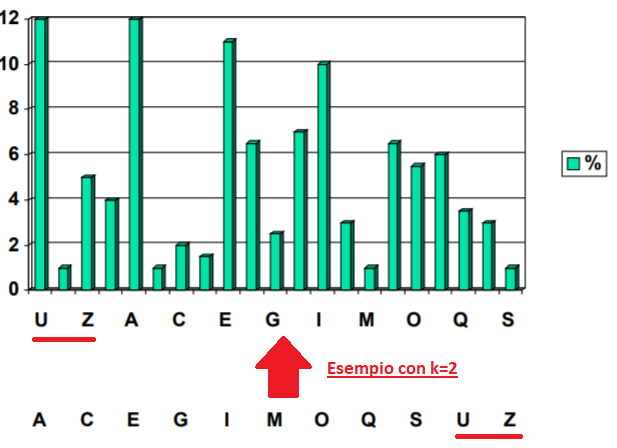
\includegraphics[scale=.55]{images/13bis.PNG}
	\end{center}

	L'attacco a forza bruta rimane la cosa più semplice, visto l'esiguo numero di chiavi. 
	
	\item \textbf{Cifrario affine}. 
	
	Nel caso di cifrari affini una volta trovate due lettere $a,b$ si imposta il sistema di equazioni e si risolve. Il cifrario è per definizione invertibile (basata avere $\text{MCD}(a,m)=1$, quindi $a,m$ coprimi), dunque la risoluzione del sistema è sempre possibile.
	\item \textbf{Cifrario completo}. 
	
	Nel caso di un cifrario completo (permutazione arbitraria) non abbiamo lo shift del grafico, ma una permutazione dove le frequenze non sono associate ai relativi caratteri. Quello che facciamo è associare le lettere del messaggio cifrato (l'unico che abbiamo) in base alle frequenze.
	
	\textbf{Esempio}: so che una lettera (o un insieme di lettere) è quella maggiormente utilizzata nella lingua italiana. Verifico nel cifrario quale carattere è stato utilizzato maggiormente: confrontando le frequenze potrei individuare una corrispondenza.
\end{itemize}
\clearpage 

\section{Cifrari a sostituzione polialfabetica} 
Nella sostituzione polialfabetica la decifrazione è più difficile! A una lettera possono corrispondere lettere diverse: l'istogramma delle frequenze è piatto.
\begin{itemize}
	\item \textbf{Cifrario dell'alberti}.
	
	Il cifrario dell'Alberti è immune da questi attacchi se la chiave viene cambiata spesso evitando \textit{pattern} ripetitivi. Mantenere la stessa chiave a lungo è come usare un cifrario monoalfabetico, precisamente un cifrario completo.
	
	\item \textbf{Cifrario di Vigenère}.
	\begin{itemize}
		\item La lettera $y$ non dipende solo dalla lettera del testo in chiaro, ma anche dalla lettera corrispondente della chiave.
		\item La chiave è spesso piccola e ripetuta più volte: se sappiamo che la chiave ha lunghezza $h$ possiamo raggruppare le lettere in posizioni $h,2h,3h,\dots$ e poi $h+1,2h+1,\dots$ e così via. In questo modo si ottengono $h$ gruppi cifrati in maniera monoalfabetica: se individuo una coppia allora individuo tutte le altre coppie del gruppo analizzato.
		\item Si deve stimare la lunghezza della chiave: si studiano i digrammi ed i trigrammi alla ricerca di sequenze che si ripetono nella speranza che lo stesso digramma/trigramma sia criptato allo stesso modo e si prende la loro distanza come multiplo della lunghezza della chiave (o la chiave stessa). E' molto più probabile che si generi in questo modo piuttosto che sia generato casualmente.
	\end{itemize}
\end{itemize}
\section{Cifrari a trasposizione}
Nei cifrari a trasposizione non ha senso calcolare l'istogramma delle frequenze in quanto il crittogramma è una permutazione delle lettere del testo in chiaro (le frequenze sono le stesse). In questi casi si usa lo studio dei q-grammi. In particolare se si sa la lunghezza $h$ della chiave:
\begin{itemize}
	\item si divide il crittogramma in blocchi di $h$ lettere
	\item in ciascun gruppo si cercano i gruppi di q lettere che formano i q-grammi più diffusi nel linguaggio
	\item se si trova un vero q-gramma si ottiene parte della chiave
\end{itemize}

\begin{framed}
	\noindent \textbf{Osservazione conclusiva}. 
	
	\noindent La crittoanalisi statistica permette di fare due cose:
	\begin{itemize}
		\item individuare il possibile cifrario adottato da chi ha generato il crittogramma;
		\item individuare (in alcuni casi) le corrispondenze, cioè decifrare in tutto o in parte il crittogramma.
	\end{itemize}
\end{framed} 

\chapter{La macchina Enigma}
Rappresenta l'ultimo esempio di cifrario storico, il primo che porta a dei sistemi automatizzati e gli sforzi fatti per rompere questo sistema sono stati importanti per l'evoluzione storica dell'informatica. Nasce in Germania nel 1918 ed è una modifica automatizzata del cifrario dell'Alberti.
\begin{center}
	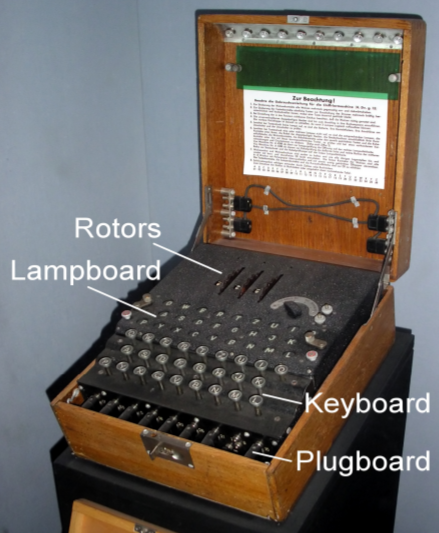
\includegraphics[scale=.55]{images/14.PNG}
\end{center}
Si compone di una tastiera di ventisei lettere (alfabeto tedesco) più altrettante lampadine rappresentanti lettere. Ogni volta che l'utente preme un tasto si illumina il corrispondente carattere del crittogramma. L'utente osserva la luce accesa, si segna la lettera e prosegue col carattere successivo. Lo stesso approccio vale per la decifrazione. Si osservi che nella cifratura premere più volte lo stesso carattere sulla tastiera porta ad ottenere un crittogramma costituito da caratteri diversi.
\section{Chiave e assetto iniziale} La chiave è l'assetto iniziale della macchina. Questo assetto rende reversibile la cifratura: un assetto permette di cifrare ($A \xrightarrow{} F$) ma anche di decifrare ($F \xrightarrow{} A$). Ciascun interlocutore presenta una macchina enigma: affinchè il destinatario possa decifrare un messaggio è necessario che tutti gli interlocutori abbiano lo stesso assetto iniziale.

\section{Interno della macchina} All'interno abbiamo un \emph{riflettore} e \emph{3 rotori} (dischi in grado di ruotare in modo indipendente). 
\begin{center}
	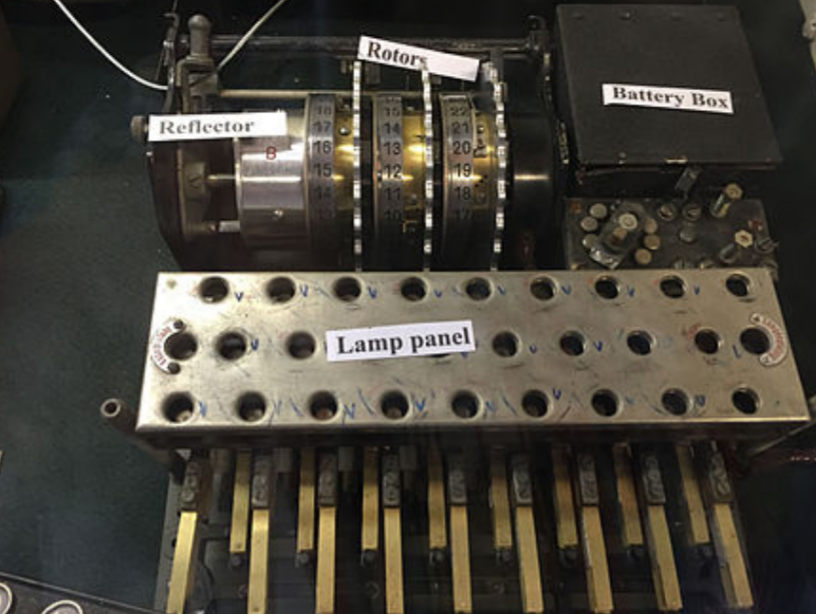
\includegraphics[scale=.4]{images/15.PNG}
	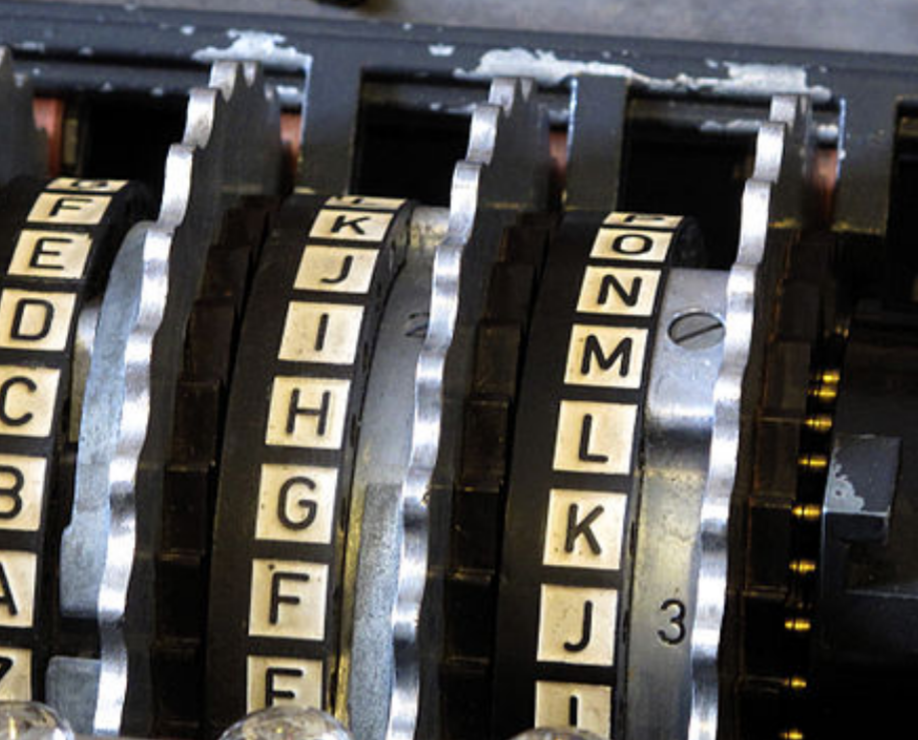
\includegraphics[scale=.33]{images/16.PNG}
\end{center}
Il riflettore è anch'esso un rotore modificato. Per aumentare lo spazio delle chiavi si aggiunge una \emph{plugboard} cioè una batteria di connettori che mette in corrispondenza diretta due lettere (in un certo senso è come se scambiassi di posizione due lettere, premo una e in realtà ne sto premendo un'altra). 
\begin{center}
	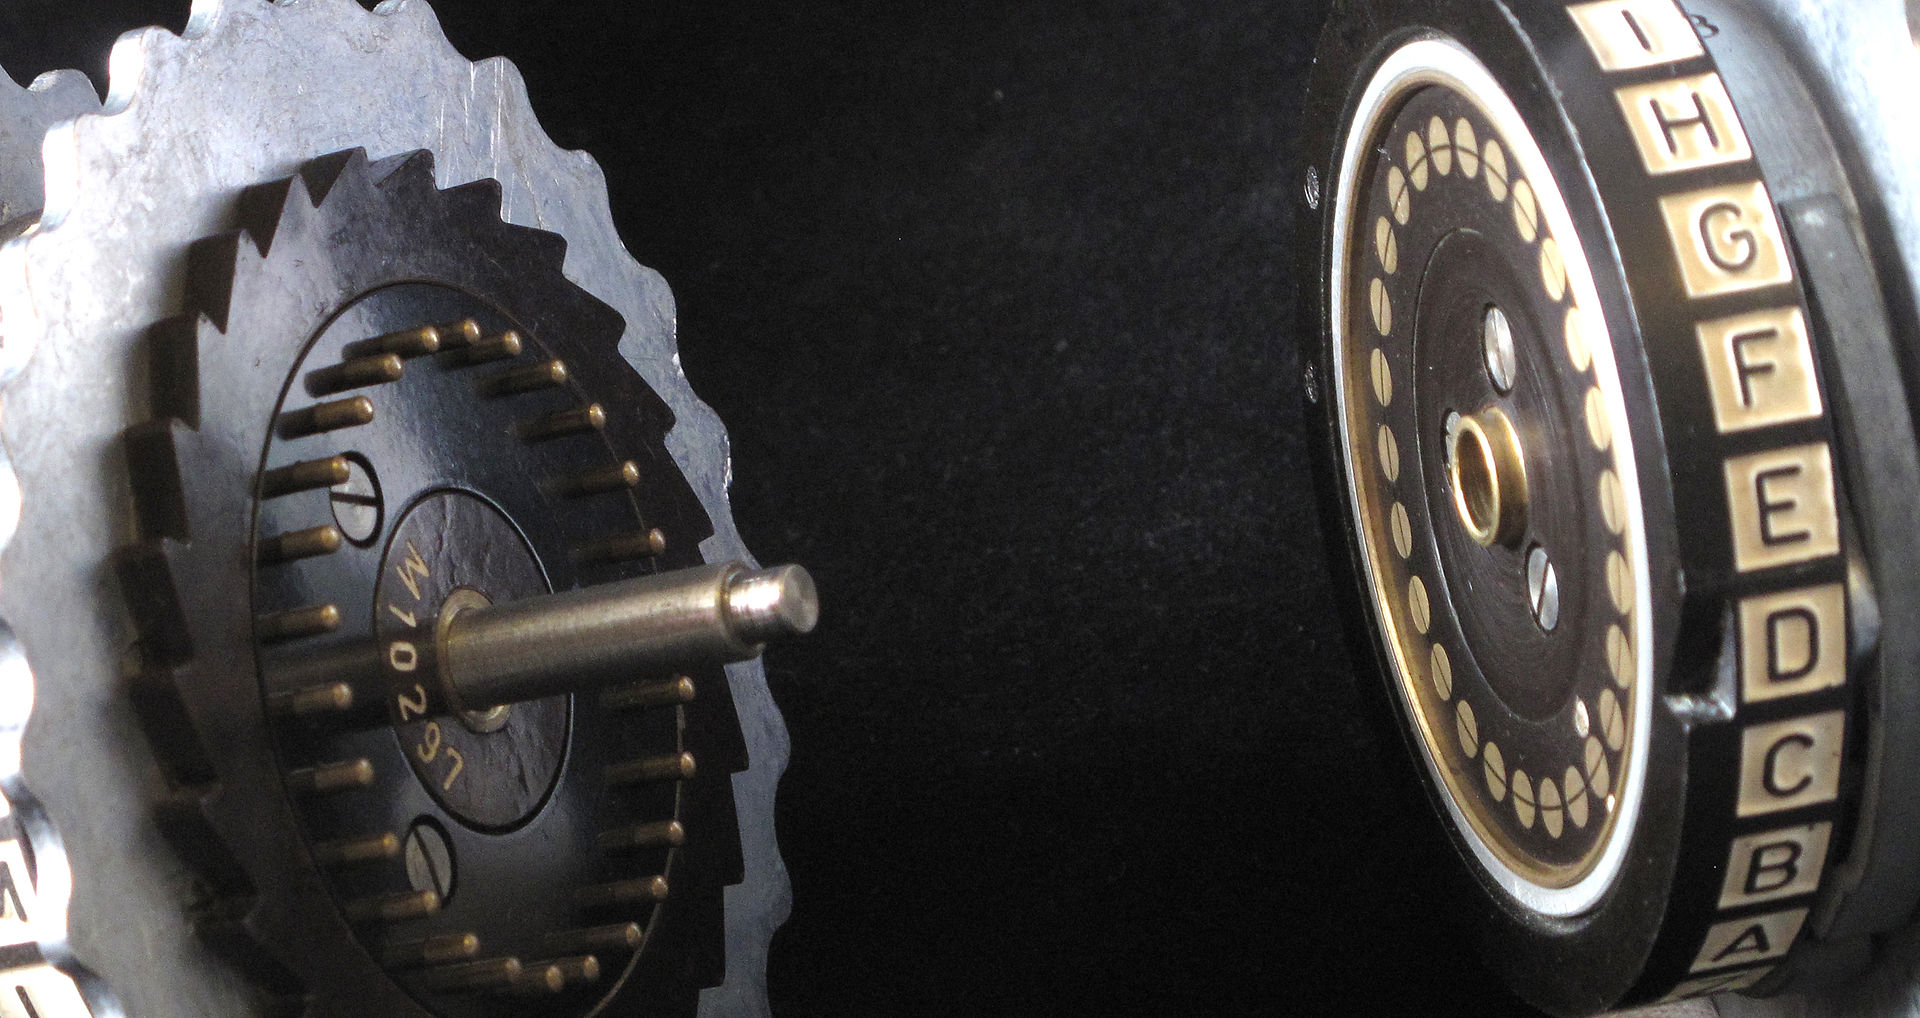
\includegraphics[scale=.35]{images/17.jpg}
\end{center}
Ogni rotore rappresenta la permutazione di un alfabeto. Possiede due facce : \emph{pad} e \emph{pin}, ciascuna con ventisei contatti elettrici disposti in cerchio e ciascuno associato a una particolare lettera. Si ha un cablaggio fisso che collega i contatti di una faccia con quelli di un'altra.
\begin{center}
  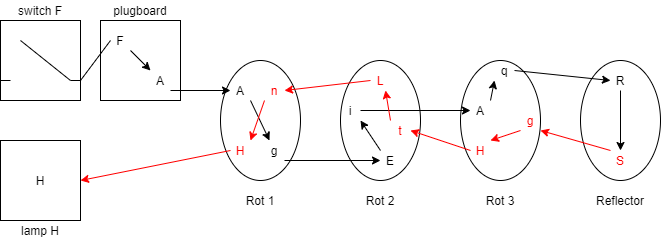
\includegraphics[width = 350pt]{images/Enigma.png}
\end{center}

\begin{itemize}
	\item Per costruzione una lettera non è mai cifrata con se stessa. Questa proprietà e quella di riflessione sono state utilissime nel rompere questo sistema.
	\item I rotori non sono fissi.
	\begin{itemize}
		\item Il primo rotore avanza di un passo per ogni lettera battuta sulla tastiera.
		\item Dopo 26 passi il primo rotore torna sulla posizione iniziale, quindi si muove di una posizione il secondo rotore.
		\item Dopo la rotazione completa del secondo rotore si muove di un passo il terzo rotore.
	\end{itemize}
	Questa cosa comporta una chiave cambiata ad ogni passo.
	\item Le permutazioni sono 26 per il primo rotore rispetto al secondo, 26 del secondo rispetto al terzo, 26 del terzo rispetto al riflettore: $$26 \cdot 26 \cdot 26 = 17.576$$ chiavi se i rotori sono immutabili e noti a chiunque ne avesse una copia. 
	\item Si aumentano le chiavi scambiando l'ordine dei rotori, quindi si sale a ${26}^3 \cdot \left(3!\right) > 10^5$.
	\item Aggiungendo le plugboard si possono scambiare 6 coppie di caratteri per ogni trasmissione, si arriva quindi ad una sequenza di 12 caratteri per descrivere il cablaggio: le combinazioni possibili sono $$\binom{26}{12} \approx 10^7$$ Scelte le lettere va scelta la loro ordinazione: 
	$$\binom{26}{12} \cdot 12!$$
	In realtà dobbiamo escludere delle permutazioni, quelle che lasciano lo stesso effetto, quindi dividiamo per $6!$ e per $2^6$
	\begin{center}
		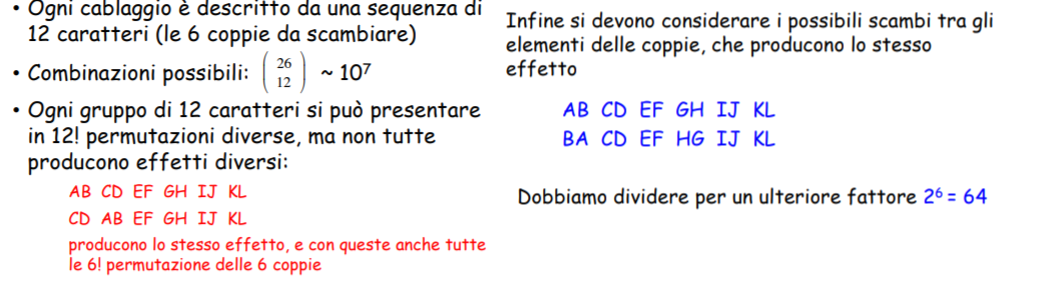
\includegraphics[scale=.75]{images/26.PNG}
	\end{center}
\end{itemize}

	\part{Cifrari perfetti}
\chapter{Introduzione}
I cifrari perfetti sono cifrari che offrono una \underline{\textbf{sicurezza incondizionata}}, proteggono le informazioni con certezza assoluta di fronte a qualsiasi potenza di calcolo. Solo chi è in possesso della chiave può decifrare. Un attacco a forza bruta non può rompere la cifratura (pur avendo risorse computazionali spropositate).

\paragraph{Costo e crittografia di massa} Si paga un caro prezzo nella loro implementazione, infatti questi cifrari sono usati solo in pochi ambiti,
per la crittografia di massa si preferisce avere una sicurezza computazionale scommettendo su $P \neq NP$.

\paragraph{Definizione informale} Questo concetto è stato formalizzato da Shannon (nel 1949, in realtà prima) informalmente un cifrario è perfetto se la sicurezza è garantita qualunque sia l'informazione carpita dal canale.
\section{Formalizzazione del concetto di \emph{cifrario perfetto}}
Abbiamo lo spazio dei messaggi $MSG$ e lo spazio dei crittogrammi $CRITTO$. Abbiamo poi le variabili aleatorie $M \in MSG$, che descrive il comportamento del mittente, e $C \in CRITTO$, che descrive il processo di comunicazione sul canale. \begin{itemize}
	\item Ricorriamo alla teoria della probabilità per definire:
	\begin{itemize}
		\item $P(M=m)$ : probabilità che il mittente voglia spedire il messaggio $m$ al destinatario
		\item$ P(M=m | C=c)$ : probabilità condizionata (a posteriori) che il messaggio inviato sia effettivamente $m$, dato che sul canale transita il crittogramma $c$
	\end{itemize}
\item Si suppone che il crittoanalista conosca tutto il sistema tranne la chiave. Conosce:
\begin{itemize}
	\item distribuzione di probabilità con cui il mittente invia un messaggio
	\item conosce il cifrario
	\item conosce lo spazio delle chiavi K
\end{itemize}
\end{itemize}
\paragraph{Definizione} {Un cifrario è perfetto se} $\forall m \in MSG$, $\forall c \in CRITTO$ vale:
$$ P(M=m  \mid  C=c) = P(M=m) $$
Cioè: la conoscenza di C non ci permette di dire nulla sul messaggio.

\subsection{Esempi di cifrari non perfetti (casi estremi)}
Supponiamo che ci sia un messaggio $\overline{m}$ che il mittente invia con probabilità $0<p<1$.
$$P(M=\overline{m}) = p$$
Cosa succede in assenza dell'uguaglianza alla base della definizione di cifrario?
\paragraph{Esempio estremo 1}  Supponiamo di avere probabilità uguale ad $1$.
$$\exists \overline{m}, \overline{c} : P(M=\bar{m} \mid C=\bar{c}) = 1$$
Il caso è estremo. Con probabilità $1$ sicuramente il messaggio associato al crittogramma $\overline{c}$ è $\overline{m}$, dunque aumenta la nostra conoscenza sul sistema. 

\paragraph{Esempio estremo 2} Supponiamo una situazione dove la probabilità è nulla
$$\exists \overline{c} : P(M=\overline{m} | C=\overline{c}) = 0$$
ci permette di dire che se passa $\overline{c}$ non è stato sicuramente spedito il messaggio $m$. Anche qui la nostra conoscenza aumenta: il sistema non è perfetto!

\paragraph{Quindi} In un cifrario perfetto la conoscenza complessiva del crittoanalista non cambia dopo che è stato osservato un crittogramma in transito:
\[\boxed{\text{$m$ e $c$ sono del tutto scorrelati, c appare essere una sequenza casuale}}\]

\section{Teorema di Shannon}
\emph{In un cifrario perfetto il numero delle chiavi deve essere maggiore o uguale al numero dei messaggi possibili}
\paragraph{Dimostrazione}Vogliamo dimostrare che $N_k \geq N_m$
\begin{align*} 
	N_m &= \#\{m \in MSG : P(M=m)>0\}\,\,\,\,\,\,\text{Num. dei messaggi possibili}\\
	N_k &= \#\{\text{insieme delle chiavi}\}
\end{align*}
Supponiamo per assurdo che $N_k < N_m$, e prendiamo un crittogramma $c$ tale $$P(C=c)>0$$Cerchiamo di contare quanti messaggi corrispondono a questo crittogramma.
\begin{itemize}
	\item Supponiamo che corrispondano $S$ messaggi. Essi sono i messaggi che posso ottenere decifrando $c$ con tutte le chiavi possibili. Decifro con la chiave $k1$ e ottengo $m1$, decifro con la chiave $k2$ e trovo $m2$, decifro con la chiave $k3$ e ottengo sempre $m2$ (non lo posso escludere), e così via...
	\begin{center}
		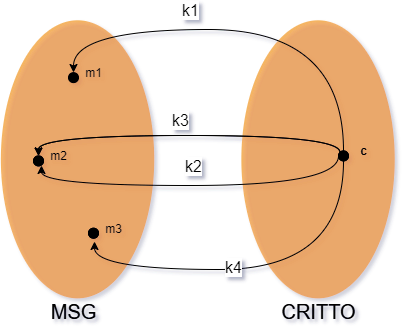
\includegraphics[width = 250pt]{images/Shannon_proof.png}
	\end{center}
	\item Si ha necessariamente $S \leq N_k$ (posso ottenere al più $N_k$ messaggi, non di più).
	\item Poichè abbiamo iniziato con l'ipotesi $N_k < N_m$ otteniamo
	$$S \leq N_k < N_m$$
	quindi
	$$S < N_m$$
	Il numero di messaggi associati al crittogramma $c$ ($S$) è strettamente minore del numero di messaggi possibili.
	\item Appurato che  $S < N_m$ affermiamo che deve esistere un messaggio $m$ con probabilità $P(M=m)>0$ tale che
	$$ P(M=m \mid C=c) = 0 $$
	decifrando $c$ esisterà un $m$ che sicuramente non è il messaggio.
	\item \textbf{Inferisco della conoscenza, quindi contraddico il cifrario perfetto}. Ne deriva quindi che $N_k \geq N_m$. Per usare un cifrario perfetto mi serve quindi una chiave lunghissima!
\end{itemize} 
$\hfill\blacksquare$

\chapter{\emph{One-Time Pad}}
\begin{framed}
	\noindent \textbf{Domanda da esame}. Qual è lo svantaggio principale del cifrario One-Time Pad?
\end{framed} 
\section{Cifratura e decifratura}
Il \emph{One-Time Pad} è un cifrario precedente Shannon, simile ad un Vigenère con chiave lunga quanto il messaggio ma su un alfabeto binario. Nasce nel 1917 da Mauborge e Vernam. \emph{Pad} significa \emph{blocco}, \emph{One-Time} poichè la chiave può essere utilizzata una sola volta.

\paragraph{Ragionamento} Come alfabeto si usa \{0, 1\}. MSG, CRITTO, KEY sono spazi delle sequenze binarie e l'algoritmo di cifratura è noto a tutti ed è lo XOR (somma modulo 2). Supponiamo quindi $m, k \in \{0, 1\}^{n}, n > 0$:
\begin{align*}
	c &= C(m, k) = m \oplus k\\
	 m &= D(c, k) = c \oplus k
\end{align*}

\paragraph{Esempio} Dato $n=5, m=10110, k=01011$ otteniamo
$$c=11101$$
Se io riapplico nuovamente lo XOR ottengo di nuovo
$$m=10110$$
Questo ci torna poichè
$$m = c \oplus k = m \oplus k \oplus k = m \oplus 0 = m$$
\paragraph{Necessità di cambiare la chiave} La chiave deve essere cambiata frequentemente. Supponiamo di non  farlo
\begin{align*}
	c_1 = m_1 \oplus k
	&&
	c_2 = m_2 \oplus k
\end{align*}
Proviamo a fare il seguente calcolo
$$ c_1 \oplus c_2 = m_1 \oplus k \oplus m_2 \oplus k = m_1 \oplus m_2 $$
non ottengo la chiave, ma so che l'operatore XOR restituisce lo zero se due caratteri sono uguali. Il crittoanalista ha imparato qualcosa di nuovo. 
\paragraph{Sicurezza} L'unica informazione ottenibile dal one-time-pad è \textbf{la lunghezza del messaggio}. La sicurezza del One-Time Pad non è computazionale: l'attacco forza bruta non ha alcun senso perchè da tutte le chiavi possibili otteniamo un vasto insieme di messaggi possibili. Mittente e destinatario, a volte, si mandano messaggi privi di senso per rafforzare la sicurezza.





\section{Teorema su \emph{One-time pad} perfetto e minimale}
\emph{One-Time Pad} è un cifrario perfetto e minimale (usa un numero minimo di chiavi) se:
\begin{itemize}
    \item tutti i messaggi hanno lunghezza $n$, se più corti li paddo, se più lunghi li divido in blocchi;
    \item tutte le sequenze di $n$ bit hanno probabilità maggiore di zero di essere inviate (tutte le sequenze di bit sono messaggi, ogni tanto mittente e destinatario si scambiano sequenze prive di significato);
    \item si usano chiavi scelte perfettamente a caso per ogni messaggio.
\end{itemize}
Chiaramente la cosa è complessa: la chiave deve essere lunga quanto il messaggio e deve essere cambiata ogni volta.
\begin{framed}
\noindent Si ricordi la definizione di probabilità condizionata:
$$ P(M=m \mid C=c) \triangleq \frac{P(M=m\text{ e }C=c)}{P(C=c)} $$
Al numeratore abbiamo la probabilità che entrambi gli eventi siano avvenuti: che Alice invii il messaggio $m$ e che l'abbia cifrato ottenendo il crittogramma $c$. Si divide per la probabilità che stia transitando $c$ sul canale di comunicazione.
\end{framed} 
\begin{framed}
	\noindent \textbf{Domanda da esame}. Spiegare con precisione matematica e proprietà di linguaggio perché il cifrario One-Time Pad su messaggi di $n$ bit non può essere ritenuto perfetto se la chiave non è scelta perfettamente a caso
\end{framed}
\paragraph{Dimostrazione perfettezza}
\begin{itemize}
	\item \textbf{Tesi}. La tesi è la definizione di cifrario perfetto:
	$$ \forall m \in MSG, \forall c \in CRITTO $$
	$$ P(M=m \mid C=c) = P(M=m) $$
	\item Stimiamo il numeratore. Dato un messaggio $m$ vogliamo ottenere un crittogramma $c$: per le proprietà dello XOR esiste una sola chiave $k$ in grado di farmi ottenere $c$ a partire da $m$
	$$ \exists! \, k \in \text{KEY}: m \oplus k = c $$
	Segue che la probabilità di ottenere il crittogramma $c$ dal messaggio $m$ è pari alla probabilità di scegliere casualmente la chiave $k$: $\frac{1}{2^n}$ (formulina già trovata, quando abbiamo introdotto la casualità)

	$$\forall c \in \text{CRITTO}\,\,P(C=c)=\frac{1}{2^n}$$
	Nella formula non abbiamo alcuna dipendenza della probabilità dal messaggio (si pensi all'ipotesi 3 del teorema), quindi possiamo scrivere la probabilità nel seguente modo
	$$ P(C=c\text{ e }M=m) = P(M=m) \cdot P(C=c) $$
	\item Prendiamo la definizione di probabilità condizionata e sostituiamo
	$$
	P(M=m \mid C=c) = \frac{P(M=m\text{ e }C=c)}{P(C=c)} = \frac{P(M=m) \cdot \cancel{P(C=c)}}{\cancel{P(C=c)}}
	$$
	siamo arrivati alla definizione di cifrario perfetto!
\end{itemize}
$\hfill\blacksquare$






\paragraph{Dimostrazione minimale}
Sappiamo da Shannon che il numero delle chiavi deve essere maggiore o uguale rispetto al numero dei messaggi $$N_k \geq N_m$$ ma nel one-time pad su lunghezza $n$ ho $2^n$ messaggi possibili, e $2^n$ crittogrammi possibili
$$N_k = N_m= N_{CRITTO} = 2^n$$
Anche le chiavi sono sequenze di bit e ne uso il numero minore possibile. Ricordiamo che tutte le sequenze di $n$ bit sono messaggi possibili: l'attacco forza bruta non ha senso.

$\hfill\blacksquare$


\section{Riduzione della dimensione della chiave}
Cerchiamo di ridurre la dimensione delle chiavi. Pensiamo alla lingua inglese, dove i messaggi significativi sono solo $\alpha^{n}$ con $\alpha = 1.1$
$$\alpha^n << 2^n$$
Poniamo $N_m = \alpha^n$ dato che $N_k = 2^t \geq N_m = \alpha^n$. Vogliamo individuare il numero di bit $t$, necessari affinchè 
\begin{align*}
	2^t \geq \alpha^n \longrightarrow t \cdot \log_2 2 \geq \log_2\alpha^n &= n \cdot \log_2\alpha \\ t \geq \log_2\alpha^n &= n \cdot \log_2\alpha \longrightarrow t \geq 0.12 \cdot n
\end{align*}
Posso quindi usare chiavi molto più corte: $\approx 10\%$ di $n$.

\paragraph{Come fare?} Genero i $t$ bit randomicamente e li estendo in maniera deterministica su $n$ bit (funzione che dato in ingresso una sequenza su $t$ bit mi restituisce una sequenza su $n$ bit, sempre lo stesso output con lo stesso input).
Dobbiamo però metterci al riparo dall'attacco forza bruta: è fondamentale che coppie diverse di
$(m, k)$ producano lo stesso crittogramma. Per far ciò il $\#(m, k)$ deve essere di molto maggiore di $\#CRITTO$:
$$ \alpha^n \cdot 2^t >> 2^n \xrightarrow{} t >> 0.88n$$
In definitiva ci serve $t >> 88\%n$ quindi non si ha una grande compressione della chiave.

	\part{Cifrari simmetrici moderni}
\chapter{\emph{Data Encryption Standard} (DES)}
\section{Introduzione e principi di Shannon}
Il \emph{Data Encryption Standard} è un cifrario simmetrico che è stato lo standard per la crittografia di massa fino all'avvento dell'AES Pur non essendo più usato è importante conoscerlo: i cifrari moderni si basano sulla struttura del DES. Il DES è il primo algoritmo a basarsi sui principi di Shannon.
\begin{itemize}
    \item \textbf{Diffusione}: ogni singolo carattere del crittogramma dipende da \underline{\textbf{tutti}} i caratteri del testo in chiaro.
    \item \textbf{Confusione}: combinare testo in chiaro e chiave in modo complesso in modo che osservare il crittogramma non possa portare a separare le due sequenze (testo in chiaro e chiave).
\end{itemize}
Questi principi sono importanti per la resistenza agli attacchi di crittoanalisi statistica.

\section{Storia}
Nasce nel 1972 quando NBS (\textit{National Bureau of Standard}) ora NIST (\textit{National Institute for Security and Technology}) chiese la creazione di un algoritmo di crittografia simmetrica standard (standard poichè ogni compagnia usava un proprio sistema crittografico). 
\paragraph{Richieste dell'ente} In particolare le richieste erano:
\begin{itemize}
    \item sicurezza basata sulla segretezza della chiave e non sul processo di cifratura e decifrazione (tutto pubblico tranne la chiave);
    \item l'algoritmo doveva essere efficiente sia in software che in hardware;
    \item la sua sicurezza doveva essere certificata da terzi (un terzo che garantiva la sicurezza del sistema, con sistemi proprietari rimane il dubbio sull'affidabilità).
\end{itemize}
Il primo bando andò deserto, al secondo l'IBM propose \emph{Lucifer} e lo lasciò studiare alla NSA che introdusse alcune variazioni:
\begin{itemize}
    \item riduzione della dimensionee della chiave da 128 bit a 56 bit;
    \item modifiche nella la S-box (che vedremo a breve, componente cruciale del cifrario).
\end{itemize}
La IBM sospettò che la NSA volesse rende più facile la rottura del cifrario, ma alla fine accettò le modifiche dopo averle studiate a fondo. 
\paragraph{Pubblicazione e rinnovo periodico} Il cifrario è stato reso pubblico nel 1977 con licenza d'uso gratuito. La certificazione era rinnovata periodcamente valutando le evoluzioni nella crittoanalisi. Quando si trova un attacco con costo inferiore a quello di un attacco forza bruta (sullo spazio delle chiavi) allora il cifrario si dice forzato.
\paragraph{3-DES (triplo DES)} E' rimasto in vita fino al 1999 quando ne è stato sconsigliato l'uso per una versione più aggiornata: il 3-DES.
\paragraph{AES} Nel 2005 anche il 3-DES diventa sconsigliato a fronte dell'AES proposto nel 2000 ed entrato nel 2001 all'utilizzo di massa. Ad oggi l'AES non è stato ancora rotto.

\section{Cifratura}
Nel DES la cifratura avviene per blocchi di 64 bit, la chiave è di 64 bit in cui 56 sono casuali ed 8 sono di parità (ogni 7 un bit di parità, serve per verificare che la chiave venga acquisita in modo corretto).
La cifratura si compone di $r=16$ fasi in cui si ripetono le stesse operazioni.
\begin{center}
	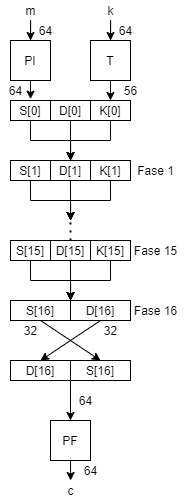
\includegraphics[width = 100pt]{images/DES_1.png}
\end{center} 
Nel grafico individuiamo:
\begin{itemize}
	\item m: blocco del messaggio (abbiamo in ingresso il blocco a 64 bit da criptare)
	\item k: chiave segreta con i bit di parità (64 bit, di cui 8 bit di parità)
	\item PI e PF: permutazione iniziale e finale (non ci sono sempre)
	\item c: corrispondente blocco del crittogramma (risultato finale dopo la $16-$esima fase)
\end{itemize}
Abbiamo in ingresso il messaggio $m$ a 64 bit e la chiave a 64 bit (di cui otto di parità). Permutiamo i bit del messaggio con $PI$, permutiamo anche i bit della chiave con $T$ ottenendo $K[0]$ Attenzione: $T$ restituisce solo 56 bit perchè scarta i bit di parità (di cui si conosce la posizione). A questo punto dividiamo il messaggio $m$ permutato (eventualmente permutato) in due blocchi: $S[0]$, $D[0]$. Eseguiamo una serie di fasi e alla fine, dopo l'ultima, scambiamo di posizione i blocchi $S[16]$ e $D[16]$. Eventualmente permutiamo.



\paragraph{Funzioni} In ogni fase $i=1,2,\dots,16$ andiamo ad applicare le seguenti funzioni:
\begin{align*}
	\text{S}[i] &= \text{D}[i-1]\\
	\text{D}[i] &= \text{S}[i-1] \oplus f\left(\text{D}[i-1],\text{K}[i-1]\right)
\end{align*}
Si scambiano le due metà dell'input, e D viene ottenuto con l'operatore XOR bit a bit tra $\text{S}[i-1]$ e una funzione non lineare $f\left(\text{D}[i-1],\text{K}[i-1]\right)$ (la S-box detta prima). Con le permutazioni e gli scambio realizzo la \textbf{diffusione} (lo vediamo perchè alterando un solo bit del messaggio in chiaro si ha un drastico cambiamento nell'intero crittogramma), con la S-box la \textbf{confusione} (la S-box prende in ingresso la chiave).

\paragraph{PI, PF e T} PI, PF e T sono delle tabella che vanno lette per riga:
\begin{center}
	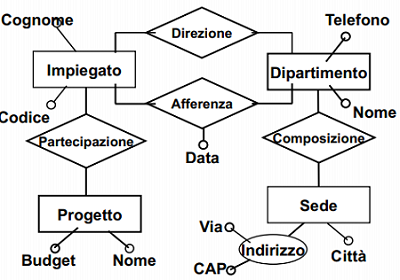
\includegraphics[scale=.5]{images/17.PNG}
\end{center}

\paragraph{Fase} La fase $i$-esima del DES è rappresentata dal seguente schema.
\begin{figure}[H]
    \centering
    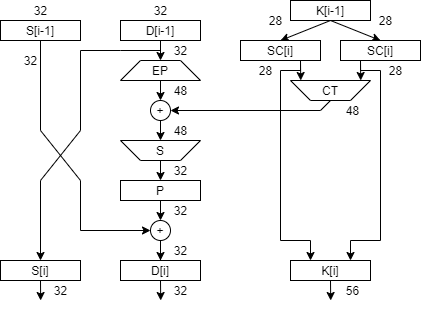
\includegraphics[width = 280pt]{images/DES_2.png}
\end{figure}
\noindent Abbiamo come input i blocchi $S[i-1]$, $D[i-1]$ (ottenuti dalla fase precedente, o i blocchi iniziali posti come indicato prima) e $K[i-1]$ (la chiave, alterata ad ogni step). La chiave viene divisa in due metà da 28 bit ciascuno. Su ciascuna metà si esegue uno shift ciclico (SC) a sinistra, dove il numero di posizioni dipende dall'indice della fase:
\begin{itemize}
	\item 1 se $i \in \{1, 2, 9, 16\}$
	\item 2 altrimenti
\end{itemize}
A questo punto i blocchi ottenuti vengono usati in due modi:
\begin{itemize}
	\item concatenati e posti come $K[i]$ (chiave usata nel prossimo step)
	\item concatenati e posti in ingresso in $CT$.
\end{itemize}
Il blocco CT permuta e scarta alcuni bit (si passa da 56 a 48 bit).Per quanto riguarda le due sequenze da 32 bit ($S[i-1]$ e $D[i-1]$):
\begin{itemize}
	\item pongo in $S[i]$ il contenuto di $D[i-1]$
	$$\text{S}[i]=\text{D}[i-1]$$
	\item pongo i bit di $D[i-1]$ in ingresso ne blocco EP, che permuta i bit e li espande (duplicazione di alcuni bit, si passa da 32 bit a 48 bit);
	\item applico lo XOR alle due sequenze a 48 bit (quella ottenuta da EP e quella ottenuta da CT)
	\item applico la S-box (che garantisce la non linearità della funzione, si passa da 48 a 32 bit);
	\item permuto i 32 bit ottenuti dalla S-box e applico l'operatore XOR tra questi ed $S[i-1]$.
\end{itemize}

\paragraph{Funzioni CT ed EP}
\begin{center}
	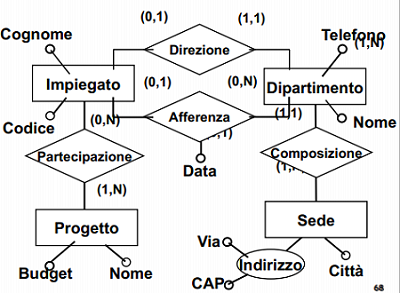
\includegraphics[scale=.5]{images/18.PNG}
\end{center}

\paragraph{S-Box} La S-box implementa 8 funzioni booleane a 6 input e a 4 output (in bit).
\begin{center}
    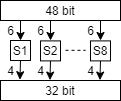
\includegraphics[width = 100pt]{images/DES_3.png}
\end{center}
Queste funzioni sono rappresentate attraverso delle tavola di verità, che vanno però lette in maniera particolare (di seguito la tabella di S1). Prendiamo il seguente esempio...
\begin{table}[ht!]
    \centering
    \small
    \begin{tabular}{c|c c c c c c c c c c c c c c c c}
        & 0 & 1 & 2 & 3 & 4 & 5 & 6 & 7 & 8 & 9 & 10 & 11 & 12 & 13 & 14 & 15 \\
        \hline
        0 & 14 & 4 & 13 & 1 & 2 & 15 & 11 & 8 & 3 & 10 & 6 & 12 & 5 & 9 & 0 & 7 \\
        1 & 0 & 15 & 7 & 4 & 14 & 2 & 13 & 1 & 10 & 6 & 12 & 11 & 9 & 5 & 3 & 8 \\
        2 & 4 & 1 & 14 & 8 & 13 & 6 & 2 & 11 & 15 & 12 & 9 & 7 & 3 & 10 & 5 & 0 \\
        3 & 15 & 12 & 8 & 2 & 4 & 9 & 1 & 7 & 5 & 11 & 3 & 14 & 10 & 0 & 6 & 13 \\
    \end{tabular}
\end{table}

\noindent Supponiamo di avere 010011: prendo gli estremi 0 ed 1 ed uso questo come indice per la riga, prendo poi i 4 bit centrali (1001) e lo uso come indice di colonna. Accedo quindi a (1, 9) $\xrightarrow{} 06$.

\paragraph{Perché è importante che non sia lineare?} Perché $$f(x \oplus y) \neq f(x) \oplus f(y)$$ ed è cruciale ai fini del funzionamento!

\section{Proprietà del DES con $m,c$ complementati}
Consideriamo i crittogrammi $c$, $c^{*}$, con il messaggio $m$ e la chiave $k$:
\begin{align*}
	c &= C_{DES}(m, k)&	c^{*} &= C_{DES}(\overline{m}, \overline{k})
\end{align*}
Abbiamo visto che prima della S-box applichiamo l'operatore XOR (ricordarsi $x \oplus 1=\overline{x}$)
$$ \bar{m_i} \oplus \bar{K_i} = (1 \oplus m_i) \oplus (1 \oplus K_i) = m_i \oplus K_i $$
Date le coppie $<m,k>, <\overline{m},\overline{k}>$ l'input della S-box \textbf{\underline{è lo stesso}}, dunque dalla S-box esce lo stesso output. In realtà il crittogramma restituito è il complemento
$$c^{*}=\overline{c}$$
Questo perchè nello XOR finale si ha complementazione in uno solo dei due blocchi (abbiamo un blocco posto direttamente che può essere complementato o no e un altro da cui otteniamo la stessa sequenza - \textit{S-box} - indipendentemente dall'essere complementato o no).
\paragraph{Esempio}
\begin{center}
	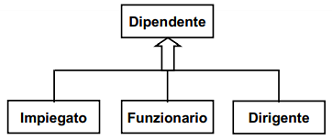
\includegraphics[scale=.75]{images/21.PNG}
\end{center}
\[\boxed{\text{\url{https://fauzanakmalh1.github.io/Simplified-DES-Calculator/}}}\]

\section{Attacchi al DES}
Gli attacchi al DES sono tutti attacchi a forza bruta:
\begin{itemize}
    \item \textbf{architetture appositamente progettate per attaccare il DES} e quindi velocizzare criptazione e decriptazione (con 1M\$ si costruiva una macchina che forzava il DES in 35 minuti);
    \item \textbf{distribuire lo spazio delle chiavi tra più utenti}, è più economico e la velocità dipende da quanti utenti vengono coinvolto.
\end{itemize}
\paragraph{\emph{challenges} di RSA} Nel 1997 la compagnia RSA ha offerto una ricompensa di diecimila dollari a chi avrebbe decifrato un crittogramma (non tanto trovare il messaggio, ma la chiave che ha prodotto quel particolare crittogramma attraverso il DES): in 5 mesi esplorando il 25\% delle chiavi viene risolta la sfida e trovata la chiave. Nel 1998 è stata lanciata una seconda sfida: ci vollero 39 di giorni esplorando 85\% delle chiavi.
\begin{align*}
	1997:\,\,&\text{strong cryptography makes the world a safer place}\\1998:\,\,&\text{many hands make light work}
\end{align*}

\subsection{Attacchi esaurienti} Le chiavi possibili sono $2^{56}$, 64 di queste chiavi sono rimosse perché con regolarità. Ricordando che:
\begin{align*}\boxed{C(m, k) = c}&&\boxed{\bar{c} = C(\bar{m}, \bar{k})}\end{align*}
si possono dimezzare le chiavi passando da $2^{56}$ a $2^{55}$ ($2^{56}=2\cdot 2^{55}$, 55 bit di sicurezza). Questo è un tipo di \textbf{attacco chosen plain-text} (scelto perchè i messaggi in chiaro devono avere una certa relazione) in cui il crittoanalista si procura delle coppie $$<m, c_1>, <\bar{m}, c_2>$$ Si inizia ad esplorare le chiavi e per ognuna si controlla:
\begin{itemize}
    \item $C(m, k) = c_1$: k probabilmente è la chiave
    \item $C(m, k) = \bar{c_2}$: $\bar{k}$ probabilmente è la chiave
    \item Se $c_1 \neq \bar{c_2}$ si prova un'altra chiave (k e $\bar{k}$ non lo sono)    
\end{itemize}
Possiamo dire
$$C(m,k) = \bar{c_2} \iff C(\bar{m},\bar{k}) = \bar{\bar{c_2}} = c_2$$
Escludo quindi due chiavi alla volta ($C(m,k)$ si calcola una volta soltanto, mentre la complementazione è operazione "tranquilla").

\subsection{Crittoanalisi differenziale} Nel 1990 sono stati scoperti attacchi di \emph{crittoanalisi differenziale} (da Bihan e Shamir).
\begin{itemize}
	\item E' un attacco di tipo \textbf{chosen plain-text} in cui il crittoanalista si procura $2^{47}$ coppie $<m,c>$ (messaggio scelto dal crittoanalista, obv).
	\item I messaggi sono scelti in modo tale da avere differenze particolari, il crittoanalista va a verificare le variazioni nel crittogramma. Si sfruttano le similitudini per arrivare alla chiave.
	\item Si assegnano delle probabilità alle singole chiavi, ed emerge poi quella più probabile.
\end{itemize}
\paragraph{Costo} Dato che le fasi sono 16 si ha un costo di questo attacco pari a $2^{55.1}$, poco più di una ricerca esaustiva (quindi nulla di interessante sul piano pratico). Con un numero di fasi minori, per esempio $8$, il costo si riduce drasticamente e allora il costo è minore rispetto alla ricerca esaustiva.

\subsection{Crittoanalisi lineare} Nel 1993 sono stati scoperti attacchi di \emph{crittoanalisi lineare} che consistono nella costruzione di una \underline{approssimazione lineare} della S-box che permette di inferire taluni bit della chiave, il resto si \textit{bruta}.
\paragraph{Costo} Si scende a $2^{43}$ coppie $<m, c>$ ed è di tipo known plain-text. Metodo più efficiente del forza bruta.

\section{Varianti del DES}
Il DES è sensibile agli attacchi di crittoanalisi differenziale e lineare, per renderlo più robusto si sono introdotte delle varianti. 
\subsection{Scelta indipendente delle sottochiavi}
Anziché generare le sottochiavi di fase a partire dalla chiave principale si scelgono manualmente.
E' come passare da 56 bit a $16 \cdot 48 = 768$ bit di chiave. \paragraph{Problema risolto?} Non abbiamo un effettivo aumento della sicurezza perché è sempre vulnerabile ad attacchi differenziali: si passa da 768 bit di sicurezza a 61 bit ($2^{61}$ la complessità).

\subsection{Cifratura multipla: 2DES}
Questa variante ha avuto maggiore successo rispetto alla precedente. L'idea è di applicare due volte la cifratura, di comporre il DES con se stesso:
$$ \forall k_1, k_2, k_3: C_D(C_D(m, k_1), k_2) \neq C_D(m, k_3) $$
applicare due volte la cifratura DES non è uguale ad applicarlo una sola volta.
Si arriva ad uno spazio delle chiavi di $2^{112}$.
\paragraph{Problema risolto?} L'attacco \emph{meet-in-the-middle} fa scendere la sicurezza a 57 bit di sicurezza:
$$ c = C(C(m,k_1), k_2) $$
facciamo la decifrazione di $C$ con la chiave $k_2$ (tolgo la cifratura più esterna)
$$ D(c,k_2) = C(m,k_1) $$
possiamo quindi prendere una coppia $<m, c>$:
\begin{itemize}
	\item $ \forall k_1 \text{ calcolo e salvo } C(m, k_1) \xrightarrow{} 2^{56} \text{ cifrature (tutte)}$
	\item $ \forall k_2 \text{ calcolo e verifico corrispondenza di } D(c, k_2) \xrightarrow{} 2^{56} \text{ cifrature (al più) }$
\end{itemize}
Cercando nella lista delle cifrature, so che esisterà una coppia $<k_1, k_2>$ per la quale c'è la corrispondenza:
$$ D(c, \bar{k_2}) = C(m, \bar{k_1}) $$
Questo attacco costa quindi $2^{56} + 2^{56} = 2 \cdot 2^{56} = 2^{57}$ al più, tra cifrature e decifrature. Cioè l'aumento di complessità dovuto alla doppia cifratura non è di $N^2$ ma di $2N$
$$2N << N^2$$


\subsection{Cifratura multipla: 3DES}
Nella pratica non si è fatta una doppia cifratura. 
\begin{itemize}
    \item \textbf{2TDEA} (proposta a due chiavi):
        $$ c = C\left(D(C(m, k_1), k_2), k_1\right) $$
        $k_1$ e $k_2$ sono chiavi di 56 bit tra di loro indipendenti. Si sceglie questa modalità (CDC invece di CCC) per mantenere la compatibilità abilitati a usare un singolo DES. Se pongo $k_1 = k_2$ ottengo il DES normale (cifratura singola).
        
        {Attenzione}: CDC non è più robusto di CCC. Un attacco \emph{meet-in-the-middle} ha un costo di 112 bit.
    \item \textbf{3TDEA} (\textit{triple data encryption algorithm}):
        $$ c = C(D(C(m, k_1), k_2), k_3) $$
        $k_1$, $k_2$, $k_3$ sono chiavi a 56 bit. Si hanno chiavi di $3 \cdot 56 = 168$ bit. In realtà è vulnerabile ad attacchi \textit{meet-in-the-middle} quindi la sicurezza scende da 168 bit a 112 bit di sicurezza.
        
        Per ottenere il messaggio decifriamo usando le chiavi in ordine inverso
        $$m=D\left(C(D(c,k_3),k_2),k_1\right)$$
        Osserviamo banalmente che
        $$C(m,k_1)=C(D(c,k_3),k_2)$$
        come prima 
        $$\forall k_1 \text{ calcolo e salvo } C(m,k_1)$$
        successivamente
        $$\forall k_2,k_3 \text{ calcolo } C(D(c,k_3),k_2) \text{ e lo cerco nella lista}$$
        A livello di costo otteniamo $O\left(2^{56}+2^{112}\right)=O\left(2^{112}\right)$.
\end{itemize}


	\chapter{\emph{Advanced Encryption Standard} (AES)}
\section{Storia}
\paragraph{Nuovo bando} Nel giugno 1998 esce il bando organizzato dal NIST per individuare un nuovo algoritmo in grado di soppiantare il DES ed il 3DES. Le proposte dovevano tenere conto dei seguenti elementi:
\begin{itemize}
    \item \textbf{sicurezza}: resistere a tutti gli attacchi noti 
    \item \textbf{costo di realizzazione}: doveva essere facile implementarlo sia in software che in hardware 
    \item \textbf{libero da brevetti} in quanto il nuovo standard doveva divenire libero da utilizzare 
    \item \textbf{caratteristiche algoritmiche}: portabile su diverse macchine, usabile con chiavi di diversa lunghezza [Novità!]
\end{itemize}
Ci furono 21 proposte. Già nell'agosto 1998 furono scartati 6 cifrari, e nell'aprile 1999 ne rimasero solo 5.

\paragraph{Sfida finale} I cifrari arrivati alla fine furono:
\begin{itemize}
    \item MARS (IBM)
    \item RC6 (RSA)
    \item \textbf{\underline{Rijndael}} (Proton word int + Università di Leuven, Belgio)
    \item SERPENT (Università di Israele, UK, USA)
    \item TWOFISH (Berkeley, Princeton)
\end{itemize}

\paragraph{Scelta definitiva} In ottobre 2000 Rijndael vinse il bando e diventò AES con qualche modifica.  Nel 2001 AES diventa ufficialmente lo standard. E' un algoritmo che ancora oggi continua a conservare tutti i bit di sicurezza.

\section{Caratteristiche}
\subsection{Dimensione della chiave e numero di fasi} L'AES accetta chiavi da 128, 192, 256 bit. Noi vedremo la versione a 128 bit (ancora oggi tutti bit di sicurezza). E' anch'esso un cifrario a fasi (come il DES), dove il numero di fasi dipende dal numero di bit della chiave:
\begin{itemize}
	\item 10 fasi $\xrightarrow{}$ 128 bit
	\item 12 fasi $\xrightarrow{}$ 192 bit
	\item 14 fasi $\xrightarrow{}$ 256 bit
\end{itemize}

\subsection{Preparazione: selezione della sottochiave di ogni fase}
\[\boxed{\text{Possibile scegliere in anticipo tutte le chiavi.}}\]
La prima differenza rispetto al DES è il processo di selezione delle sottochiavi di fase. Ogni fase utilizza 128 bit di chiave, a partire da questa calcoliamo nuove chiavi attraverso un processo deterministico. Collochiamo la nostra chiave in una matrice $4 \times 4$ (ogni elemento contiene 8 bit, 32 bit per colonna):
$$
K = 
    \begin{bmatrix}
        K[0] & K[4] & K[8] & K[12] \\
        K[1] & K[5] & K[9] & K[13] \\
        K[2] & K[6] & K[10] & K[14] \\
        K[3] & K[7] & K[11] & K[15]
    \end{bmatrix}
$$
\noindent Nelle dieci fase successive diamo in input nuove matrici $K$. La cosa nuova è che il procedimento utilizzato nelle fasi per ricavare le chiavi non è lineare (come invece è nel DES). 
\paragraph{Procedimento} Prese le colonne in ordine da sinistra verso destra abbiamo: 
$$W(0), W(1), W(2), W(3)$$
Costruiamo quindi $W(i)$ che è una sequenza di byte che usiamo per generale le sottochiavi di fase.
Per ogni $t \geq 4$ otteniamo
\[
    W(t) = 
    \begin{cases}
        W(t-1) \oplus W(t-4) \text{ se t non è multiplo di 4} \\
        T(W(t-1)) \oplus W(t-4) \text{ se t è multiplo di 4}
    \end{cases}
\]
T è una funzione non lineare applicata tramite una S-box.
\paragraph{Chiave dell'$i$-esima fase} La chiave dell'$i$-esima fase è quindi composta da:
$$W(4 \cdot i), W(4 \cdot i + 1), W(4 \cdot i + 2), W(4 \cdot i + 3)$$
Complessivamente abbiamo fatto un'\textbf{\underline{espansione non lineare}} da 4 colonne a 44 colonne. Le chiavi per tutte le fasi sono pronte.

\subsection{Preparazione: cifratura per blocchi}
La cifratura si fa per blocchi (di 128 bit in questo caso).
Si creano i blocchi caricandoli \emph{per colonna} in una matrice $4 \times 4$ (anche in questo caso abbiamo 1 byte in ogni elemento):
$$
B = 
    \begin{bmatrix}
        b_{00} & b_{01} & b_{02} & b_{03} \\
        b_{10} & b_{11} & b_{12} & b_{13} \\
        b_{20} & b_{21} & b_{22} & b_{23} \\
        b_{30} & b_{31} & b_{32} & b_{33}
    \end{bmatrix}
    \,\,\,\,\,b_{ij} \in \{0, 1\}^{8}
$$
\paragraph{Prima trasformazione} Si applica una prima trasformazione applicando la chiave:
$$ B \longrightarrow B \oplus K $$

\subsection{Fasi}
\begin{framed}
	\noindent \textbf{Domanda da esame}. Descrivere il cifrario AES, e in particolare le quattro operazioni eseguite in ciascuna fase.
\end{framed} 
Dopodiché si inizia con le fasi, ognuna di esse composta da 4 operazioni:
\begin{itemize}
    \item \emph{substitute bytes} (applicazione della S-box)
    \item \emph{shift rows} (dipendenza degli elementi di una colonna dagli elementi delle altre colonne)
    \item \emph{mix columns} (non si applica nella decima fase, dipendenza dell'elemento di una colonna dagli altri elementi della colonna)
    \item \emph{add round key} (applicazione della chiave $i$-esima)
\end{itemize}
Le prime 3 operazioni applicano: non linearità, diffusione e confusione. L'ultima fase aggiunge la chiave. Alla fine delle iterazioni si ottiene il crittogramma.
La S-Box dell'AES è sempre usata in forma di tabella di verità, ma a differenza di quella del DES si conosce la funzione che la genera!

\subsubsection{\emph{Substitute bytes} (S-box)}
Ogni byte viene trasformato usando la S-Box:
$$ b_{ij} \xrightarrow{} \text{S-Box}(b_{ij}) $$
La S-Box è diversa rispetto a quella del DES, dove la S-box è stata imposta in sola forma tabellare (\textbf{\underline{uno degli aspetti più criticati del DES}}, principalmente per sospetti di \emph{trapdoor}). Questa S-Box è presentata in forma tabellare, ma si conosce in modo chiaro le operazioni algebriche eseguite: si compone di una matrice $16 \times 16$ di interi $\in [0, 255]$ e contiene una permutazione dei numeri di questo intervallo.
L'accesso alla S-Box viene fatto suddividendo il byte $b_{ij}$ in due blocchi da 4 bit l'uno:
$$ b_{ij} = b_{1}b_{2}b_{3}b_{4} \mid b_{5}b_{6}b_{7}b_{8} $$
i primi 4 bit formano il numero di \emph{riga} ($0 \leq x \leq 15$), gli ultimi 4 bit formano il numero di \emph{colonna} ($0 \leq y \leq 15$).
\paragraph{Esempio} Prendiamo
$$ b_{ij} = 10001011 $$
spezziamo a metà: $1000$ è $8$, mentre $1011$ è 11. Nella tabella che definisce la S-box otterremo
$$\text{S-box}[8,11]=61=(00111101)_2$$
\paragraph{Relazione algebrica implementata} La relazione implementata dalla S-Box è:
$$ x \xrightarrow{} x^{-1} + c $$
questo inverso è l'\textit{inverso moltiplicativo del byte} (spiegato più avanti nelle nozioni di Algebra lineare) calcolato nel campo $\text{GF}(2^{8})$ (\textit{Campo di Galois}, campo finito) con l'aggiunta di una componente lineare. In questo insieme:
\begin{itemize}
	\item la somma viene eseguita tramite lo XOR (somma modulo 8)
	\item la moltiplicazione è eseguita $\text{mod } 2^{8}$.
\end{itemize}
Nella pratica ogni byte può essere visto come un polinomio, facendo la moltiplicazione si fa il prodotto tra polinomi ma in modulo, quindi si tagliano via i gradi oltre al settimo. 
\paragraph{Miglioramento} Questa S-Box ha una bassissima correlazione tra i bit di ingresso e di uscita. Inoltre essendo usata sia per la chiave che per la matrice del messaggio si ha una maggiore sicurezza



\subsubsection{\emph{Shift rows} (Diffusione)}
Si usa per spargere il messaggio.
Lascia invariata la prima riga, shifta a sx le altre righe, rispettivamente di 1, 2 e 3 posizioni.
$$
    \begin{bmatrix}
        b_{00} & b_{01} & b_{02} & b_{03} \\
        b_{10} & b_{11} & b_{12} & b_{13} \\
        b_{20} & b_{21} & b_{22} & b_{23} \\
        b_{30} & b_{31} & b_{32} & b_{33}
    \end{bmatrix}
\xrightarrow{}
    \begin{bmatrix}
        b_{00} & b_{01} & b_{02} & b_{03} \\
        b_{11} & b_{12} & b_{13} & \mathbf{b_{10}} \\
         b_{22} & b_{23} & \mathbf{b_{20}} & \mathbf{b_{21}} \\
        b_{33} & \mathbf{b_{30}} & \mathbf{b_{31}} & \mathbf{b_{32}}
    \end{bmatrix}
$$
Ho quindi diffuso i byte di ogni colonna su tutte le altre.

\subsubsection{\emph{Mix columns} (Diffusione)}
Si prende ogni colonna della matrice, viste come vettori, e si moltiplicano per una matrice. Abbiamo una matrice $M$ di dimensione $4 \times 4$ byte, per ogni colonna:
$$
    B_{j} \xrightarrow{} M \cdot B_{j}
$$
con $0 \leq j \leq 3$. Anche qui si lavora in GF($2^8$). \textbf{Questo porta ogni elemento della colonna ad essere dipendente da tutti i byte della colonna}. La matrice $M$ è pensata in modo tale che ogni byte di una colonna influenzi tutti i byte della stessa colonna.
$$b_{ij} \text{ dipende da tutti i byte: $b_{0j}, b_{1j}, b_{2j}, b_{3j}$}$$

\subsubsection{\emph{Add round key} (Confusione)}
Facciamo somma della chiave di base, poco da dire:
$$
    b_{ij} \xrightarrow{} b_{ij} \oplus K_{ij} \text{ chiave della sottofase}
$$


\subsection{\emph{Cipher Block Chaining} (CBC)}
Sia il DES che l'AES cifrano il \textit{plaintext} a blocchi, AES ad esempio divide in blocchi grandi quanto la chiave e poi si cripta. Il problema di ciò è che blocchi uguali vengono cifrati allo stesso modo (si usa sempre la stessa chiave in una sessione), questo può dare molte informazioni al crittoanalista.
\paragraph{Soluzione} Per risolvere questo problema si stabilisce una dipendenza tra blocco $i$-esimo e precedenti. Nell'AES si prende il messaggio $m$ e lo si divide in blocchi da 128 bit:
$$ m = m_{1}m_{2}\dots m_{i} \dots m_{e} $$
\begin{itemize}
    \item se $\mid m_e \mid < 128$ allora si aggiunge una sequenza $10...0$ fino ad arrivare a 128 bit;
    \item se invece $| m_e | = 128 $ si inserisce comunque un intero blocco $10...0$ in modo da avere sempre questo terminatore.
\end{itemize}
Successivamente si sceglie una sequenza iniziale $c_0$ random, che può anche essere trasmessa in chiaro, e si attua questo schema:
\begin{center}
    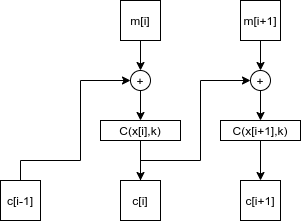
\includegraphics[width = 170pt]{images/CBC.png}
\end{center}
\begin{align*}
	x_{i} = m_{i} \oplus c_{i-1} && c_{i} = C(m_{i} \oplus c_{i-1}, K)
\end{align*}
\noindent questa modalità è detta \emph{Cipher Block Chaining} (CBC).
\paragraph{Decifrazione} La decifrazione invece si esegue in questo modo:
\begin{center}
    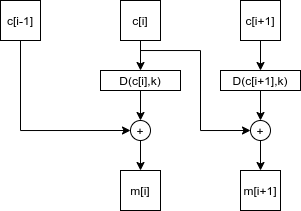
\includegraphics[width = 170pt]{images/CBC_2.png}
\end{center}
$$
    m_i = D(c_i, K) \oplus c_{i-1}
$$
\paragraph{Osservazione} Mentre la cifratura va eseguita necessariamente sequenzialmente (visto che un elemento dipende dal precedente) la decifratura si può eseguire in parallelo (abbiamo tutti gli elementi, non dobbiamo attendere il precedente).
Inoltre se invio il testo cifrato e ci sono errori risulta in un errata decifrazione solo del blocco $i$ e $i+1$ mentre gli altri continuano ad essere decriptati correttamente.

	\part{Crittografia a chiave pubblica}
\chapter{Introduzione}
\section{Problema base: scambio delle chiavi su canali insicuri}
Abbiamo visto che il One-Time Pad è assolutamente sicuro, ma:
\begin{itemize}
	\item richiede una chiave segreta nuova per ogni messaggio;
	\item la chiave deve essere perfettamente casuale e lunga come il messaggio da cifrare.
\end{itemize}
AES ha chiavi più corte, ma necessita comunque di uno scambio di chiavi. Segue la domanda: come si può scambiare una chiave in maniera sicura? La cosa può essere risolta in due modi:
\begin{itemize}
	\item protocollo Diffie-Hellman;
	\item crittografia a chiave pubblica.
\end{itemize}
\paragraph{Protocollo Diffie-Hellman (DH)}
Nel 1976 Diffie ed Hellman con il loro articolo \emph{New Directions in Cryptography} hanno rivoluzionato la crittografia.
Il protocollo \emph{DH} (Diffie-Hellman) permette la negoziazione di una chiave di sessione senza che le due parti si siano scambiate informazioni in precedenza.
\section{Schema della crittografia a chiave pubblica}
In parallelo sempre gli stessi Diffie ed Hellman propongonono lo schema di crittografia a chiave pubblica, senza tuttavia averne una valida implementazione. 
\paragraph{Chiavi} In questo nuovo schema si hanno due chiavi:
\begin{itemize}
    \item una \emph{pubblica} nota a tutti ed utilizzata per cifrare
    \item una \emph{privata}  nota solo al ricevente usata per decifrare
\end{itemize}
Ogni utente avrà quindi una coppia $ <K_{priv}, K_{pub}>$: l'utente rende nota la chiave pubblica e mantiene riservata quella privata. Abbiamo $2N$ chiavi in totale (dove $N$ è il numero di utenti, in contrasto con le $N^2$ chiavi richieste in un cifrario simmetrico).

\paragraph{Funzione di cifratura e decifrazione} La cifratura ha la forma:
$$ c = C(m, K_{pub}) $$
mentre la decifrazione ha la forma:
$$ m = D(c, K_{priv})$$
Entrambe le funzioni sono note al pubblico, così come le chiave pubblica. La chiave privata è nota al solo destinatario, dunque solo il destinatario è in grado di decifrare il messaggio.

\paragraph{Asimmetricità} Il cifrario si dice asimmetrico perché le due parti hanno ruoli diversi, in particolare non c'è più la condivisione di un segreto comune. 

\subsection{Caratteristiche del cifrario}
Questi cifrari devono avere alcune caratteristiche:
\begin{itemize}
    \item \textbf{il procedimento di cifratura e decifrazione deve essere corretto}, il destinatario deve poter risalire al messaggio in chiaro
    $$D(C(m, K_{pub}), K_{priv}) = m$$
    \item \textbf{il sistema deve essere efficiente e sicuro}, cioè 
    \begin{itemize}
    	\item la coppia di chiavi deve essere facile da generare, e deve risultare praticamente impossibile che due utenti scelgano la stessa chiave pubblica (altrimenti la chiave privata risulterebbe la stessa);
    	\item dato un messaggio $m$ e la chiave pubblica $K_{pub}$ deve essere facile per il mittente calcolare il crittogramma
    	\item dato un crittogramma $c$ e la chiave privata $K_{priv}$ deve essere facile per il destinatario calcolare il messaggio orginale
    	\item pur conoscendo il crittogramma $c$, la chiave pubblica $K_{pub}$ e le funzioni di cifratura e decifrazione, deve essere difficile per il crittoanalista risalire a $m$. 
    \end{itemize}
\end{itemize}
I due requisiti elencati possono essere soddisfatti ricorrendo alle \emph{funzioni one-way trap-door}, funzioni facili da calcolare ma \textbf{difficili da invertire} senza avere maggiori informazioni.
\paragraph{RSA} Nel 1977 Rivest, Shamir ed Adleman scoprono una funzione di questo tipo basata sui numeri primi.
L'algoritmo RSA (\textit{Rivest-Shamir-Adleman}) si basa sul fatto che 
\begin{itemize}
	\item dati due numeri primi $p$ e $q$ calcolare il prodotto $n = p \cdot q$, mentre
	\item dato $n$ è difficile fare la fattorizzazione per trovare $p$ e $q$ (a meno che non si conosca uno dei due fattori).
\end{itemize}
\[\boxed{\text{Prima di introdurre l'RSA è necessario introdurre nozioni di algebra modulare.}}\]

\subsection{Vantaggi e svantaggi}
\begin{itemize}
	\item \textbf{Pro}:
	\begin{itemize}
		\item meno chiavi
		\item \textbf{\underline{non richiedono lo scambio di chiavi}} (si risolve problema tipico della crittografia simmetrica)
	\end{itemize}
	\item \textbf{Con}:
	\begin{itemize}
		\item più lenti della cifratura simmetrica
		\item esposizione ad attacchi \textit{chosen plain-text} 
		
		Si può infatti criptare un tot di messaggi $m_1, \dots, m_h$ e vedere se sul canale passa uno dei vari $c_1, \dots, c_h$. Se compare allora sappiamo il messaggio, se non compare allora sappiamo quale messaggio sicuramente non è.
	\end{itemize}
\end{itemize}
Adotteremo un ibrido tra crittografia a chiave pubblica e cifrari simmetrici.
%\subsection{Cifrari ibridi}
%\begin{itemize}
%	\item La crittografia a chiave pubblica risolve il problema dello scambio delle chiavi. Normalmente si utilizza per scambiare la chiavi (trasmissione lenta).
%	\item Ciò che si usa per criptare il messaggio è l'AES (trasmissione veloce).
%	\item L'attacco\textit{ chosen plain-text} è risolto con chiavi random difficilmente prevedibili. 
%	\item La chiave pubblica va estratta da un certificato digitale per evitare attacchi man-in-the-middle in cui terzi si spacciano per il destinatario.
%\end{itemize}
\[\boxed{\text{Si legga le nozioni di Algebra modulare in fondo alla dispensa prima di proseguire.}}\]
\section{Generatori}
Sia data la seguente funzione
$$ a^k \text{ mod } n $$
con $a \in Z_{n}^*$ e $1 \leq k \leq \phi(n)$. Si dice che $a$ è un \emph{generatore di $Z_{n}^*$} se la funzione genera \textbf{\underline{{tutti e soli}}} gli elementi di $Z_{n}^*$.
\paragraph{Ordine degli elementi} L'ordine degli elementi è difficile da prevedere. L'unica cosa prevedibile è che $1$ si ottiene \textbf{\underline{solo}} quando $$x = \phi(n)$$ poiché sappiamo $a^{\phi(n)} \equiv 1 \mod n$ per il teorema di Eulero.  
\paragraph{Esempi}
\begin{itemize}
	\item $2$ è generatore di $Z_{13}^*$
	$$Z_{13}^*=\{1,2,3,4,5,6,7,8,9,10,11,12\}\,\,\,\,\phi(13)=12$$
	$$2^k \text{ mod } 13=2,4,8,3,6,12,11,9,5,10,7,1\,\,\,\,\,\,\,\,\,\,1\leq k \leq 13$$
	\item $3$ è generatore di $Z_7^*$ 
	$$Z_7^*=\{1,2,3,4,5,6\}\,\,\,\,\phi(7)=6$$
	$$3^k \text{ mod } 7=3,2,6,4,5,1\,\,\,\,\,\,\,\,\,\,1\leq k \leq 6$$
	\item $2$ non genera $Z_7^*$
	$$2^3 \text{ mod } 7 = 2^6 \text{ mod }7=1$$
	facendo le potenze con modulo otteniamo $1$ generato per valori diversi da $\phi(n)$, e questo non va bene!
\end{itemize} 
\subsection{Teorema sull'esistenza di almeno un generatore} 
\[\text{Se $n$ è primo allora $Z_{n}^*$ ha almeno un generatore.}\]
\begin{itemize}
	\item \textbf{{Non tutti gli elementi sono generatori}}.\\Per $n$ primo non tutti gli elementi di $Z_n^*$ sono suoi generatori (1 non lo è mai).
	\item \textbf{Numero di generatori}. Per $n$ primo i generatori di $Z_n^*$ sono $\phi(n-1)$.
\end{itemize}
\paragraph{Numeri non primi} Non tutti gli $n$ forniscono generatori per $Z_{n}^*$, ad esempio $Z_8^*$.

\subsection{Problema: individuare i generatori}
Determinare un generatore di $Z_n^*$ con $n$ primo è difficile, si possono provare tutti i numeri in $[2, n-1]$ ma è esponenziale nella dimensione di $n$. Esistono tuttavia algoritmi randomizzati che risolvono il problema con altissima probabilità di successo.

\subsubsection{Problema del logaritmo discreto}
Il calcolo consiste nel trovare $x$ che risolve:
$$ a^x \equiv b \text{ mod } n, \text{n primo} $$
L'equazione ammette soluzioni $\forall b$ se e solo se $a$ è un generatore di $Z_n^*$. Tuttavia non possiamo sapere in che ordine sono generati i valori di $Z_n^*$ quindi per trovare $x$ giusto dobbiamo iterare tutti i valori. 

\paragraph{Rendiamo chiara l'idea} L'algebra modulare complica le cose. Prendiamo la potenza $2^x$: nell'algebra modulare si perde struttura, e quindi la possibilità di costruire algoritmi efficienti.
\begin{table}[ht!]
	\centering
	\small
	\begin{tabular}{c|c c c c c c c c c c c c}
		$x$ & 1 & 2 & 3 & 4 & 5 & 6 & 7 & 8 & 9 & 10 & 11 & 12  \\
		\hline
		$2^{x}$ & 2 & 4 & 8 & 16 & 32 & 64 & 128 & 256 & 512 & 1024 & 2048 & 4096  \\
		$2^{x} \text{ mod } 13$ & 2 & 4 & 8 & 3 & 6 & 12 & 11 & 9 & 5 & 10 & 7 & 1  \\
	\end{tabular}
\end{table}
\begin{itemize}
	\item \textbf{Esempio dall'algebra NON modulare}.
	
	Sappiamo che
	$$2^x=512$$
	e vogliamo trovare $x$. Supponiamo che la soluzione sia $x=8$: facendo i calcoli ci rendiamo conto di avere sbagliato. La cosa non è vana perchè otteniamo informazioni: osservo che $2^8 = 256$, quindi è stato scelto un numero $x$ troppo basso (escludo i valori minori di otto). Provo i numeri maggiori: con $x=9$ otteniamo $512$!
	
	\item \textbf{Esempio nell'algebra modulare}.
	
	Sappiamo che
	$$2^x \text{ mod } 13 = 5$$
	e vogliamo trovare $x$. L'assenza di struttura ordinata mi impedisce di ottenere informazioni dopo aver compiuto errori. Poniamo $x=6$
	$$2^6 \text{ mod } 13 = 12$$
	il risultato non è giusto, ma contrariamente a prima non posso escludere i valori di $x$ minori o quelli superiori: devo provarli per forza tutti! A un certo punto troveremo che la soluzione è $x=9$.
	
\end{itemize}

\section{Funzioni \textit{one-way trap-door}}
Le funzioni \emph{one-way trap-door} permettono la ostruzione di cifrari a chiave pubblica: 
\begin{itemize}
	\item \emph{one-way} in quanto funzioni facili da calcolare, ma difficili da invertire
	\item \emph{trap-door} per la possibilità di calcolare l'inverso in presenza di alcune informazioni
\end{itemize} 

\subsection{Esempio: problema della fattorizzazione} Dati $p, q$ primi è facile fare il prodotto
$$ n = p \cdot q$$
Non possiamo dire la stessa cosa se dato $n$ vogliamo trovare $p$ e $q$: è necessario tempo (sub)esponenziale. 
\paragraph{Trapdoor} Dato $p$ o $q$, invece, si fattorizza velocemente: $q = \frac{n}{p}$, ma anche conoscendo $\phi(n)$ si fattorizza velocemente. Lo si può fare in O($\log_2z$).
\paragraph{RSA} Questo problema determina la "robsutezza" del cifrario RSA.

\subsection{Esempio: calcolo della radice in modulo}
Abbiamo visto che è sufficiente tempo polinomiale per trovare $y$ (algoritmo delle quadrature successive)
$$y = x^z \text{ mod } s $$
Se $s$ non è primo, tuttavia, calcolare la base $x$ (distinguere dal problema del logaritmo discreto, dove si va a calcolare l'esponente e non la base) richiede tempo esponenziale $$x = y^{\frac{1}{z}} \text{ mod } s$$ 
\paragraph{Applicazioni} Tutte le volte che chiediamo due interi primi $p$ e $q$ andiamo a calcolare un valore $n$ non primo.
n 
\paragraph{Attenzione} Parliamo del calcolo della radice in modulo, non del calcolo della radice e basta! Il calcolo della radice senza modulo è facile da calcolare (si osservi che nell'RSA si deve stare attenti a non avere $m<n$ con $m \text{ mod } n$)



\paragraph{}
	\chapter{RSA (Rivest-Shamir-Adleman)}
\section{Generazione delle chiavi}
La creazione della coppia di chiavi spetta al destinatario.
\begin{enumerate}
    \item Si scelgono due numeri interi e primi $p$, $q$ molto grandi ($\approx 1000$ bit) (adesso si consiglia che $p \cdot q \approx 2048$ bit per avere una protezione fino al 2030, mentre per una protezione di maggiore durata si consigliano 3072 bit). Ovviamente questo passo deve essere fatto in tempo polinomiale (la generazione di $p$ e $q$): si generano sequenze casuali (nei modi già visti) e \textbf{\underline{si testa la primalità utilizzando il test di Miller-Rabin}}.
    \item Si calcola il prodotto $n$ e la funzione di Eulero $\phi(n)$ (questo è facile da calcolare, poichè conosciamo la scomposizione di $n$, si ricordi la formula vista indietro)
    \begin{align*}
    	n&=p\cdot q\\
    	\phi(n)&=(p-1) \cdot (q-1)
   \end{align*}Anche qui operazioni in tempo polinomiale nella grandezza dell'input.
    \item Si sceglie $e < \phi(n)$ tale che $e$ e $\phi(n)$ siano coprimi
    $$\text{MCD}(e, \phi(n))=1$$
    \item Si calcola $$d = e^{-1} \text{ mod } \phi(n)$$ Anche questo si può calcolare in tempo polinomiale usando l'algoritmo di Euclide esteso. Si osservi che essendo $MCD(e, \phi(n))=1$ si ha unicità della soluzione ($e^{-1}$).
\end{enumerate}

\paragraph{Risultato finale} Alla fine si hanno quindi le due chiavi:
\begin{align*}
K_{pub} = <e,n> && K_{priv} = <d,n>
\end{align*}
Naturalmente va tenuto segreto anche il resto delle informazioni: $p$, $q$, $\phi(n)$.

\section{Cifratura e decifratura}
\[\boxed{\text{I messaggi sono sequenze binarie trattate come interi!}}\]
\begin{itemize}
	\item  \textbf{NB}. Indichiamo il messaggio $m$ e imponiamo $m<n$. In caso contrario potrebbero emergere ambiguità nella decifrazioni: la cosa è chiara nella dimostrazione di correttezza, non sarà possibile arrivare a conclusione senza adottare questa condizione. Se $m \geq n$ allora dividiamo il messaggio $m$ in blocchi di $b = \lfloor \log_2n \rfloor$ bit (sempre con la stessa chiave) e cifriamo ciascuno (eventualmente con CBC).
	\item \textbf{NB2}. Solitamente si fissa un limite inferiore comune per la dimensione dei blocchi, prevenendo così l'uso di cifrari poco sicuri. Supponiamo che il blocco sia di almeno $b$ bit: i messaggi saranno numeri fino a $2^b$, ma lo stesso massimo deve essere minore di $n$ per la condizione detta $$m < 2^b < n$$ 
	\item \textbf{Cifratura}. Abbiamo la chiave pubblica $<e,n>$ e il messaggio $m$
	$$ c = C(m, K_{pub}) = m^{e} \text{ mod } n$$
	con $m<n, c <n$
	\item \textbf{Decifrazione}. Abbiamo la chiave privata $<d,n>$ e il crittogramma $c$
	$$ m = D(c, K_{priv}) = c^{d} \text{ mod } n$$
\end{itemize} 
Sicuramente il cifrario RSA è molto elegante! L'utilizzo del modulo garantisce la sicurezza del cifrario. 

\subsection{Esempio}
Consideriamo il seguente esempio.
\begin{enumerate}
	\item Calcoliamo $p,q$ e la funzione di Eulero
	\begin{align*}
		p=5, q= 11 \Longrightarrow \,&n = p \cdot q = 5 \cdot 11 = 55\\
		&\phi(n)=(p-1)\cdot(q-1)=40
	\end{align*}
	\item Scegliamo un valore $e$ coprimo con $40$: prendiamo $e=7$, che è coprimo con $\phi(n)=40$ poichè
	$$\text{MCD}(7,40)=1$$
	\item Applichiamo l'algoritmo di Euclide esteso per calcolare l'inverso moltiplicativo\\$d=7^{-1}\text{ mod }40$
	\begin{verbatim}
	EE(7,40) ---> <1, -17>
	EE(40, 7 mod 40) = EE(40, 7) ---> <1,3,-2 - floor(40/7)*3 = <1,3,-17>
	EE(7, 40 mod 7) = EE(7, 5) ---> <1, -2, 1 - floor(7/5)*(-2)> = <1,-2,+3>
	EE(5, 7 mod 5) = EE(5, 2) ---> <1,1,0 - floor(5/2)*1> = <1,1,-2>
	EE(2, 5 mod 2) = EE(2, 1) ---> <1,0, 1 -  floor(2/1)*0> = <1,0,1>
	EE(1, 0) ---> <1,1,0>
	\end{verbatim}
	L'inverso risultante è $-17$, che è negativo: visto che lavoriamo in modulo $40$ sommiamo $40$. Morale della favola:
	$$d=-17 \text{ mod } 40 = 23 \text{ mod } 40=23$$
	\item Abbiamo ottenuto 
	\begin{align*}
		K_{pub}=<7,55>&&K_{priv}=<23, 55>
	\end{align*}
	Per decifrare faremo ($m< 55$)
	\begin{align*}
		c&=m^7 \text{ mod }55\\m&=c^{23} \text{ mod } 55
	\end{align*}
	Si possono eseguire i calcoli in tempo polinomiale tramite l'algoritmo delle quadrature successive.
\end{enumerate}


\section{Dimostrazione del teorema di correttezza del cifrario}
Dimostrare la correttezza del cifrario significa dimostrare che
$$ D(C(m, K_{pub}), K_{priv}) = m $$
nel contesto del RSA significa dimostrare che ($\forall  m < n$)
$$c^d\text{ mod }n=(m^e \text{ mod } n)^d \text{ mod } n = \boxed{m^{ed} \text{ mod } n = m}$$
%diciamo questo dalla nuova proprietà dell'operatore modulo introdotta qualche pagina fa
%$$a^{r \times s} \text{ mod } m &= (a^r \text{ mod } m)^{s} \text{ mod } m$$
La cosa non è così ovvia: $e$ e $d$ sono l'uno l'inverso dell'altro ma rispetto a mod $\phi(n)$ e non mod $n$ (\textbf{\underline{ricordare come abbiamo generato la chiave}})
$$ed \equiv 1 \text{ mod } \phi(n)$$
La dimostrazione del teorema di correttezza del cifrario si fa affrontando tre casi. Si prenda il prodotto $n=p\cdot q$ e chiediamoci: cosa succede se provo a dividere il messaggio $m$ (che trattiamo come intero) per $q$? Cosa succede se faccio lo stesso con $p$?

\subsection{Caso: il messaggio $m$ è divisibile sia per $q$ che per $p$}
Avere $m$ divisibile sia per $p$ che per $q$ significa che è divisibile per $n$. 
\[\boxed{\text{Ciò non è possibile perché abbiamo imposto $m < n$.}}\]
La divisione risulta possibile solo se $m$ è almeno uguale ad $n$ (e quindi se $m \geq n$).
$\hfill\blacksquare$

\subsection{Caso: $p$ e $q$ non dividono il messaggio $m$}
Se $p$ e $q$ non dividono $m$ allora $m$ ed $n$ sono coprimi, cioè: $\text{MCD}(m,n)=1$. Riprendiamo le seguenti cose.
\begin{itemize}
	\item \textbf{Teorema di Eulero}: $m^{\phi(n)} \equiv 1 \text{ mod }n$ (possiamo dirlo visto che $\text{MCD}(m,n)=1$)
	\item \textbf{Definizione di inverso} (con $r \in \mathbb{N}$): $ed \equiv 1 \text{ mod } \phi(n) \Longrightarrow ed=1+r \cdot \phi(n)$
\end{itemize}
Partendo da quest'ultima cosa scriviamo
$$ m^{ed} \text{ mod } n = m^{1 + r \cdot \phi(n)} \text{ mod } n = m \cdot (m^{\phi(n)})^{r} \text{ mod } n$$
Abbiamo detto che $m$ ed $n$ sono coprimi, \textbf{\underline{quindi possiamo utilizzare il teorema di Eulero}}. 
$$ m \cdot 1^r \text{ mod } n = m \text{ mod } n = m $$
L'ultimo passaggio è certo (la rimozione del modulo) poichè $m <n$
$\hfill\blacksquare$
\subsection{Caso: il messaggio $m$ è divisibile per $p$ e non per $q$ (o viceversa)}
Supponiamo che $m$ e $n$ non siano coprimi: in particolare abbiamo $m$ divisibile per $p$ e non per $q$ (o viceversa). Non possiamo usare il teorema di Eulero come appena fatto! 
\paragraph{Numero  divisibile }Se $p$ è multiplo di $m$ allora
$$m \equiv 0 \text{ mod }p \longrightarrow m \text{ mod }p=0$$
tutte le potenze di $m$ continueranno ad essere divisibili per $p$, quindi
$$\forall r \in \mathbb{N}\,\,\,\,\, \,\,\,m^r\equiv 0 \text{ mod }p \longrightarrow m^r  \text{ mod } p=0$$
siccome sia $m^r$ che $m$ sono congrui a $0$ modulo $p$ allora lo è pure la differenza
$$\forall r \in \mathbb{N}\,\,\,\,\,\,\,\,m^r-m\equiv 0 \text{ mod } p \longrightarrow (m^r-m) \text{ mod } p = 0$$
Possiamo porre $r=ed$
$$m^{ed}-m\equiv 0 \text{ mod } p$$
\paragraph{Numero non divisibile} Ricaviamo una relazione simile anche per $q$. Sappiamo che $q$ ed $m$ sono coprimi, dunque è applicabile il teorema di Eulero
$$m^{\phi(q)} \equiv 1 \text{ mod }q \longrightarrow m^{\phi(q)} \text{ mod } q = 1$$
Facciamo i seguenti calcoli:
\begin{align*}
	m^{ed} \text{ mod } q = m^{\phi(n) \cdot r + 1} \text{ mod } q &= m \cdot m^{r(p-1)\cdot(q-1)} \text{ mod }q=m \cdot (m^{(q-1)})^{(p-1)\cdot{r}} \text{ mod } q=\\&=m \cdot (m^{\phi(q)})^{(p-1)\cdot{r}} \text{ mod } q=m \text{ mod } q\end{align*}
$q$ è numero primo, dunque la funzione di Eulero è il numero decrementato ($\phi(q)=q-1$).  Concludiamo:
$$ m^{ed} \equiv m \text{ mod } q \implies m^{ed} - m \equiv 0 \text{ mod } q $$
\paragraph{Conclusione} Abbiamo quindi ottenuto:
\[
    \begin{cases}
    $$ m^{ed} - m \equiv 0 \text{ mod } q $$ \\ 
    $$ m^{ed} - m \equiv 0 \text{ mod } p $$
    \end{cases}
\]
che significa che $ m^{ed} -m $ è divisibile sia per $p$ che per $q$ quindi lo sarà anche per $n = p \cdot q$, possiamo quindi dire:
$$ m^{ed} -m \equiv 0 \text{ mod } n \Longrightarrow m^{ed} \equiv m \text{ mod } n = m $$
L'ultimo passaggio è certo (la rimozione del modulo) poichè $m <n$
$\hfill\blacksquare$

\section{Sicurezza del cifrario ed attacchi}
\subsection{Soluzioni equivalenti alla fattorizzazione}
La sicurezza è legata alla difficoltà della fattorizzazione di un numero molto grande. 
\[\boxed{\text{La fattorizzazione è C.S. (non si sa se  C.N.) per rompere RSA in tempo polinomiale}}\]
Se fattorizzo $n$ trovo $p$ e $q$, e quindi $\phi(n)=(p-1)(q-1)$. 
Consideriamo le possibili alternative, tutte equivalenti alla fattorizzazione.
\begin{itemize}
	\item \textbf{Calcolo della radice in modulo}. 
	$$m = \sqrt[e]{c} \mod n$$
	Il calcolo è difficile \textbf{\underline{almeno}} quanto la fattorizzazione di $n$ ($n$ composto), non emerge utilità nello svolgere questi calcoli.
	\item \textbf{Calcolo di $\phi(n)$ direttamente da $n$}.
	
	Il calcolo di $\phi(n)$ a partire da $n$ è computazionalmente equivalente alla fattorizzazione di $n$: se io calcolo $\phi(n)$ da $n$ allora conoscendo i due posso trovare $p$ e $q$ in tempo polinomiale. 
	$$\boxed{n = p \cdot q \xrightarrow{} \phi(n) = (p-1) \cdot (q-1)}$$
	Calcoliamo $\phi(n)$
	\begin{align*}
		\phi(n) &= (p-1) \cdot (q-1)= p \cdot q - (p+q) + 1 = n - (p+q) + 1
	\end{align*}
	ottengo $ x_1 = p+q = n - \phi(n) + 1 $, 	poi $ (p-q)^2 = (p+q)^2 - 4 \cdot n = (x_1)^2 - 4 \cdot n $
	
	quindi $ x_2 = p - q = \sqrt{x_1^{2} - 4 \cdot n}$
	
	ottengo che i due problemi sono equivalenti.
	\[
	\begin{cases}
		x_1 = p + q \\ 
		x_2 = p - q
	\end{cases}	\Longrightarrow \begin{cases}
		p = \frac{x_1 + x_2}{2} \\
		q = \frac{x_1 - x_2}{2}
	\end{cases}
	\]
	
	\item \textbf{Attacco esauriente su $d$}. 
	
	Un altro attacco che posso fare è cercare di brutare $d$ partendo da $(n,e)$.
\end{itemize}
\paragraph{NB} Fattorizzare non è \emph{NP-hard} quindi non si esclude che esista un algoritmo efficiente.
\pagebreak 

\subsection{Osservazioni sulla fattorizzazione di n}
La fattorizzazione è difficile, ma non più come una volta: l'hardware migliora e gli algoritmi si affinano (pur rimanendo costosi sul piano computazionale). Non è definito un limite inferiore: questo significa che in futuro potrebbero emergere algoritmi aventi migliore complessità.
\begin{itemize}
    \item Esistono algoritmi di \textbf{complessità sub-esponenziale} come il \emph{General Number Field Sieve} (GNFS) che richiede O($2^{\sqrt{b \cdot \log b}}$) con $b$ la dimensione di $n$ (un attacco brute-force è O($2^b$)).
    \item Con la potenza di calcolo attuale usando GNFS si fattorizza fino a 768 bit. Nuovi algoritmi hanno ridotto il numero di bit di sicurezza, ergo hanno comportato un aumento del numero di bit necessari per garantire la sicurezza. Per avere una sicurezza come quella che si ottiene con AES a 128 bit si dovrebbe ricorrere a $n$ con circa 3072 bit, si sale addirittura a 15360 bit di modulo se lo si compara con AES256.
    \begin{center}
    	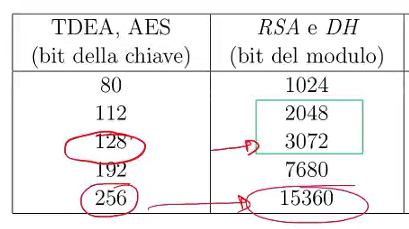
\includegraphics[scale=.8]{images/25.PNG}
    \end{center}
    Nell'AES i bit della chiave sono tutti bit di sicurezza, mentre nel RSA i bit del modulo non sono tutti di sicurezza: \textbf{si hanno attacchi più efficienti del forza bruta} (motivo per cui nel tempo i bit aumentano).
\end{itemize}

\subsection{Scelta ottimale dei valori $p,q$}
I numeri $p$ e $q$ vanno scelti \emph{molto} grandi, \emph{entrambi} attorno ai 1700 bit: se uno è troppo piccolo la fattorizzazione ci mette poco a individuare il numero piccolo.
\begin{itemize}
	\item Sia $p-1$ che $q-1$ devono contenere fattori grandi (altrimenti $n$ si fattorizza velocemente).
	\item $\text{MCD}(p-1, q-1)$ deve essere piccolo! Conviene scegliere $p$ e $q$ tali che i numeri $\frac{p-1}{2}$ e $\frac{q-1}{2}$ siano coprimi.
	\item \textbf{Norma di buon senso: cambiare sempre entrambi i numeri primi}.
	
	Mai riutilizzare uno dei primi per altri moduli: il crittoanalista potrebbe pensare che io per pigrizia ho generato un nuovo numero primo mantenendo l'altro numero primo. La cosa non è un problema, sappiamo ottenere i numeri primi in tempo polinomiale.
	\[\begin{cases}
			n_1 = p \cdot q_1 \\
			n_2 = p \cdot q_2
		\end{cases}
		\implies \text{MCD}(n_1, n_2) = p
	\]

\item \textbf{Attacco con $p$ e $q$ simili}.

Scegliere $p$ e $q$ distanti tra loro! Se $p \approx q$ allora si ha un attacco molto efficiente dove si ipotizza $$n \approx q^2 \approx p^2$$
quindi $p \approx \sqrt{n}$ e si cerca nell'intorno della radice di $n$. Valgono infatti:
$$ \left(\frac{p+q}{2}\right)^2 -n = \left(\frac{p-q}{2}\right)^2 $$
\begin{itemize}
	\item Mi dice che $\frac{p+q}{2} > \sqrt{n}$ perché $\left(\frac{p-q}{2}\right)^2> 0$ sempre, se $p \neq q$.
	
	\item Inoltre $\frac{(p+q)^2}{4}-n$ è un quadrato perfetto: $(\frac{p-q}{2})^2$.
\end{itemize}
Posso quindi cercare tra gli interi maggiori di $\sqrt{n}$ fino a trovare $z$ tale che $z^2 - n$ sia un quadrato perfetto. Poniamo
$$z^2-n=w^2$$
La soluzione non è unica, dunque dobbiamo fare diversi controlli e verificare se i numeri trovati effettivamente fattorizzano $n$.

Supponiamo dunque di averli trovati, otteniamo: 
\[
	\begin{cases}
		z = \frac{p+q}{2} \\
		w = \frac{p-q}{2}
	\end{cases}
	\Longrightarrow 
	\begin{cases}
		p = z+w \\
		q = z-w
	\end{cases}
\]
La differenza è grande quando cresce come una potenza di $n$, deve crescere più di un logaritmo.
\end{itemize}

\subsection{Attacchi con esponenti ($d$ ed $e$) bassi}
Valori di $e$ e $d$ bassi portano ad accelerare nell'algoritmo, tuttavia se $d$ è piccolo sono possibili attacchi forza bruta.
\paragraph{Problema} Se $m$ è piccolo ed anche $e$ lo è, può succedere che $m^e < n$ quindi non ci sia la riduzione in modulo. In tal caso decripto semplicemente calcolando $\sqrt[e]{m}$.

\subsection{Attacchi a tempo}
\[\boxed{\text{Ne soffre sia RSA che DH.}}\]
Si basano sul tempo di esecuzione dell'algoritmo di decifrazione. Si può quindi determinare $d$ analizzando il tempo impiegato per decifrare.
\begin{itemize}
	\item Nell'algoritmo delle quadrature successive infatti si esegue una moltiplicazione ad ogni iterazione più una ulteriore moltiplicazione modulare per ciascun bit uguale ad 1 in $d$.
	\item Guardando il tempo quindi si può stimare il numero di bit ad 1 in $d$.
	Si può risolvere aggiungendo un ritardo casuale alla fine.
\end{itemize}



\subsection{Attacchi sulla scelta di $e$}
Abbiamo già detto che un valore $e$ troppo basso comporta il rischio di avere $m^e < n$ e quindi
$$m^e \text{ mod } n = m$$
Generalizzando affermiamo che il problema non si manifesta se 
$$ e \neq \frac{\phi(n) + k}{k} $$
per ogni valore $k$ che divide $p-1$ e $q-1$ (\textbf{\underline{ENTRAMBI}}, attenzione al refuso sul libro di Crittografia), con $m$ ed $n$ coprimi.
\paragraph{Attacco con $e$ troppo piccolo} 
\begin{itemize}
	\item Un altro attacco possibile se $e$ è troppo piccolo:
	\begin{itemize}
		\item supponiamo che ci siano $e$ utenti che hanno scelto lo stesso valore piccolo di $e$
		\item gli $e$ utenti ricevono lo stesso messaggio $m$
	\end{itemize}
	Otteniamo il seguente sistema
	\[
	\begin{cases}
		c_1 = m^e \text{ mod } n_1 \\
		c_2 = m^e \text{ mod } n_2 \\
		... \\
		c_e = m^e \text{ mod } n_e \\
	\end{cases}
	\]
	sarà quindi vero che $m < n_i, \forall i \in [1,e]$. 
	
	\item \textbf{Teorema cinese del resto} (da un video di \emph{Alessandro Zaccagnini}). 
	
	Supponiamo di avere un sistema del genere, con $n_1$ ed $n_2$ coprimi
	\[\begin{cases}x  \text{ mod } n_1=a_1 \\x \text{ mod } n_2 = a_2l'ann\end{cases}\]
	abbiamo un'unica soluzione in modulo $n=n_1\cdot n_2$ qualunque siano gli interi $a_1$ e $a_2$.
	\item Ipotiziamo che $n_1,n_2,\dots,n_e$ siano coprimi tra loro (se non lo fossero si potrebbe fattorizzarne qualcuno usando il $MCD$), per il \textbf{teorema cinese del resto} sono certo dell'esistenza di un valore $m'$ tale che:
	\[
	\begin{cases}
		m' < n = n_1 \cdot n_2 \cdot ... \cdot n_e \\
		m' \equiv m^e \text{ mod } n
	\end{cases}
	\]
	Dato che $m < n_i, \forall i$ so che $m \cdot m \cdot ... \cdot m = m^e < n_1 \cdot n_2 \cdot ... \cdot n_e = n$.
	Quindi la riduzione in modulo non avviene e posso calcolare $m = \sqrt[e]{m'}$.
	\item Se voglio continuare ad usare $e$ piccolo posso aumentare la dimensione di $m$ introducendo un \textit{padding} casuale, diverso per ogni utente (messaggi non più uguali).
\end{itemize}

\subsection{Attacco con lo stesso valore di $n$ (\emph{common modulus})}
Supponiamo che due utenti abbiano generato una chiave pubblica con lo stesso $n$ ma diversi $e$:
$$ <e_1,n>, <e_2,n> $$
Supponiamo inoltre che $\text{MCD}(e_1, e_2) = 1$ allora $$\exists r,s \in \mathbb{Z}: e_1 \cdot r + e_2 \cdot s = 1$$ utilizziamo Euclide esteso poichè abbiamo la forma $a\cdot x +b\cdot y = \text{MCD}(a,b)$. Saranno allora $r<0$ e $s>0$. Si intercetta $c_i = m^{e_i} \mod n$ e si voglia trovare $m$:
\begin{align*}
	m = m^1 = m^{r \cdot e_1 + s \cdot e_2 } &= (m^{e_1} \text{ mod } n)^{r} \cdot (m^{e_2} \text{ mod } n)^{s} =\\
	&= (c_1^r \cdot c_2^s) \text{ mod } n = ((c_1^{-1})^{-r} \cdot c_2^s) \text{ mod } n\textbf{}
\end{align*}
Si calcola quindi $c_1^{-1} \mod n$ che esiste se $c_1$ ed $n$ sono coprimi (se non lo fossero potremmo fattorizzare $n$). Se non sono coprimi calcola $m = (c_1^{-1})^{-r} \cdot (c_2)^{s} \text{ mod } n$ in tempo polinomiale.

\section{Cifrari ibridi: uso di RSA ed AES insieme}
Il principale scopo della crittografia a chiave pubblica è quello di scambiare le chiavi! Supponiamo che Alice e Bob vogliano parlare tra di loro in maniera sicura...
\begin{itemize}
    \item \textbf{Alice}: 
    \begin{itemize}
        \item sceglie una chiave AES $k[\text{session}]$  (detta \emph{chiave di sessione}) e la cifra con la chiave pubblica di Bob
        \item cifra il messaggio con $k[\text{session}]$ col cifrario AES
        \item invia i due crittogrammi a Bob (il messaggio cifrato in AES e la chiave cifrata in RSA con la chiave pubblica di Bob).
        $$\left<C_{\text{RSA}}(k[\text{session}], k_{\text{BOB}}[\text{pub}]), C_{\text{AES}}(m, k[\text{session}])\right>$$
    \end{itemize}
    \item \textbf{Bob}:
    \begin{itemize}
    	\item decifra il primo crittogramma con  $k_{\text{BOB}}[\text{priv}]$, ottenendo così $k[\text{session}]$
    	\item decifra il secondo crittogramma utilizzando $k[\text{session}]$
    \end{itemize} 
\end{itemize}

\paragraph{NB} Al termine della sessione la chiave AES va cancellata. Per ogni nuova sessione di comunicazione va creata una nuova chiave (ad ogni messaggio la cosa è troppo impegnativa).

\paragraph{Problema} Un problema di questo approccio è che l'onere di creare la chiave di sessione sta ad Alice. Bob non può essere sicuro che la chiave sia stata generata in modo corretto (creare una chiave rispettando tutti i principi detti richiede risorse)!
In genere sarebbe preferibile porre ambo le parti sullo stesso livello. Risolviamo la cosa introducendo il protocollo \emph{Diffie-Hellman}.

	\chapter{Protocollo Diffie-Hellman}
\section{Spiegazione}
\[\boxed{\text{Non è un cifrario, è solo un protocollo per lo scambio della chiave}}\]
Questo protocollo permette la creazione di una chiave di sessione nella quale entrambi i lati partecipano in egual misura. Non è un protocollo di scambio di chiavi, la chiave non viaggia mai: si scambiano informazioni che permettono la costruzione della chiave (ogni volta si mettono insieme informazioni private di un interlocutore). Il protocollo ricorre all'algebra modulare e basa la sua sicurezza sul problema del logaritmo discreto.
\paragraph{Passi} 
\begin{itemize}
	\item \textbf{Primo step}. Alice e Bob si accordano pubblicamente su un numero $p$ primo molto grande ($\approx 1000$ bit) ed un generatore $g$ di $Z_p^*$. Ricordiamo che
	$$Z_p^*=\{1,2, \dots, p-1\}$$
	che posso esprimere nel seguente modo, grazie al generatore $g$
	$$Z_p^*=\{g^k \text{ mod }p, 1 \leq k \leq p-1\}$$
	Ricordarsi che lavorare con un numero primo garantisce l'esistenza di \textbf{\underline{ALMENO}} un generatore di $Z_p^*$
	\item \textbf{Individuazione del generatore}. Non esistono algoritmi deterministici per individuare generatori (si usano algoritmi randomizzati). Nel caso in cui Alice e Bob non abbiano la potenza computazionale per ottenere $<g,p>$ allora utilizzeranno coppie note, per esempio quelle raccomandate dalle linee guida del NIST: vedremo che ciò non è un problema, nella dimostrazione della correttezza supporremo che la coppia sia nota al crittoanalista.
	\item \textbf{Step successivi}. L'algoritmo prosegue un questo modo:
	\begin{itemize}
		\item Alice sceglie $x$ tale che $1 < x < p-1$ e calcola
		$$ A = g^x \text{ mod } p $$
		ed invia $A$ a Bob
		\item Bob sceglie $y$ tale che $1 < y < p-1$ e calcola
		$$ B = g^y \text{ mod } p $$
		ed invia $B$ ad Alice
		\item Alice calcola la chiave di sessione:
		$$ K = B^x \text{ mod } p = \boxed{g^{x \cdot y} \text{ mod } p} $$
		\item Bob calcola la chiave di sessione:
		$$ K = A^y \text{ mod } p = \boxed{g^{x \cdot y} \text{ mod } p} $$
	\end{itemize}
	Entrambi hanno ottenuto lo stesso numero $K$.
	
\end{itemize}
\section{Sicurezza del problema del logaritmo discreto}
\subsection{Attacchi passivi}
Il crittoanalista conosce il numero primo $p$, il generatore $g$, i valori $A$ e $B$.
Per calcolare la chiave di sessione $k[\text{session}]$ bisogna trovare $x$ ed $y$:
\[
    \begin{cases}
    A = g^x \text{ mod } p \\
    B = g^y \text{ mod } p
    \end{cases}
\]
siamo di fronte al problema del \textbf{logaritmo discreto}! Possiamo solo eseguire un forza bruta ma se $p$ è molto grande {\underline{allora c'è poco da fare}}.

\subsection{Attacchi attivi}
\begin{center}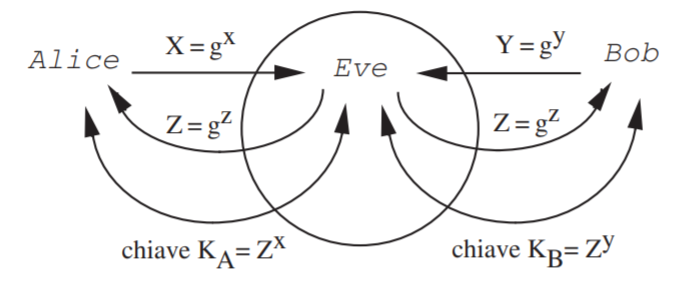
\includegraphics[scale=.6]{images/27.PNG}\end{center}
Diffie-Hellman è vulnerabile agli attacchi di tipo \emph{man-in-the-middle}. Abbiamo Eve che si finge Alice agli occhi di Bob e Bob agli occhi di Alice:
\begin{itemize}
    \item Alice invia $ A = g^x \text{ mod } p$. Eve intercetta $A$ e lo sostituisce con $$E = g^z \text{ mod } p$$
    Bob riceve $E$.
    \item Bob invia $ B = g^y \text{ mod } p $. Eve intercetta $B$ e lo sostituisce con $$E = g^z \text{ mod } p$$
    Alice riceve $E$.
    \item Eve calcola:
    \begin{itemize}
        \item $K_A = A^z \text{ mod } p = g^{x \cdot z} \text{ mod } p$ per parlare con Alice
        \item $K_B = B^z \text{ mod } p = g^{y \cdot z} \text{ mod } p$ per parlare con Bob
    \end{itemize}
    \item Alice calcola $K_A = E^x \mod p$ per parlare con Bob, ma in realtà parlerà con Eve
    \item Bob calcola $K_B = E^y \mod p$ per parlare con Alice, ma in realtà parlerà con Eve
\end{itemize}
Qualsiasi cosa che Alice mandi a Bob, Eve può decifrarlo, criptare con la chiave di Bob e re-inviarlo.
Viceversa per i messaggi di Bob verso Alice.
Eve può quindi leggere tutti i messaggi da ambo le parti. 
\paragraph{Soluzione} Per risolvere questo problema si possono usare le \emph{Certification of Authority}, cioè dei certificati digitali con il quale si firmano i valori $A$ e/o $B$.


	\chapter{Cifrario di El Gamal}
\section{Spiegazione}
Il cifrario di El Gamal è un'alternativa al binomio RSA-AES.
\begin{framed}\noindent \textbf{Costruzione della chiave pubblica}. Bob mette a disposizione la sua chiave pubblica, la costruisce:
	\begin{itemize}
		\item sceglie $p$ molto grande, primo e sceglie $g$ generatore di $Z_p^*$
		\item \textbf{Scelta della chiave privata}. Bob sceglie $x$ tale che $1 < x < p-1$. Sarà la chiave privata $k[\text{priv}]=x$, usata da Bob al momento della decifrazione.
		\item calcola $y = g^x \text{ mod } p$
		\item ha ottenuto $k[\text{pub}]=<p, g, y>$
	\end{itemize}
\end{framed}
\paragraph{Cifratura} Alice vuole inviare un messaggio $m$ a Bob.
\[\boxed{\text{Il messaggio è trattato come un numero tale che: $0 \leq m < p$.}}\]
\begin{itemize}
    \item Si procura la chiave pubblica di Bob $k[\text{pub}]=<p, g, y>$ 
    
    \item Sceglie a caso $1 < r < p-1$ (da tenere segreto)
    \item Calcola $c$ e $d$
    \begin{align*}
    	c = g^r \text{ mod } p&&d = m \cdot y^r \text{ mod } p
    \end{align*}
	$c$ apparterrà a $Z_p^*$, ovviamente. 
    \item Allo step precedente Alice ha  ottenuto la coppia $<c,d>$, che invia a Bob. \begin{itemize}
    	\item $c$ contiene "protetto" l'informazione sul numero casuale $r$ (protetto perchè c'è il problema del logaritmo discreto se volessi calcolare $r$)
    	\item $d$ è il messaggio $m$ a cui è stata applicata una maschera (messaggio trattato come un numero, moltiplicato per un valore casuale)
\end{itemize}\end{itemize}
\paragraph{Decifrazione} Bob deve quindi decifrare il messaggio:
$$ m = \frac{d}{c^x} \text{ mod } p = d\cdot \frac{1}{c^x} \text{ mod } p= d \cdot c^{-x} \text{ mod } p $$
$x$ è la chiave privata scelta da Bob! Il calcolo è possibile solo se si conosce la chiave privata.

\section{Dimostrazione di correttezza}
Per dimostrare la correttezza recupero la formula con cui Alice ha calcolato $d$ e $c$, e la formula con cui Bob ha calcolato $y$.
$$ \frac{d}{c^x} \text{ mod } p = \frac{y^r \cdot m}{c^x} \text{ mod } p = \frac{\cancel{(g^x)^r} \cdot m}{\cancel{(g^r)^x}} \text{ mod } p = m $$
E' sicuro perché Eve conosce $<p,g,y,c,d>$, tutto tranne $r$ ed $x$: conoscere almeno una delle due cose permetterebbe di trovare il messaggio in chiaro $m$.
\paragraph{Trapdoor} 
\begin{itemize}
	\item Se si conoscesse $x$ si potrebbe calcolare $$m = \frac{d}{c^x} \text{ mod } p$$
	\item Se si conoscesse $r$ si potrebbe calcolare $$m = \frac{d}{y^r} = \frac{\cancel{y^r} \cdot m}{\cancel{y^r}} \text{ mod } p$$
\end{itemize}
\paragraph{NB} Importante mantenere $r$ segreto ed usarlo solo una volta!
	\chapter{Crittografia su curve ellittiche}
Attorno al 1985 Miller (IBM, non lo stesso Miller di Miller-Rabin) e Koblitz (University of Washington) propongono di prendere RSA e DH e cambiare le operazioni in algebra modulare con operazioni su curve ellittiche.
\paragraph{Wait} Prima di introdurre il cifrario è necessario entrare nel concetto di \emph{curva ellittica}.

\section{Vantaggi della crittografia a curve ellittiche}
Si sta via via abbandonando la crittografia basata sull'algebra modulare per abbracciare operazioni definite sui punti di una \emph{curva ellittica}: 
\begin{itemize}
	\item le chiavi risultano più piccole a parità di sicurezza;
	\item fattorizzazione e logaritmo discreto si risolvono in tempi sub-esponenziali.
\end{itemize}
Gli algoritmi per rompere la cifratura su curve ellittiche rimangono ad ora ancora esponenziali puri (anche qua vale l'approccio delle funzioni \emph{one-way trap-door}).
\begin{table}[ht]
    \centering
    \begin{tabular}{c|c|c}
        AES & RSA, DH, El Gamal & ECC \\
        \hline
        128 bit & 3072 bit ($n$ per RSA, $p$ per DH) & 256 bit \\
        256 bit & $\approx 15'000$ bit & 512 bit
    \end{tabular}
\end{table}

\noindent Il fatto è che ECC ECC (\emph{Elliptic Curve Cryptography}) offre la stessa sicurezza di RSA, ma con un numero di bit decisamente inferiore! Logicamente ci piace di più un cifrario che richiede una minore occupazione di memoria.

\section{Curve ellittiche}
\paragraph{Definizione di campo} \emph{Il campo $K$ è un insieme non vuoto dotato di operazioni binarie interne, chiamate addizione e sottrazione, che soddisfano la proprietà associativa, commutativa, di esistenza dell'elemento neutro e di esistenza dell'inverso di ciascun elemento (ad eccezione dello zero per la moltiplicazione)}. 
\paragraph{Forma generale} Preso un campo $K$ una curva ellittica è l'insieme dei punti $(x,y) \in K^2$ tale che:
$$ y^2 + axy + by = x^3 + cx^2 + dx + e $$
con $a,b,c,d,e \in K$.

\paragraph{Definizione di caratteristica del campo} La caratteristica di un campo è il numero di volte per il quale devo sommare l'elemento neutro moltiplicativo $1$ per ottenere l'elemento neutro additivo $0$.
\begin{itemize}
	\item Negli interi modulo $p$ la caratteristica è $p$.
	\item Nei reali la caratteristica è 0 (non esistono numeri in grado di fare quanto detto).
\end{itemize}

\paragraph{Forma normale di Weierstrass} Se la caratteristica di $K \neq 2, 3$ allora esiste una forma semplificata:
$$ y^2 = x^3 + ax + b $$
con $a,b \in K$. Scriviamo quindi:
$$ E_K = \{ (x,y) \in K^2 \mid y^2 = x^3 + ax +b \} \cup \{0\} $$
Si osservi che introduciamo l'elemento neutro $0$ dell'operazione (quella che stiamo costruendo), uniamo all'insieme di punti un elemento 0 che in base al campo può già esistere o meno. Sarà per noi un punto all'infinito.
\paragraph{Gruppo Abeliano} All'interno di $E(a,b)$ possiamo definire una operazione interna, dando all'insieme la struttura algebrica di un \emph{gruppo Abeliano}: ci limitiamo a questo, non andiamo a definire un campo vero e proprio (le proprietà presenti sono inferiori rispetto a quelle della definizione di campo). 

%\paragraph{Attenzione} Non tutte le curve ellittiche hanno la struttura di gruppo Abeliano!


\section{Curve ellittiche su $K=\mathbb{R}$}
\paragraph{Radice} \emph{Sia $K$ un campo. Un elemento $a \in K$ si dice radice, o zero, di un polinomio $f(x)$ a coefficienti in $K$ se: $f(a) = 0$} (da \url{http://progettomatematica.dm.unibo.it/}).

\paragraph{Radice multipla} \emph{Una radice di un polinomio è detta multipla se ha molteplicità maggiore di $1$} (da \url{http://progettomatematica.dm.unibo.it/}).

\paragraph{Definizione} La definizione è quella già introdotta:
$$ E_{\mathbb{R}}(a,b) = \{(x,y) \in \mathbb{R}^2 \mid y^2 = x^3 + ax +b \} \cup \{0\} $$
Per avere un gruppo Abeliano in $\mathbb{R}$ è necessario che $x^3 + ax + b$ non abbia radici multiple, quindi si assume che:
$$ 4a^3 + 27b^2 \neq 0 $$
Questo ci garantisce l'assenza di radici multiple. L'assenza di radici multiple garantisce l'assenza di punti singolari, quindi esiste sempre la tangente esiste in ogni punto della curva ellittica.
\paragraph{Esempi di curve ellittiche}
\begin{center}
    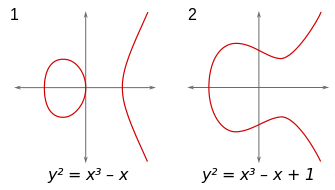
\includegraphics[width=225px]{images/ECC_1.png}
\end{center}
Sulla sinistra una curva a due componenti, sulla destra una curva ad una componente.
Si osservi le radici della cubica $x^3 + ax +b$, si hanno tre radici che possono essere:
\begin{itemize}
    \item 3 reali $\implies$ Curva a due componenti
    \item 1 reale e 2 complesse coniugate $\implies$ Curva ad una componente
\end{itemize}
 {{Si noti che le curve ellittiche sono sempre simmetriche rispetto all'asse delle $x$}}. Se non imponessimo radici distinte avremmo curve con cuspidi o con nodi, in queste particolari curve la tangente non è detto che esista unica (e questa cosa ci serve).

\subsection{Punto opposto $\mathbf{-P}$} La simmetria viene dal termine $y^2$, infatti:
$$ P = (x,y) \in E(a,b) \implies y^2 = x^3 + ax + b $$
definiamo dunque:
$$ -P = (x,-y) \implies (-y)^2 = y^2 = x^3 + ax + b $$
Dato $P=(x,y) \in E(a,b) $ si dice \emph{opposto} e si indica con $-P$ il punto $-P=(x,-y)$. Per il punto all'infinito si pone $0=-0$.

\subsection{Somma sulla curva ellittica}
Vogliamo definire un nuovo sistema a chiave pubblica, per fare ciò serve una funzione \emph{one-way trap-door}. Per avere una funzione per prima cosa dobbiamo definire un'operazione sull'insieme dei punti. Definiamo la \textit{somma} (attenzione, non ha nulla a che fare con la somma delle coordinate!
\paragraph{Cosa facciamo?} Facciamo l'intersezione tra la curva ellittica e una retta
\[
\begin{cases}
	y = mx + q \\
	y^2 = x^3 + ax + b
\end{cases}
\]
manipolando le equazioni mi trovo con una cubica della $x$. Le situazioni possibili sono:
\begin{itemize}
	\item un solo punto reale e due complessi coniugati;
	\item tre reali.
\end{itemize} 
Posso avere al massimo tre punti di intersezione.  Posso quindi prendere due punti sulla curva P e Q dato che ho due intersezioni esplicite ce ne sarà una terza per forza, chiamiamolo $R$. Il risultato di questa somma sarà $-R$ (per definizione).
\begin{center}
    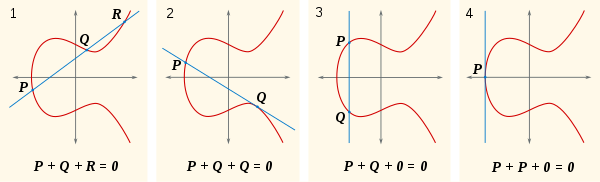
\includegraphics[width=390px]{images/ECC_2.png}
\end{center}

\subsubsection{Definizione di somma} Presi $P, Q, R \in E(a,b)$ se $P, Q, R$ sono disposti su una retta si pone:
$$ P + Q + R = 0 \implies P + Q = -R $$
\begin{center}
	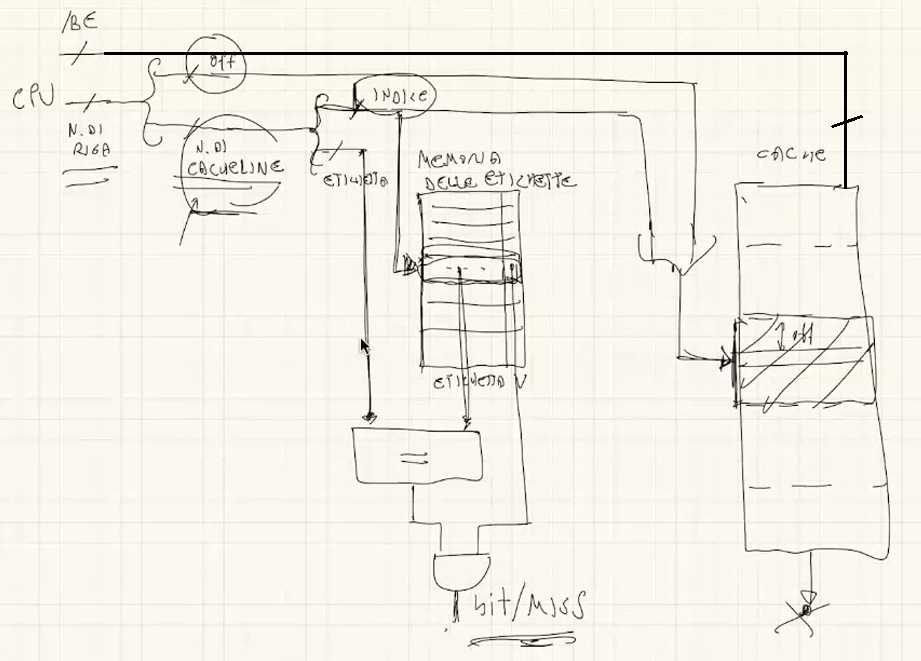
\includegraphics[scale=.8]{images/28.png}
\end{center}
Distinguiamo i vari casi:
\begin{itemize}
	\item $\mathbf{Q \neq \pm P}$. I punti $P, Q \in E(a,b)$. Trovo il terzo punto $R \in E(a,b)$ e utilizzo la formula della definizione. Nessun problema poichè $-R \in E(a,b)$
	\item Se $\mathbf{Q=-P}$ sommiamo il punto con il suo opposto
	$$P+(-P)=-0=0$$
	Si ricordi che nella nostra operazione l'elemento neutro è il punto all'infinito (si veda la terza figura prima della def.). 
	\item Se $\mathbf{Q = P}$ si considera la tangente alla curva nel punto $P$ (sempre definita per costruzione in quanto $4a^3+2tb^2 \neq 0$) e se ne vede l'intersezione con la curva. Si prende l'opposto del punto di intersezione tra tangente in $P$ e curva (può essere $O$).
	\begin{center}
		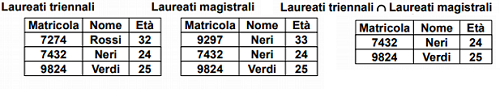
\includegraphics[scale=.85]{images/29.png}
	\end{center}
	Si noti che anche in questo caso se si fa passare una retta sull'estremo sinistro si ha una retta verticale e quindi la somma può dare il punto all'infinito (si veda la quarta figura prima della def.).
\end{itemize}

\subsubsection{Proprietà della somma}
\begin{itemize}
	\item \textbf{Chiusura}. $\forall P, Q \in E(a,b): P+Q \in E(a,b) $
	
	Dalla somma di due elementi otteniamo sempre un terzo elemento appartenente alla curva. 
	
	\item \textbf{Elemento neutro}. $ \forall P \in E(a,b): P + 0 = 0 + P = P $
	
	Per ogni punto appartenente alla curva ellittica esiste l'elemento neutro, ossia un punto che sommato al primo non lo altera.
	
	\textbf{NB}: Prendendo un punto $P$ e tracciando la retta all'infinito passante per $P$ l'altra intersezione è $-P$ quindi il risultato è $-(-P) = P$.
	
	\item \textbf{Inverso (opposto)}. $$ \forall P \in E(a,b)\,\, \exists! \, Q \in E(a,b) : P + Q = 0 = Q + P$$
	$$ Q = -P \implies P = (x,y), Q = (x, -y) $$ 
	
	Per ogni punto $P$ appartenente alla curva ellittica esiste uno e un solo punto $Q$ tale che $P+Q=0$
	
	\item \textbf{Commutativa}. $\forall P, Q \in E(a,b) P + Q = Q + P $
	
	\item \textbf{Associativa}. $ \forall P, Q, R \in E(a,b):\, (P + Q) + R = P + (Q + R) $
\end{itemize}

\subsubsection{Formulazione algebrica}
Dati \begin{align*}
	P = (x_P, y_P)&&Q = (x_Q, y_Q)&&S = (x_S, y_S) = P+Q
\end{align*}
abbiamo:
\begin{itemize}
    \item $\mathbf{Q \neq \pm P}$:
    \[
        \begin{cases}
        	\lambda = \frac{y_Q - y_P}{x_Q - x_P}\\
            x_S = \lambda^{2} - x_P - x_Q \\
            y_S = \lambda(x_P - x_S) -y_P 
        \end{cases}
    \]
    \item $\mathbf{P = Q}$:
    \[
        \begin{cases}
        	\lambda = \frac{3x_P^{2} + a}{2y_P}\\
            x_S = \lambda^{2} - x_P - x_Q \\
            y_S = \lambda(x_P - x_S)-y_P 
        \end{cases}
    \]
    
    NB: se $y_P = 0$ allora $P+P=0$
    \item $\mathbf{Q = -P}$: otteniamo il p.to all'infinito $$P+Q = 0$$
\end{itemize}

\section{Curve ellittiche su campi finiti}
In crittografia non possiamo usare le curve su campi reali: la crittografia ha bisogno di un'aritmetica veloce e assolutamente precisa (senza, ad esempio, errori di arrotondamento). Quello che facciamo è prendere curve definite su campi finiti (quindi un numero finito di elementi): vedremo le cosiddette \emph{curve prime}. 
\begin{itemize}
	\item Il campo è l'insieme $\mathbb{Z}_p=\{0,1,\dots,p-1\}$
	\item $p$ è numero primo
	\item La caratteristica di $\mathbb{Z}_p$ è $p$. 
	\item Imponiamo $p>3$ per poter utilizzare la forma normale di Weierstrass.
\end{itemize}
Non abbiamo più una figura continua, ma una nuvola di punti (cit.)! Noi consideriamo solo le curve prime per le quali $4a^3 + 27b^2 \text{ mod } p \neq 0$ (CNS per gruppo Abeliano).
\paragraph{Campo} Ridefiniamo quindi la curva:
$$ E_p(a,b) = \{ (x,y) \in Z_p^2 \mid y^2 \text{ mod } p = (x^3 + ax + b) \text{ mod } p \} \cup \{0\} $$
\begin{itemize}
	\item Si noti che essendo in modulo si lavora sempre nel primo quadrante: $x \geq 0, y \geq 0$.
	\item La curva sarà ancora simmetrica ma non rispetto a  $y = 0$, bensì rispetto $y = \lfloor \frac{p}{2} 	\rfloor$
	\item Inoltre tutti i valori saranno in $[0, p-1]$ per il modulo (elementi appartenenti a $\mathbb{Z}_p$).
	\pagebreak 
	\item Essendo simmetrica se $P=(x,y) \in E_p(a,b)$ allora
	$$-P = (x, p-y) \in E_p(a, b)$$
	Se $y^2 \equiv x^3 + ax + b$ allora $(p-y)^2 \equiv p^2 -2py + y^2 \equiv y^2$ poichè $p$ è lo zero nel campo.
\end{itemize}
Le formule della somma sono dunque le stesse ma si lavora in modulo (le divisioni diventano moltiplicazioni per l'inverso se non ci sono semplificazioni immediate, l'inverso c'è sempre perché lavoriamo modulo un numero primo). 
\begin{center}
	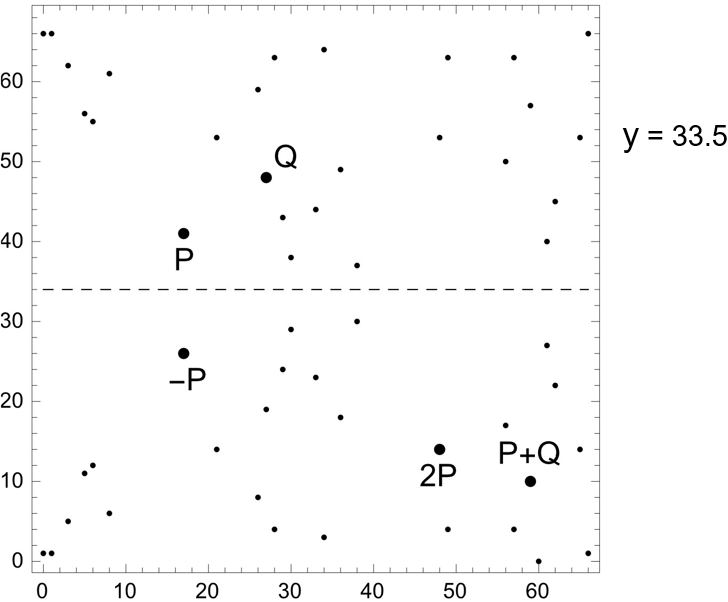
\includegraphics[scale=.5]{images/32.PNG}
\end{center}
\paragraph{Esempio} Prendiamo $P=(17,41) \in E_{67}(-1,1)$. L'elemento è rappresentato in figura. Calcoliamo l'opposto:
$$-P=(17,-41 \text{ mod }67)=(17, -41+67)=(17,26) \in E_{67}(-1,1)$$
La condizione per definire un gruppo Abeliano è valida: $(4a^3+27b^2) \text{ mod } p \neq 0$
\subsection{Formulazione algebrica}
Siamo nell'insieme $\mathbb{Z}_p$. Dati \begin{align*}
	P = (x_P, y_P)&&Q = (x_Q, y_Q)&&S = (x_S, y_S) = P+Q
\end{align*}
abbiamo:
\begin{itemize}
	\item $\mathbf{Q \neq \pm P}$:
	\[
	\begin{cases}
		\lambda = \frac{y_Q - y_P}{x_Q - x_P}\text{ mod } p\\
		x_S = (\lambda^{2} - x_P - x_Q)\text{ mod } p \\
		y_S = (\lambda(x_P - x_S) -y_P)\text{ mod } p 
	\end{cases}
	\]
	\item $\mathbf{P = Q}$:
	\[
	\begin{cases}
		\lambda = \frac{3x_P^{2} + a}{2y_P}\text{ mod } p\\
		x_S = (\lambda^{2} - x_P - x_Q)\text{ mod } p \\
		y_S = (\lambda(x_P - x_S)-y_P)\text{ mod } p 
	\end{cases}
	\]
\end{itemize}

\subsection{Ordine di una curva ellittica (cardinalità)}

\paragraph{Premessa} Cosa intendiamo con \emph{residuo quadratico}? Intendiamo un numero intero $q$ se esiste un intero $x$ tale che
$$x^2 \equiv q \text{ mod }p \longrightarrow x^2 \text{ mod } p = q$$

\paragraph{Definizione} L'ordine di una curva è il numero di punti che la curva possiede.
$$y^2=x^2+ax+b$$
Non esiste una formula precisa per trovare l'ordine: dipende dalla cubica. Prendo un valore $x\in \mathbb{Z}_p$
\begin{itemize}
	\item Si hanno al massimo $p$ valori per l'ascissa $x$, quindi mi aspetto circa $2p$ valori per l'ordinata $y$ (si ricordi che nella formula è posto il quadrato). Sommo $1$ per considerare il punto all'infinito:
	$$2p+1$$
	\item Non tutti i valori nel campo hanno una radice, quindi \textbf{\underline{sono molti meno}} di $2p + 1$.
	%\item In genere in $Z_p$ i residui quadratici che definiscono un punto sulla curva sono $\frac{p-1}{2}$.
	
	\item Il \textbf{teorema di {Hasse}} ci dice che se $N$ è l'ordine della curva prima $E_p(a,b)$ allora:
	$$ \mid N - (p+1) \mid \leq 2\sqrt{p}  $$
\end{itemize}
\paragraph{Esempio} Consideriamo la seguente curva
$$y^2\equiv (x^3+4x+4) \text{ mod }5$$
Calcoliamo i quadrati dei punti del campo, in modo da capire quali sono residui quadratici e quali no.
\begin{center}
	\begin{tabular}{c|c c c c c}
		\hline
		$y$ & 0&1&2&3&4  \\
		$y^2 \text{ mod }5$ & 0&1&4&4&1  \\
	\end{tabular}
\end{center}
Osserviamo che i numeri $0,1,4$ sono residui quadratici. Per la costruzione della curva consideriamo i possibili valori $x$.
\begin{align*}
	& \Longrightarrow y^2\equiv (x^3+4x+4) \text{ mod }5\\
	x=0 &\Longrightarrow y^2=4 \Longrightarrow (0,2), (0,3) \in E_5(4,4)\\
	x=1 &\Longrightarrow y^2=4 \Longrightarrow (1,2),(1,3) \in E_5(4,4)\\
	x=2 &\Longrightarrow y^2=0 \Longrightarrow (2,0) \in E_5(4,4)\\
	x=3 &\Longrightarrow y^2=3 \Longrightarrow \text{Non esistono punti di ascissa $3$}\\
	x=4 &\Longrightarrow y^2=4 \Longrightarrow (4,2),(4,3) \in E_5(4,4)
\end{align*}
Abbiamo $7$ punti, più il punto all'infinito: l'ordine è $8$.
\subsection{Costruzione di una funzione \emph{one-way trap-door}}
C'è una specie di parallelismo tra le operazioni in algebra modulare e le operazioni sulla curva ellittica:
\begin{itemize}
    \item la \textbf{moltiplicazione} (algebra modulare) diventa la \textbf{somma tra due punti} (curve ellittiche)
    \item l'\textbf{elevamento a potenza} $k$ (algebra modulare) diventa la \textbf{moltiplicazione di un punto per lo scalare} $k$ (curve ellittiche)
    \begin{align*}y^k=y \cdot y \cdot \dots \cdot y \Longrightarrow kP=P+P+\dots+P\end{align*}
\end{itemize}
La funzione deve essere one-way, quindi la moltiplicazione deve avere costo polinomiale. Non possiamo fare la somma $k$ volte: non è praticabile, abbiamo una complessità esponenziale rispetto alla dimensione di $k$ (algoritmo pseudopolinomiale, crescita lineare nel valore, crescita esponenziale nella dimensione). Per rendere il numero di operazioni proporzionale al logaritmo del valore ricorriamo a un'addattamento dell'algoritmo delle esponenziazioni veloce: \textbf{algoritmo dei raddoppi ripetuti}.

\subsubsection{Moltiplicazione scalare: algoritmo dei raddoppi ripetuti}
\paragraph{Operazione ed esempio} Calcolare $Q = kP$ è one-way. Dati i valori $k$ e $P$ è facile calcolare $Q$ (si fa in $O(\log k)$). Consideriamo un esempio:
\begin{align*}
	&Q=13P=(1+4+8)P\\
	&P \longrightarrow 2P \longrightarrow 2(2P)=4P \longrightarrow 2(4P)=8P
\end{align*}
Con 3 raddoppi calcoliamo $8P$. Concludiamo
$$Q=P+4P+8P=13P$$

\paragraph{Formalizzazione} 
\begin{enumerate}
	\item Dato $Q = kP$, riscrivo $k$ in notazione binaria: 
	\begin{align*}
		k = \sum_{i=0}^{t}k_i \cdot 2^i && k=(k_tk_{t-1}\dots k_2k_1k_0)
	\end{align*}
	Mi servono quindi il seguente numero di bit
	$$t+1 = \lfloor \log_2 k \rfloor + 1$$
	\item Si calcolano i vari raddoppi $$2P, 4P, \dots, 2^tP$$
	abbiamo $t$ raddoppi ciascuno come raddoppio del punto precedente.
	\item Si calcola $$Q = \sum_{i : k_i = 1} (2^iP)$$ in esattamente $t$ somme: $O(t) = O(\log_2 k)$ quindi lineare nella dimensione dell'input.
\end{enumerate}


\paragraph{Operazione inversa} Dati $P$ e $Q$, sulla curva $E_p(a,b)$, trovare il più piccolo $k$ tale che$$Q = kP$$
Non si conoscono algoritmi polinomiali (neanche  sub-exp) per risolvere il problema. Si parla di \emph{logaritmo discreto sulle curve ellittiche}.

\section{Protocollo Diffie-Hellman su curve ellittiche}
\paragraph{Premessa} Definiamo l'\emph{ordine di un punto} il più piccolo numero $n$ tale che
$$nB=0$$
\paragraph{Algoritmo}
\begin{itemize}
	\item Alice e Bob concordano una curva ellittica prima (che soddisfi la condizione di gruppo Abeliano) ed un punto $B$ della curva che abbia ordine molto grande. I punti e le curve sono già consigliate dal NIST, non si devono quindi creare da zero (come già visto nella versione dell'algebra modulare). Sono note e pubbliche.
	
	Il punto $B$ ottenuto è il generatore (ricordarsi cosa facevamo nella versione in algebra modulare: definizione di un intero primo e grande $p$ e di un generatore $g$).
	
	\item L'algoritmo prosegue così:
	\begin{enumerate}
		\item Alice genera un valore $n_A < n$ casuale, calcola $$P_A = n_AB$$ e lo invia in chiaro a Bob
		\item Bob riceve $P_A$. Genera un valore $n_B < n$ casuale, calcola $$P_B = n_BB$$ e lo invia in chiaro ad Alice
		\item Alice riceve $P_B$ e calcola $S = n_AP_B = n_An_BB$
		\item Bob riceve $P_A$ e calcola $S = n_BP_A = n_Bn_AB$
	\end{enumerate}
	ambo le parti hanno generato lo stesso $S$ e possono quindi generare la stessa chiave di sessione in vari modi (ad esempio $K = x_S \mod 256$).
\end{itemize}




\paragraph{Crittoanalista}
\begin{itemize}
	\item  Un crittoanalista non può fare nulla perché conosce $E_p(a,b), B, n, P_A, P_B$ ma non può trovare $n_A$ o $n_B$ se non risolvendo il problema del logaritmo discreto su curva ellittica.
	
	\item E' sempre possibile un attacco \emph{man-in-the-middle}: segue che la chiave va sempre estratta da un certificato!
	
	\item Il sistema col logaritmo discreto su curva ellittica è facile sulla macchina quantistica.
\end{itemize}


\section{Scambio di messaggi (equivalente di El-Gamal)}
\subsection{Algoritmo di Koblitz per la trasformazione del messaggio}
Per prima cosa bisogna preparare il messaggio in chiaro: deve essere trasformato in punto della curva ellittica. 
$$ m \xrightarrow{} P_m \in E_p(a,b) $$
\paragraph{Soluzione (sbagliata)}Si potrebbe pensare di usare $m$ come $x$ del punto ma potremmo incappare in una $y^2$ che non è un residuo quadratico, succede $\frac{1}{2}$ delle volte: una tecnica che ha successo solo metà delle volte non va bene!
\paragraph{Soluzione (giusta)} Si usa quindi \emph{l'algoritmo di Koblitz} che prende un intero $n$ e restituisce un punto sulla curva.
E' un algoritmo randomizzato. Si sceglie $h$ intero tale che $(m + 1) \cdot h < p$, eseguo quindi $i$ tentativi calcolando $x = m \cdot h + i$ con $0 \leq i < h$ e vedo se ottengo un punto valido:

\begin{verbatim}
// messaggio m, intero h, parametri della curva E
KOBLITZ(m, h, E):
    for(i=0; i < h; i++) {
        x = m*h + i
        z = (x^3 + E.a*x + E.b) mod E.p
        if z è un residuo quadratico {
            y = sqrt(z)
            return (x,y)
        }    
    }
    return "failure"
\end{verbatim}
\begin{itemize}
	\item La probabilità di fallimento è $\approx \left(\frac{1}{2}\right)^h$
	\item La probabilità di successo è circa $\approx 1 - \left(\frac{1}{2}\right)^h$
	\item Se ci è andata male si modifica il messaggio e si riprova.
\end{itemize}

\paragraph{Operazione inversa} A seguito della decifrazione otteniamo il punto della curva ellittica $(x,y)$, ma a noi interessa il messaggio $m$. Quindi:
$$ m = \left\lfloor \frac{x}{h} \right\rfloor = \left\lfloor \frac{mh+i}{h} \right\rfloor = \left\lfloor m + \frac{i}{h} \right\rfloor = m $$

\subsection{Cifratura e decifrazione}
Presi una curva $E_p(a,b)$ ed un suo punto $B$ con ordine elevato $n$, preso inoltre $h$ da usare per Koblitz ogni utente deve generare la sua coppia chiave pubblica-chiave privata.
\begin{itemize}
    \item \textbf{Chiave privata}. Bob estrae $n_{BOB} < n$
    \item \textbf{Chiave pubblica}. Calcola $P_{BOB} = n_{BOB} \cdot B$,
\end{itemize}

\paragraph{Alice} Alice vuole inviare un messaggio cifrato a Bob:
\begin{itemize}
    \item prende il messaggio $m$ e lo mappa ad un punto della curva $P_m \in E_p(a,b)$ con l'algoritmo di Koblitz
    \item sceglie un intero a caso $r$, calcola $$V = r \cdot B$$
    $V$ è un punto che \emph{protegge} $r$
    \item calcola $W = P_m + r \cdot P_{BOB}$
    \item invia la coppia $<V,W>$
\end{itemize}
Attenzione al parallelismo con El-Gamal: in entrambi i casi inviamo a Bob due elementi, di cui uno ha lo scopo di proteggere un valore e l'altro di mascherare il messaggio (che in questo caso rappresentiamo sottoforma di punto della curva)
\paragraph{Bob} Bob deve decifrare il messaggio ricevuto da Alice:
\begin{itemize}
    \item riceve la coppia $<V,W>$
    \item calcola (ricordando che $V=r\cdot B$ e $P_{BOB}=n_{BOB}\cdot B$):
        \begin{align*}
        	W -n_{BOB} \cdot V &= P_m + r \cdot P_{BOB} - n_{BOB} \cdot r \cdot B =\\
        	&= P_m + \cancel{r \cdot n_{BOB} \cdot B} - \cancel{r \cdot n_{BOB} \cdot B} = P_m
        \end{align*}  
    \item decifra la chiave con la formula detta assieme all'algoritmo di Koblitz.
\end{itemize}

\subsection{Sicurezza}
La sicurezza è legata al logaritmo discreto nelle curve ellittiche in quanto Eve può:
\begin{itemize}
    \item partendo da $V$ trovare $r$ e decifrare con:
    $$W - r\cdot P_{BOB} = P_m + \cancel{r \cdot P_{BOB}} - \cancel{r \cdot P_{BOB}} = P_m$$
    ma per trovare $r$ bisogna risolvere il problema del logaritmo discreto, cioè trovare uno scalare $r$ tale che $V = r \cdot B$
    
    \item partendo da $P_{BOB}$ può trovare $n_{BOB}$ e decifrare esattamente come fa Bob, ma anche qui c'è da risolvere $P_{BOB} = n_{BOB} \cdot B$
\end{itemize}
Si noti che inoltre $r$ è one-time quindi se si dovessere passare a brutare converrebbe comunque andare a ricavare la chiave privata.
\begin{itemize}
	\item Per attaccare RSA, DH, El Gamal (su algebra modulare) si hanno algoritmi di costo O($2^{\sqrt{b \log b}}$) con $b$ numero di bit del modulo. Questi attacchi sono basati sull' \emph{index calculus} in quanto si ha una struttura di campo.
	\item	Per attaccare protocolli su curve ellittiche invece si ha un costo O($2^{\frac{b}{2}}$) con $b$ bit dell'ordine di $B$, non essendo un campo ma un gruppo Abeliano si pensa che le tecnice usate per l'algebra modulare non verranno mai trasposte anche qui.
\end{itemize}
	\part{Applicazioni moderne della crittografia}

\chapter{Identificazione, autenticazione e firma digitale}

\section{Introduzione}
\paragraph{Identificazione} L' \emph{identificazione} prevede che un sistema isolato o in rete debba essere in grado di accertare l'identità di un utente che richiede di accedere ai suoi servizi.

\paragraph{Autenticazione} L' \emph{autenticazione} prevede che il destinatario di un messaggio possa essere in grado di accertare:
\begin{itemize}
    \item l'identità del mittente
    \item l'integrità del crittogramma ricevuto (che non sia stato modificato, che non sia stato sostituito)
\end{itemize}
\paragraph{Attenzione}\[\boxed{\text{Identificazione} \subset \text{Autenticazione}}\]
\paragraph{Firma digitale}
La \emph{firma digitale} ha le seguenti caratteristiche.
\begin{itemize}
    \item \textbf{{Non ripudiabilità}}. Il mittente non può negare di aver inviato il messaggio $m$.
    \item \textbf{{Autenticazione}}. Il destinatario deve essere in grado di autenticare il messaggio.
    \item Il destinatario non deve poter sostenere che $m' \neq m$ è il messaggio inviato dal mittente.
\end{itemize}
Tutto questo deve essere verificabile da terzi (per esempio un giudice)! Non sono modalità indipendenti, ciascuna estende le precedenti! Sono funzionalità utilizzate per contrastare gli attacchi attivi. Ci sono realizzazioni sia su cifrari simmetrici che asimmetrici, noi vedremo queste ultime versioni.

\subsection{Funzioni hash}
Una funzione hash: $f: X \xrightarrow{} Y$ è una funzione tale che:
$$ n = |X| >> m = |Y| $$
La cardinalità del dominio è molto più ampia della cardinalità del codominio. Essendo non iniettiva il codominio potrà essere partizionato in insiemi di elementi del dominio che condividono lo stesso valore hash (con la stessa \emph{collisione}).
$$ \exists\, X_1, X_2, \dots, X_m \subseteq X$$
Gli insiemi sono disgiunti, tali che: 
$$ X = X_1 \cup X_2 \cup \dots \cup  X_m $$
$$ \forall i, x : x \in X_i : f(x) = y $$
\begin{itemize}
	\item Si vuole che le dimensioni dei vari insiemi $X_i$ siano più omogenee possibile: quindi due elementi estratti a caso da $X$ hanno probabilità circa $\frac{1}{m}$ di avere la stessa immagine $y$.
	\item Si vuole che immagini \emph{simili} tra loro appartengano a sottoinsiemi diversi (quindi immagini hash diverse).
	\item Bisogna gestire le collisioni.
\end{itemize}
Non ci bastano queste proprietà in crittografia. 
\subsubsection{Funzioni hash \emph{one-way}}
Per le applicazioni crittografiche si devono avere le seguenti proprietà ($f: X \xrightarrow{} Y$):
\begin{itemize}
    \item $\forall x \in X$ è computazionalmente facile calcolare $$y = f(x)$$
    \item \textbf{Proprietà one-way}. 
    
    Per la maggior parte degli $y \in Y$ è computazionalmente difficile determinare $$x \in X: f(x) = y$$
    \item \textbf{Proprietà {claw-free}}. 
    
    E' computazionalmente difficile determinare $<x_1, x_2>$ in $X$ tale che: $$f(x_1)=f(x_2)$$
    cioè deve essere difficile individuare due elementi che hanno la stessa \emph{collisione}.
\end{itemize}

\subsubsection{MD5 (Message Digest, v5)}
\begin{itemize}
	\item Si tratta di una famiglia di algoritmi. 	Sono stati pubblicati MD2, MD4, MD5. Nei primi due furono trovate falle e Rivest propose MD5 nel 1992.
	
	\item Riceve in input un sequenza $S$ di 512 bit e produce un'immagine di 128 bit.
	
	Si \emph{digerisce} la sequenza riducendone la lunghezza ad $\frac{1}{4}$.
	
	\item Non resiste alle collisioni e nel 2004 è uscito di scena con debolezze varie. Si considera severamente compromesso (anche dallo stesso Rivest).
	
	Si usa ancora in altri contesti non crittografici.
\end{itemize}

\subsubsection{RIPEMD-160}
E' la versione matura del \emph{Message Digest} (MD*). Nata nel 1995 produce immagini di 160 bit e non presenta i difetti di MD5.

\subsubsection{SHA (Secure Hash Algorithm)}
\begin{itemize}
	\item Progettata dal NIST ed NSA nel 1993 (enti statunitensi).
	\item Opera su sequenze lunghe fino a $2^{64}$ bit e produce immagini di 160 bit.
	\item \textbf{E' crittograficamente sicura}.
	\begin{itemize}
		\item La prima versione: SHA-0 conteneva debolezze e fu quindi rivista portando allo SHA-1.
		
		\item Sono poi stati creati SHA-2: altri 4 algoritmi caratterizzati da digest più lunghi.
		
		\item Nel 2007 a causa dei problemi di MD5 e SHA-0 il NIST ha richiesto nuovi standard e nel 2012 è stato selezionato un algoritmo che è diventano SHA-3, pubblicato ufficialmente nel 2015.
	\end{itemize}
\end{itemize}

\paragraph{SHA-1 a titolo di esempio}
\begin{itemize}
	\item 
	Opera su sequenze fino a $2^{64}-1$ bit e produce immagini di 160 bit.
	E' largamente usata nei protocolli crittografici anche se non è più certificata come standard.
	
	\item Opera su blocchi di 160 bit contenuti in un buffer di 5 registri da 32 bit ciascuno in cui sono caricati inizialmente dei valori pubblici.
	Il messaggio $m$ viene poi concatenato con una sequenza di padding che ne rende la lunghezza multipla di 512 bit.
	
	\item Il contenuto dei registri varia nel corso dei cicli successivi in cui questi valori si combinano tra loro e con blocchi di 21 bit provenientei da $m$.
	Alla fine i registri contengono SHA-1($m$).
\end{itemize}
\begin{center}
	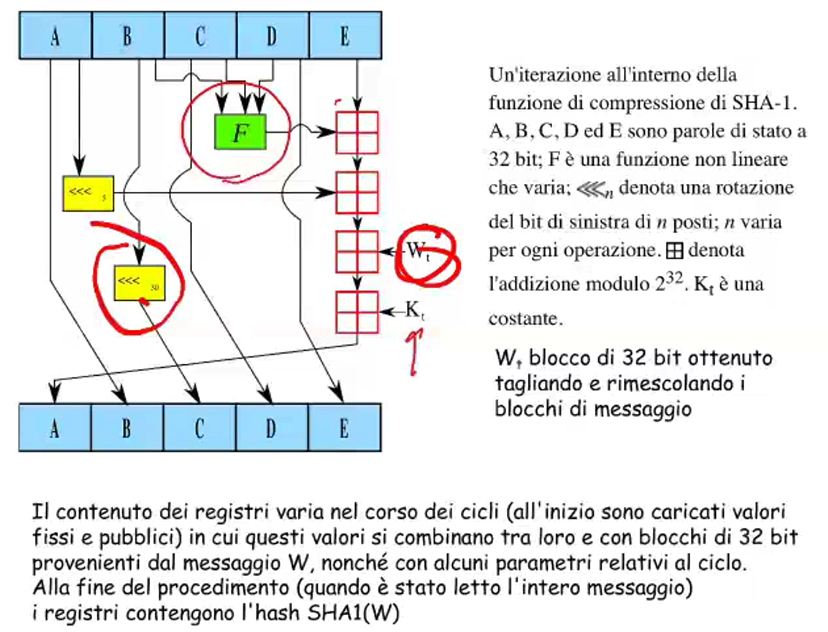
\includegraphics[scale=.65]{images/33.PNG}
\end{center}

\section{Protocollo di identificazione su canali sicuri}
Supponiamo di trovarci in un canale sicuro, cioè un canale protetto in lettura e scrittura, inaccessibile ad esterni indesiderati. Supponiamo di avere un utente che vuole accedere alle risorse su un calcolatore: per identificarsi utilizza \emph{username} e \emph{password}.
\paragraph{hash} Sono possibili attacchi da utenti interni, che potrebbero accedere al database e leggere le password. Per evitare problemi di questo tipo non si memorizzano mai le password in chiaro, ma un valore \emph{hash}.
\paragraph{Esempio UNIX} Quando un utente $U$ fornisce per la prima volta una password $P$ il sistema UNIX associa ad $U$ due sequenze binarie (\textbf{LE MEMORIZZA NEL FILE DELLE PASSWORD} al posto della password vera e propria, ricordare quanto visto a Sistemi Operativi):
\begin{itemize}
    \item $S$, un seme prodotto mediante generatore pseudocasuale;
    \item $Q = h(PS)$, hash della concatenazione di $P$ ed $S$.
\end{itemize}
Ad ogni successiva connessione il sistema:
\begin{itemize}
	\item prende l'hash $S$ dal file delle password e la password $P'$ \textbf{\underline{trasmessa}} dall'utente;
	\item li concatena ed applica la funzione hash.
\end{itemize} 
Se il risultato della funzione hash è uguale a $Q$ (posto sempre nel file delle password) allora avviene il riconoscimento.
\pagebreak
\begin{center}
	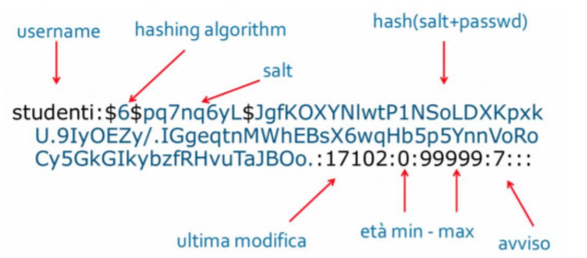
\includegraphics[scale=.85]{images/34.PNG}
\end{center}
\paragraph{Utilità} In questa maniera un accesso al file delle password non rivela informazioni importanti.

\section{Protocollo di identificazione su canali insicuri}
Se il canale è insicuro l'utente che vuole accedere la servizio non può trasmettere la password sul canale stesso: potrebbe essere intercettata durante la sua trasmissione in chiaro! Vediamo quindi un sistema di \emph{identificazione} basato su chiave pubblica e privata.

\paragraph{Sistema proposto} Per esempio siano $<e,n>$, $<d,n>$ le chiavi pubblica e privata di un utente $U$ (stessa struttura vista nell'RSA), che richiede l'accesso ai servizi offerti dal sistema $S$.
\begin{itemize}
    \item Il sistema $S$ genera un numero casuale $r < n$ e lo invia in chiaro a $U$
    \item L'utente $U$ calcola la \emph{firma di $U$ su $r$} \underline{utilizzando la chiave privata $d$}
    $$ f = r^d \text{ mod } n $$
    invia questo valore al sistema $S$
    \item Il sistema $S$ verifica la correttezza del valore ricevuto dall'utente $U$ calcolando:
    $$ f^e \text{ mod }  n =r$$
    Verifica l'uguaglianza. In caso di corrispondenza l'identificazione ha successo
\end{itemize}
\paragraph{Problema: sistemi non fidati} Se il sistema $S$ non è \emph{trusted} questo potrebbe inviare un $r$ particolare, anziché randomico, per cercare di carpire informazioni sulla chiave privata! La questione sarà affrontata col protocollo \emph{Zero Knowledge}.

\paragraph{Inversione rispetto all'RSA} Le operazioni di criptazione e decifrazione sono invertite (prima viene usata la chiave privata e poi la chiave pubblica) rispetto all'RSA. Ciò è possibile grazie alla seguente proprietà commutativa.
$$ (x^e \text{ mod } n)^d \text{ mod } n = (x^d \text{ mod } n)^e \text{ mod } n = x $$
Inoltre $f$ può essere generata solo dall'utente $U$ che possiede la chiave privata $<d,n>$. 

\section{Autenticazione su canale insicuro}
\subsection{Protocollo}
Per eseguire l'autenticazione invece si usa il MAC: \emph{message authentication code}.
\begin{itemize}
    \item Mittente e destinatario concordano una chiave segreta $k$
    \item Il mittente allega al messaggio un MAC:
    $$ A(m,k) $$
    allo scopo di garantire la provenienza e l'integrità del messaggio. Lo spedisce in coppia col messaggio in chiaro oppure col crittogramma
    \begin{align*}
    	<m, A(m,k)> && <C(m,k'),A(m,k)>
    \end{align*}
    \item Il destinatario entra in possesso di $m$, conosce il MAC $A(m,k)$ e ha già concordato la chiave $k$ col suo interlocutore (non è mai passata dal canale insicuro, quindi il crittoanalista non può conoscerla). Ricalcola $A(m,k)$ usando il messaggio $m$ ricevuto e ne confronta il valore col MAC inviato dal mittente. 
\end{itemize}
Se i MAC corrispondono allora l'autenticazione ha successo.

\subsection{\emph{Message Authentication Code} (MAC)}
Il \emph{Message Authentication Code} deve essere una immagine breve del messaggio, generabile solo se si consoce il valore $k$ (lo conoscono solo i due interlocutori). Ci sono varie implementazioni basate su cifrari asimmetrici, simmetrici e funzioni hash one-way. In particolare la versione one-way prevede:
$$ A(m,k) = h(mk) $$
con $h$ una \emph{funzione hash one-way}.

\paragraph{Sicurezza} E' sicuro in quanto $k$ viaggia nel MAC ed anche se venisse scoperto non è invertibile in maniera semplice.
Non può nemmeno sostituire tutto in quanto dovrebbe corredare il messaggio di un nuovo MAC che però non può calcolare essendo all' oscuro del valore di $k$.

\paragraph{Alternativa} Alternativa alle funzioni hash one-way, in un cifrario a blocchi in modalità CBC, è l'uso dell'ultimo blocco come MAC. La cosa è lecitissima in quanto la sequenza ottenuta rappresenta l'intero messaggio.

\section{Protocolli per la firma digitale}
\subsection{Caratteristiche della firma manuale e di quella digitale}
Riflettiamo sulle caratteristiche della firma manuale, da "traslare" nella firma digitale:
\begin{itemize}
    \item è autentica e non falsabile, prova che chi la ha prodotta è chi ha sottoscritto il documento;
    \item non è riutilizzabile, è legata al documento su cui è stata apposta;
    \item il documento non è alterabile, chi ha prodotto la firma è sicuro che questa si riferirà solo al documento sottoscritto nella sua forma originale;
    \item non può essere ripudiata da chi l'ha apposta costituendo prova legale di un accordo o dichiarazione.
\end{itemize}
Nella firma digitale si deve tenere conto delle cose già dette (autenticazione in primis) e di un altro dettaglio: essa non è la digitalizzazione della firma manuale, ma un qualcosa a se stante (essa non può essere la digitalizzazione di un documento originale firmato manualmente). Farla dipendere dalla firma manuale significa ridurne il potenziale. Ci sono protocolli che si basano sia su cifrari simmetrici che asimmetrici.

\subsection{Protocollo 1: messaggio in chiaro e firmato (DH)}
L'utente $U$ dispone di una $K_{upriv}$ e $K_{upub}$. $C$ e $D$ sono funzioni di cifratura e decifratura di un cifrario asimmetrico.
La firma funziona:
\begin{itemize}
    \item \textbf{Generazione della firma}.
    
    $U$ genera la firma decifrando il messaggio in chiaro
    $$f = D(m, k_{upriv})$$
    e spedisce all'utente $<U,m,f>$, dove $U$ è l'identificativo dell'utente
    \item \textbf{Verifica della firma}.
    
    L'utente riceve $<U,m,f>$, cifra il valore $f$ 
    $$C(f, K_{upub}) = m$$
    e verifica che il risultato sia proprio $m$
\end{itemize}
L'indicazione del mittente $U$ consente a $V$ di selezionare la $K_{upub}$ da utilizzare. Per far funzionare questo meccanismo è importante che $C$ e $D$ siano commutative, cioè
$$C(D(m))=D(C(m))=m$$

\paragraph{Requisiti della firma digiale} Questo protocollo soddisfa i requisiti della firma digitale. Si pensi a quali elementi influenzano la generazione della firma digitale: il messaggio $m$ e la chiave privata (quindi l'utente $U$, la chiave privata è nota solo a lui). 
\begin{itemize}
    \item E' autentica e non falsabile: $K_{upriv}$  è nota solo al mittente
    \item Il documento non può essere alterato in quanto $m$ e $f$ sarebbero inconsistenti
    \item $U$ non può ripudiare la firma perché \textbf{può averla prodotta solo lui}
    \item La firma non è riutilizzabile in quanto $f$ è immagine di $m$.
\end{itemize}

\subsection{Protocollo 2: messaggio cifrato e firmato}
Per trasmettere un crittogramma è necessario alterare il protocollo precedentemente introdotto: se cifriamo il crittogramma nella verifica della firma si restituisce il messaggio in chiaro, e la verifica della firma richiede la sola chiave pubblica. 
\paragraph{Firma e cifratura} Si distingua chiave di $U$ da chiave di $V$
\begin{itemize}
    \item $U$ genera la firma sempre a partire dal messaggio $m$ e dalla chiave privata sua:
    $$ f = D(m, K_{upriv}) $$
    \item Si calcola il crittogramma della firma appena generata con la chiave del destinatario.
    $$ c = C(f, K_{vpub}) $$
    \item Invia $<U, c>$, dove $U$ è l'identificativo dell'utente
\end{itemize}
\paragraph{Decifrazione e verifica} 
\begin{itemize}
	\item L'utente $V$ riceve la coppia $<U, c>$ e la decifra con la chiave privata sua:
	$$ D(c, K_{vpriv}) = f $$
	\item Verificando la firma (chiave pubblica del mittente) si ottiene anche il messaggio:
	$$ C(f, K_{upub}) = C(D(m, K_{upriv}), K_{upub}) = m $$
\end{itemize}
\subsubsection{Schema applicato all'RSA}
Per quanto riguarda le chiavi immaginiamoci il solito schema, sia per $U$ che per $V$. L'utente U, che vuole scrivere a $V$, fa i primi passi:
\begin{itemize}
    \item firma il messaggio $f = m^{d_u} \mod n_u$ (usa la chiave privata di $U$, cioè $<d_u,n_u>$);
    \item cifra il messaggio $c = f^{e_v} \mod n_v$ (usa la chiave pubblica di $V$, cioè $<e_v,n_v>$);
    \item spedisce la coppia ottenuta $<U, c>$;
\end{itemize}
L'utente V:
\begin{itemize}
    \item riceve e decifra $f = c^{d_v} \mod n_v$ (usa la chiave privata di $V$, cioè $<d_v,n_v>$);
    \item decifra $f$ con $k_{upub}$, $f^{e_u} \mod n_u = m$ (usa la chiave pubblica di $U$, cioè $<e_u,n_u>$).
\end{itemize}
Se $m$ è significativo concludo che è autentico.

\paragraph{Osservazioni} 
\begin{itemize}
	\item Per la correttezza del procedimento è necessario che $n_u \leq n_v$ affinché sia vero che $f < n_v$ e quindi $f$ possa essere cifrato correttamente.
	In questo modo tuttavia $V$ non può rispondere in quanto dovrebbero avere $n_u = n_v$ ma è poco sicuro e probabile.
	\item Possiamo ovviare quindi dando ad ogni utente due chiavi distinte: \begin{itemize}
		\item una per la firma $< H$ 
		\item una per la cifratura $> H$
	\end{itemize}  con $H$ pubblico e molto grande.
	NB: si può attaccare se ci si procura la firma di un utente su un messaggio apparentemente privo di senso
\end{itemize}


\subsubsection{Attacco con giochi algebrici}
Supponiamo che un utente $U$ abbia l'abitudine di inviare una risposta automatica (ack) al mittente ogni volta che riceve un messaggio $m$, e che questo messaggio sia il crittogramma della firma di $U$ su $m$.
\paragraph{Crittoanalista} Un crittoanalista attivo $X$ può decifrare i messaggi inviati a U:
\begin{itemize}
    \item $X$ intercetta $c$ firmato e crittografato inviato da $V$ a $U$, lo rimuove dal canale e lo rispedisce a $U$ con identificativo $X$. (cancella $<V,c>$ ed invia $<X,c>$)
    \item $U$ spedisce un ack ad $X$ in risposta
    \item $X$ usa l' ack per risalire al messaggio $m$ applicando le funzioni del cifrario con le chiavi pubbliche di $V$ e di $U$.
\end{itemize}
In particolare succede:
\begin{itemize}
    \item $V$ invia $c$ a $U$:
        $$
            \begin{cases}
                c = C(f, K_{upub}) \\
                f = D(m, K_{vpriv})
            \end{cases}
            \implies <V,c>
        $$
    \item $X$ intercetta la coppia, la rimuove dal canale prima che possa essere consegnata al destinatario, invia all'utente $U$ la coppia $<X,c>$
    \item $U$ riceve la coppia $<X,c>$ decifra $c$:
    $$ f = D(c, K_{upriv}) $$
    e verifica la firma con la chiave pubblica di X ottenendo:
    $$ m' = C(f, K_{xpub}) $$
    Il messaggio $m'$ ottenuto è privo di senso ($m' \neq m$) perchè la generazione della chiave non è avvenuta con la chiave di $X$, ma con quella di $V$. 
    \item Nonostante l'inconsistenza del messaggio l'utente $U$ l'ack $c'$ ad $X$:
    $$ f' = D(m', K_{upriv}) \Longrightarrow c' = C(f', K_{xpub}) $$
    \item \textbf{Giochini algebrici}.
    
    Il crittoanalista $X$ usa $c'$ ricevuto da $U$ per risalire ad $m$: decifra (con la chiave privata del crittoanalista) $$c': D(c', K_{xpriv}) = f'$$ e verifica (con la chiave pubblica del destinatario) $$f': C(f', K_{upub}) = m'$$Da $m'$ ricava (chiave privata del crittoanalista) $$f: D(m', K_{xpriv})=f$$verifica (chiave pubblica del vero mittente)$$f: C(f, K_{vpub}) = m$$
\end{itemize}
Attraverso questi giochini l'utente ha ottenuto $f$, e a quel punto tutto è in discesa: basta conoscere la chiave pubblica di $V$! Per evitare l'attacco si deve evitare l'ack automatico.

\subsection{Protocollo resistente agli attacchi}
Si evita di firmare il messaggio!
Si crea un hash del messaggio (SHA) con una funzione hash one-way e vi si appone la firma sopra.
La firma non è quindi più soggetta ai giochi algebrici appena visti.
\paragraph{Generazione della firma e cifratura}
\begin{itemize}
    \item il mittente $U$ calcola $h(m)$ e genera:
    $ f = D(h(m), K_{upriv})$
    \item calcola separatamente:
    $c = C(m, K_{vpub}) $
    \item spedisce a $V$ la tripla: $<U, c, f>$
\end{itemize}
\paragraph{Decifrazione e verifica}
\begin{itemize}
    \item $V$ riceve e verifica $<U, c, f>$
    \item decifra il crittogramma $c: m = D(c, K_{upriv})$
    \item calcola $h(m)$ (conosce la funzione \emph{hash} come il suo interlocutore) e $C(f, K_{upub})$ (conosce la chiave pubblica dell'interlocutore) e ne controlla l'uguaglianza, se sono uguali il messaggio è autentico
\end{itemize}
La firma si calcola più velocemente.

\subsection{Attacchi man-in-the-middle}
Le chiavi di cifratura sono pubbliche e non richiedono un incontro diretto per il loro scambio.
Un crittoanalista attivo può quindi intromettersi \textbf{\underline{nella fase iniziale}} comportandosi come $V$ agli occhi di $U$ e come $U$ agli occhi di $V$.
\begin{itemize}
    \item $U$ richiede a $V$ la sua chiave pubblica
    \item $X$ intercetta la risposta con $K_{vpub}$ e la sostituisce con la sua chiave pubblica $K_{xpub}$
    \item $X$ si pone in attesa dei crittogrammi spediti da $U$ a $V$ cifrati mediante $K_{xpub}$
    \item $X$ rimuove dal canale ciascuno dei crittogrammi, li decripta e li cifra con $K_{vpub}$ trafugata all'inizio, rispedendola a $V$
    \item $U$ e $V$ non si accorgono di nulla se il tutto è fatto velocemente
\end{itemize}
La cosa si risolve introducendo la \emph{Certification Authority}.

\section{Certification Authority - CA}
Sono infrastrutture/enti che garantiscono la validità delle chiavi pubbliche e ne regolano l'uso gestendo la distribuzione delle chiavi a chi vuole comunicare.
La CA autentica l'associazione emettendo un certificato digitale$$<\text{utente}, \text{chiave pubblica}>$$ 
Il certificato consiste della chiave pubblica e di una lista di informazioni relative al suo proprietario opportunamente firmate dalla CA. Mantiene quindi un archivio accessibile a tutti ma protetto da scritture non autorizzate. La chiave della CA è nota agli utenti che la mantengono protetta e la utilizzano per verificare la firma della stessa CA.

\subsection{Contenuto del certificato digitale}
Si compone principalmente di:
\begin{itemize}
    \item indicazione del formato (numero di versione)
    \item nome della CA che lo ha rilasciato
    \item numero seriale che lo individua univocamente nella CA emittente
    \pagebreak 
    \item specifica dell'algoritmo usato dalla CA per creare la firma digitale
    \item periodo di validità
    \item nome ed altre informazioni dell'utente a cui si riferisce il certificato
    \item nome dell'algoritmo, parametri e chiave pubblica usati dall'utente per cifr. e firm.
    \item firma della CA su tutto quanto
\end{itemize}
Quindi:
\begin{itemize}
	\item 
	Se $U$ vuole comunicare con $V$ può richiedere $K_{vpub}$ alla CA oppure direttamente a $V$ e poi lo convalida tramite la CA.
	
	\item Dato che $U$ conosce $K_{CA-pub}$ può controllarne l'autenticità e la validità.
	
	\item Ci si può mettere nel mezzo solo falsificando la certificazione ma si assume che la CA sia fidata.
	
	\item Esistono varie CA organizzate ad albero, la verifica quindi è più complicata in quanto si cerca il primo antenato comune tra le CA di $U$ e di $V$. Ogni utente poi mantiene in cache una copia dei certificati richiesti ed una copia di $K_{CA-pub}$ per non doverla richiedere.
\end{itemize}

\section{Protocollo finale con certificazione digitale}
\paragraph{Mittente} Il mittente $U$:
\begin{enumerate}
    \item si procura $cert$ di V (dove è presente la chiave con cui calcoliamo $c$)

    \item calcola $h(m)$ (con la sua chiave privata) e firma:
    $$ f = D(h(m),K_{upriv}) $$

    \item calcola $c$ (usando la chiave pubblica del destinatario, ottenuta dal certif. digitale):
    $$ c = C(m, K_{vpub}) $$

    \item spedisce la terna $<cert_U$, c, f$>$ ($cert_U$ contiene $K_{upub}$, quindi non è necessario trasmetterla separatamente)
\end{enumerate}
\paragraph{Destinatario} Il destinatario $V$:
\begin{itemize}
    \item riceve $<cert_U$, c, f$>$ e verifica l'autenticità di $cert_U$ (e di $K_{upub}$) tramite la CA.

    \item decifra il crittogramma:
    $$ m=D(c, K_{vpriv}) $$

    \item verifica l'autenticità della firma:
    $$ C(f, K_{upub}) = h(m) $$
\end{itemize}
\paragraph{Attenzione} La catena ha un punto debole: i certificati non più validi; è quindi cruciale controllare periodicamente con la CA i certificati scaduti.
	\chapter{Protocollo conoscenza zero (\emph{Zero Knowledge})}

\section{Idea Generale}
Un protoccolo \emph{zero knowledge} è un protocollo che permette ad un utente detto \emph{Prover} (il dimostratore) di dimostrare di avere una certa conoscenza ad un \emph{Verifier} (il verificatore) senza inviare alcuna informazione se non l'evidenza di avere questa conoscenza.

\paragraph{Esempio} Facciamo un esempio concreto: supponiamo che Peggy dica di poter sapere se il numero di granelli di sabbia di cui si compone una spiaggia è pari o dispari, e che Victor voglia controllare la veridicità di questa affermazione senza arrivare alla totale certezza ma avvicinandosi tramite una probabilità prossima ad 1. Supponiamo che Peggy risponda:
\begin{itemize}
    \item 1 se il numero è dispari
    \item 0 se il numero è pari
\end{itemize}
Immaginiamo il seguente algoritmo:
\begin{verbatim}
for i = 1 to k { // k numero di sfide che Peggy deve superare
    <P si volta>
    <V sceglie e in {0, 1} casualmente> // un po' come lanciare una moneta
    if (e == 0)
        <V rimuove un granello di sabbia>
    <V chiede a P il nuovo b[i]>
    if ((e == 0 && b[i] != b[i-1]) || (e == 1 && b[i] == b[i-1]))
        <vado alla prossima iterazione>
    else
        <P è un imbroglione -> STOP>
}
\end{verbatim}
Facciamo $k$ test per assicurarci che Peggy stia dicendo il vero. Se una sfida viene perduta allora Peggy è un imbroglione, e ci fermiamo: deve essere in grado di vincere tutte le sfide!
\paragraph{Probabilità} La probabilità, al passo k, che Peggy sia un impostore è pari a:
$$
    P(\text{Peggy è un impostore})=\frac{1}{2^k}
$$
altresì la probabilità che Peggy dica il vero è:
$$
    P(\text{Peggy dice il vero})=1 - \frac{1}{2^k}
$$
Se il Prover è onesto non ha problemi a rispondere a tutte le iterazioni in maniera corretta, se non lo è può solo provare ad indovinare, quindi la probabilità di vincere imbrogliando è pari a quella di \textbf{\underline{indovinare una sequenza di k bit casuali}}. Quanto detto, attenzione, non è una dimostrazione rigorosa.


\subsection{Proprietà generali}
Quali sono le proprietà che deve avere un protocollo per poter essere definito \emph{protocollo a conoscenza zero}?
\begin{itemize}
	\item \textbf{Completezza}. 
	
	Se ciò che dice P è vero e V è onesto allora V deve sempre accettare la dimostrazione.
	
	\item \textbf{Correttezza}.
	
	Se P dice il falso allora V può essere ingannato con probabilità $\leq \frac{1}{2^k}$, con $k$ scelto da V.
	
	\item \textbf{Conoscenza zero}.
	
	Se l'affermazione di P è vera V (anche se disonesto) non può acquisire alcuna informazione se non il fatto che P ha la conoscenza che dice di avere.
\end{itemize}

\section{Protocollo di identificazione Fiat-Shamir}
E' un protocollo di identificazione nel quale P dimostra a V la sua identità senza svelare altre informazioni. Si basa sulla difficoltà di invertire la funzione potenza nell'algebra modulare, ovvero di calcolare la raidce in modulo.
\paragraph{Precisamente} Abbiamo la formula 
$$t=s^2 \text{ mod } n$$
Dati $s,n$ ($n$ composto) è facile trovare $t$ (calcolare la potenza). Dati $t$ ed $n$ è difficile trovare $s$, cioè calcolare la radice in modulo.
$$s=\sqrt{t} \text{ mod }n$$
Il Verifier conosce $<t,n>$, il Prover deve convincere il Verifier di conoscere $s$. A situazione normale il Verifier riceve $s$ dal prover e calcola $t$ in tempo polinomiale: se il $t$ calcolato coincide col $t$ che già conosceva allora è sicuro che il Prover conosce $s$. Nel caso dello Zero Knowledge vogliamo dare al Prover una "quasi certezza" di questo senza che $s$ venga trasmesso sul canale. 

\subsection{Generazione della chiave da parte del Prover}
Il prover genera la chiave, sia quella pubblica che quella privata.
\begin{itemize}
    \item $P$ genera $p$ e $q$ numeri primi (grandi)
    \item $P$ calcola $n = p \cdot q$ (otteniamo un numero composto)
    \item $P$ sceglie $s$ numero casuale tale che $s < n$ ($s$ sarà il suo segreto)
    \item $P$ calcola $\boxed{t = s^2 \mod n}$
\end{itemize}
La chiave pubblica sono i valori conosciuti dal Verifier: $<t,n>$. La chiave privata è ciò che è conosciuto esclusivamente dal Prover: $<p, q, s>$. Nel protocollo il Verifier vuole assicurarsi che il Prover conosca la chiave privata senza accedere alla chiave privata.

\subsection{Autenticazione}
L'algoritmo di autenticazione prevede $k$ iterazioni con $k$ scelto da V. Dopo $k$ passi il V si convince che P conosce la radice (con la probabilità che abbiamo detto). Arriverà a questa conclusione senza entrare in contatto con i valori segreti. 
\begin{enumerate}
    \item P genera un intero $r < n$, calcola $$\boxed{u = r^2 \text{ mod } n}$$ e comunica $u$ a V
    \item V sceglie casualmente $e \in \{1, 0\}$ e lo comunica a P
    \item P calcola $z = r \cdot s^e \text{ mod } n$ e lo comunica a V
    \begin{itemize}
        \item $e = 0 \implies z = r \text{ mod } n = r$ (poichè $r<n$)
        \item $e = 1 \implies z = r \cdot s \text{ mod } n$
    \end{itemize}
    \item V calcola $x = z^2 \mod n$ e controlla se $x == (u \cdot t^e \text{ mod } n)$
    \begin{itemize}
        \item se sono uguali si passa alla prossima iterazione
        \item se sono diversi P è un impostore
    \end{itemize}
\end{enumerate}
Si noti che se tutto è corretto:
$$                                
x = z^2 = (r \cdot s^e)^2 \text{ mod } n= r^2 \cdot s^{2 \cdot e}  \text{ mod } n= u \cdot t^{e} \text{ mod } n
$$
Se facciamo calcoli distinti otteniamo:
\begin{align*}
	x&=z^2\text{ mod }n=r^2 \text{ mod }n=u &e&=0\\
	x&=z^2 \text{ mod }n=(r\cdot s)^2 \text{ mod }n=r^2 \cdot s^2 \text{ mod }n=u \cdot t \text{ mod } n&e&=1
\end{align*}

\subsection{Dimostrazione di completezza e correttezza}
\paragraph{Completezza} La completezza si ottiene con le ultime due formule poste nella pagina precedente! Se $P$ è onesto allora passa tutte le prove e $V$ accetta la dimostrazione.
\paragraph{Correttezza} Supponiamo che $P$ sia disonesto: non conosce $s$ e l'unica cosa che può fare è tentare di indovinare i valori di $e$ decisi da $V$.
\begin{itemize}
    \item \textbf{Se prevede $e = 1$}.
    
    Sceglie $r$ casualmente ma invia $u = \frac{r^2}{t} \mod n$, successivamente manderà\\ $z = r \mod n$. V andrà quindi a verificare: $x = z^2 = r^2$, $$u \cdot t = \frac{r^2}{t} \cdot t = r^2 \implies x = u \cdot t \text{ mod } n$$
    \item \textbf{Se prevede $e = 0$}.
    
    Esegue l'algoritmo corretto infatti $x = z^2 = r^2$, $$u \cdot t^e = u = r^2 \implies x = u \text{ mod } n$$
\end{itemize}
se prevede bene le formule ottenute sono quelle già calcolate. La probabilità con cui $P$ è in grado di prevedere il corretto valore di $e$ equivale a $\frac{1}{2^k}$, dove $k$ è il numero di iterazioni/challenge a cui viene sottoposto $P$ da $V$.

\subsection{Dimostrazione della proprietà Zero Knowledge}
\[\boxed{\text{Non abbiamo fatto la dimostrazione}}\]

\subsection{Sicurezza a confronto con altri protocolli}
Questo protocollo di autenticazione è un protoccollo sicuro da entrambi i lati, sia per chi si deve far riconoscere che per chi autentica le richieste. Pensiamo ad una generica autenticazione tramite crittografia asimmetrica:
\begin{itemize}
    \item il client si vuole autenticare presso un server
    \item il server dispone della chiave pubblica del client, chiede quindi al client di firmare un messagio $r$ casuale
    \item il client riceve $r$, lo firma e lo restituisce al server
    \item il server verifica la firma e se è corretta l'autenticazione è avvenuta
\end{itemize}
In questo scenario ci si deve fidare del server in quanto si prende un messaggio arbitrario e lo si firma con la propria chiave privata, questo tuttavia potrebbe essere problematico in quanto possono esistere degli input malevoli che permettono di ottenere informazioni circa la chiave privata del client. Un protocollo a zero knowledge invece pone entrambi i lati della comunicazione sullo stesso piano di diffidenza.

\clearpage
	\chapter{Protocollo SSL (\emph{Secure Socket Layer})}
\section{Introduzione}
\[\boxed{\text{L'utente $U$ desidera accedere via Internet a un servizio offerto dal sistema $S$.}}\]
SSL (\emph{Secure Socket Layer}) è alla base dei protocolli più diffusi nelle comunicazioni sicure. Lo portiamo come esempio perchè combina molte cose viste durante il corso. 
\begin{itemize}
	\item Oggi non si utilizza la versione che introdurremo, ma il TLS (\emph{Transport Layer Security}, variante con qualche modifica).
	\item Garantisce \textbf{confidenzialità} e \textbf{affidabilità} delle comunicazioni su internet proteggendole da intrusioni, modifiche e falsificazioni.
	\item Sviluppato inizialmente da \textit{Netscape} per mettere in sicurezza HTTP, è progettato in modo da permettere la comunicazione tra computer che non conoscono le reciproche funzionalità.
	\item Garantisce la confidenzialità tramite l'uso di un sistema ibrido: 
	\begin{itemize}
		\item cifrario asimmetrico per la costruzione e lo scambio delle chiavi di sessione;
		\item cifrario simmetrico per la cifratura delle comunicazioni.
	\end{itemize}
	\item Garantisce l'autenticazione dei messaggi accertando l'identità dei due partner attraverso sia un cifrario asimmetrico che tramite certificati digitali con un MAC (\emph{Message Autentication Code}, che usa una funzione hash one way crittograficamente sicuro).
	\item Si trova tra il TCP (trasporto) e HTTP (applicazione) ma è totalmente indipendente dal protocollo applicativo sovrastante (HTTPS = HTTP su SSL).
\end{itemize}

\section{Livelli in cui SSL è organizzato}
SSL è organizzato in:
\begin{itemize}
	\item \textbf{SSL record}.
	
	Livello più basso, connesso direttamente al protocollo di trasporto. Ha l'obiettivo di incapsulare i dati spediti dai livelli superiori assicurando confidenzialità ed integrità.
	
	\item \textbf{SSL handshake}.
	
	Instaura e mantiene i parametri poi usati da SSL record. Si permette a utente e sistema di:
	\begin{itemize}
		\item autenticarsi;
		\item negoziare gli algoritmi di cifratura e firma;
		\item stabilire le chiavi per i signoli algoritmi crittografici e per il MAC.
	\end{itemize}
	Il tutto permette di creare un canale di comunicazione sicuro, affidabile e autenticato tra utente e sistema, all'interno del quale SSL Record fa viaggiare i messaggi. Abbiamo uno scambio di messaggi preliminare (\emph{handshake}) per la creazione del canale sicuro: attraverso questi messaggi il sistema $S$ e l'utente $U$
	\begin{itemize}
		\item si identificano a vicenda, e
		\item cooperano nella costruzione delle chiavi segrete da impiegare nelle comunicazioni successive.
	\end{itemize}
\end{itemize}
Vediamo singolarmente le fasi.

\section{Fasi in SSL handshake}
\subsection{Messaggio \emph{client hello} inviato dall'utente $U$}
L'utente $U$ invia al sistema $S$ un messaggio con il quale:
\begin{itemize}
	\item si richiede la creazione di una connessione SSL;
	\item specifica i cifrari e meccanismi che supporta e le prestazioni di sicurezza richieste;
	\item invia una sequenza di byte casuali.
\end{itemize} 
Tutto questo è mandato in chiaro!

\paragraph{Esempio} Un esempio di \emph{client hello} è la \emph{cypher suite}. 
\[\boxed{\text{SSL\_RSA\_WITH\_AES\_CBC\_SHA1}}\]
Vuole utilizzare i seguenti cifrari:
\begin{itemize}
    \item \textbf{RSA} per lo scambio delle chiavi di sessione;
    \item \textbf{AES} come cifratura simmetrica;
    \item \textbf{CBC} come composizione dei blocchi;
    \item \textbf{SHA1} come funzione hash per il MAC.
\end{itemize}
Questo è un esempio di \emph{cipher suite}. Il sistema risponderà nella fase successiva: \emph{server hello}.

\subsection{Messaggio \emph{server hello} inviato dal server $S$}
Il sistema $S$ riceve il messaggio dell'utente $U$.
\begin{itemize}
	\item Seleziona una cipher suite che anche lui supporta (cerca di soddisfare le richieste dell'utente $U$)
	\item Invia un messaggio all'utente $U$ dove specifica la sua scelta.
	\item Appende dei byte casuali alla risposta. 
\end{itemize}
Anche questo è mandato in chiaro!

\paragraph{NB} Se $U$ non riceve il \emph{server hello} allora interromperà la comunicazione.

\subsection{Autenticazione (creazione certificato da parte del sistema $S$)}
Il sistema $S$ si autentica con $U$ inviandogli il proprio certificato digitale (e gli eventuali altri certificati fino al primo nodo comune nella catena delle CA).

\paragraph{NB} Se i servizi offerti da $S$ devono essere protetti negli accessi anche $S$ può richiedere a $U$ di autenticarsi inviando il suo certificato digitale. Avviene raramente in quanto la maggior parte degli utenti non ha un proprio certificato e in genere ci si accerta dell'identità di un utente in un secondo modo (autenticazione sul sito web ad esempio).

\subsection{Messaggio \emph{server hello done}}
Messaggio con il quale il server $S$ sancisce la fine degli accordi sulla cipher suite ed i parametri crittografici associati.

\subsection{Controllo del certificato da parte dell'utente $U$}
L'utente $U$ accerta l'autenticità del certificato ricevuto dal sistema $S$ tramite la data, tramite la CA che lo ha firmato, ecc. Estrae la chiave pubblica dal certificato. L'utente $U$:
\begin{itemize}
	\item costruisce il \emph{pre-master secret} costituito da una nuova sequenza casuale di byte;
	\item lo cifra con la chiave pubblica estratta dal certificato.
	\item spedisce il crittogramma al sistema $S$.
\end{itemize}


\subsection{Costruzione del \emph{master secret} presso l'utente $U$}
Sempre l'utente $U$ costruisce il \emph{master secret} partendo da:
\begin{itemize}
	\item il \emph{pre-master secret} (cifrato con RSA, si usa la chiave pubblica presente nel certificato di $S$);
	\item i byte casuali di \emph{client hello} e \emph{server hello} (\emph{client hello} lo ha di suo, mentre \emph{server hello} è stato inviato dal server).
\end{itemize} 
Applica a tutte queste sequenze delle funzioni hash one-way secondo una combinazione opportuna. Il nuovo valore ottenuto è il \emph{master secret}.

\subsection{Ricostruzione del \emph{master secret} presso il server $S$}
Anche il sistema $S$ si calcola localmente il master secret. Può farlo perchè possiede:
\begin{itemize}
	\item il \emph{pre-master secret}, appena ricevuto dall'utente $U$ e decriptato con la sua chiave privata
	\item i byte casuali di \emph{client hello} e \emph{server hello} (\emph{client hello} lo ha ricevuto dall'utente $U$, mentre \emph{server hello} lo ha di suo)
\end{itemize}
Entrambi gli utenti hanno il \emph{master secret}!

\subsubsection{Extra: Autenticazione dell'utente $U$ (se richiesto certificato a $U$)}
\begin{itemize}
	\item Se all'utente $U$ è richiesto un certificato ed egli non lo possiede il sistema $S$ interrompe l'esecuzione del protocollo.
	\item Altrimenti $U$ invia il proprio certificato allegando \emph{master secret} e la SSL-history (tutti i messaggi scambiati fino a quel momento) firmate con la sua chiave privata.
	\item Il sistema $S$ controlla certificato ed SSL-history: \textbf{nel caso in cui emergano ambiguità la comunicazione viene interrotta}.
\end{itemize}


\subsection{Messaggio \emph{finished} inviato sia dall'utente che dal server}
E' il primo messaggio protetto da \emph{master secret} e \emph{cipher suite} accordati. Il messaggio è costruito dall'utente $U$ e inviato al sistema $S$, poi costruito dal sistema $S$ ed inviato all'utente $U$. Il messaggio ha la stessa struttura ma cambiano i dati (la history).
\paragraph{Costruzione del messaggio} La costruzione avviene:
\begin{itemize}
    \item concatenazione di master secret, messaggi di handshake scambiati fino al momento attuale, e l'identità del mittente ($U$ o $S$);
    \item la stringa ottenuta viene trasformata applicando funzioni hash, sia con SHA-1 che con MD5. 
\end{itemize}
I due messaggi (quello trasmesso dall'utente $U$ e quello successivamente trasmesso dal server $S$) sono diversi in quanto il sistema $S$ aggiunge anche la \emph{finished} ricevuta da $U$ (che adesso fa parte della history). Non sono ovviamente invertibili perché costruiti tramite hash.
\paragraph{Uso del master secret} Il master secret viene usato per creare le chiavi:
\begin{itemize}
    \item chiave segreta per il cifrario simmetrico
    \item chiave per l'autenticazione del messaggio (MAC)
    \item \textit{initialization vector} per il CBC
\end{itemize}
Le terne di chiavi di $U$ ed $S$ sono diverse tra loro ma note ad entrambi, ciascuno usa la propria, quindi aumenta la sicurezza.

\section{SSL Record}
Successivamente i parametri vengono passati al SSL Record che si occupa del vero e proprio dialogo dei dati suddividendo i dati in blocchi, aggiungendo un MAC ad ogni blocco, cifrato con il protocollo simmetrico scelto e trasmesso al protocollo di trasporto sottostante. Il destinatario esegue il contrario.


\section{Sicurezza di SSL}
\begin{itemize}
	\item Nei passi di \textit{hello} i due partner creano e si inviano sequenze casuali per costruire la master secret, questo risulta in chiavi diverse ogni volta. Un crittoanalista non può riutilizzare i messaggi catturati sul canale per sostituirli a S successivamente.
	\item L'SSL record successivamente numera ogni blocco in maniera incrementale e lo autentica tramite MAC.
	Un blocco non può essere modificato in quanto il MAC è hash di:
	\begin{itemize}
		\item contenuto
		\item numero sequenziale del blocco
		\item chiave del MAC
		\item altre stringhe note e fissate a priori
	\end{itemize}
\item MAC e messaggio sono cifrati quindi prima di poterli alterare va forzato il cifrario.

\item Non si possono eseguire man-in-the-middle in quanto si usano i certificati.

\item Il pre-master secret è inviato cifrato con chiave pubblica quindi è sicuro.

\item Quindi solo $S$, proprietario della chiave privata associata al certificato può recuperare la pre-master key e quindi entrare in comunicazione con $U$.

\item Anche $U$ può essere autenticato se necessario.
Se è richiesto ma non avviene la comunicazione salta.
L'opzionalità di questa autenticazione ha reso usato questo protocollo in quanto può essere autenticato in altri modi, magari lato applicazione.

\item Le sequenze sono generate a partire da byte casuali quindi una sua predicibilità metterebbe a rischio tutto.

\item Il messaggio finished contiene tutta la history e quidi permette un ulteriore controllo finale. E' sicuro almeno quanto il cifrario più debole della cipher suite, ma non ci sono cifrari deboli lasciati dentro.
\end{itemize}






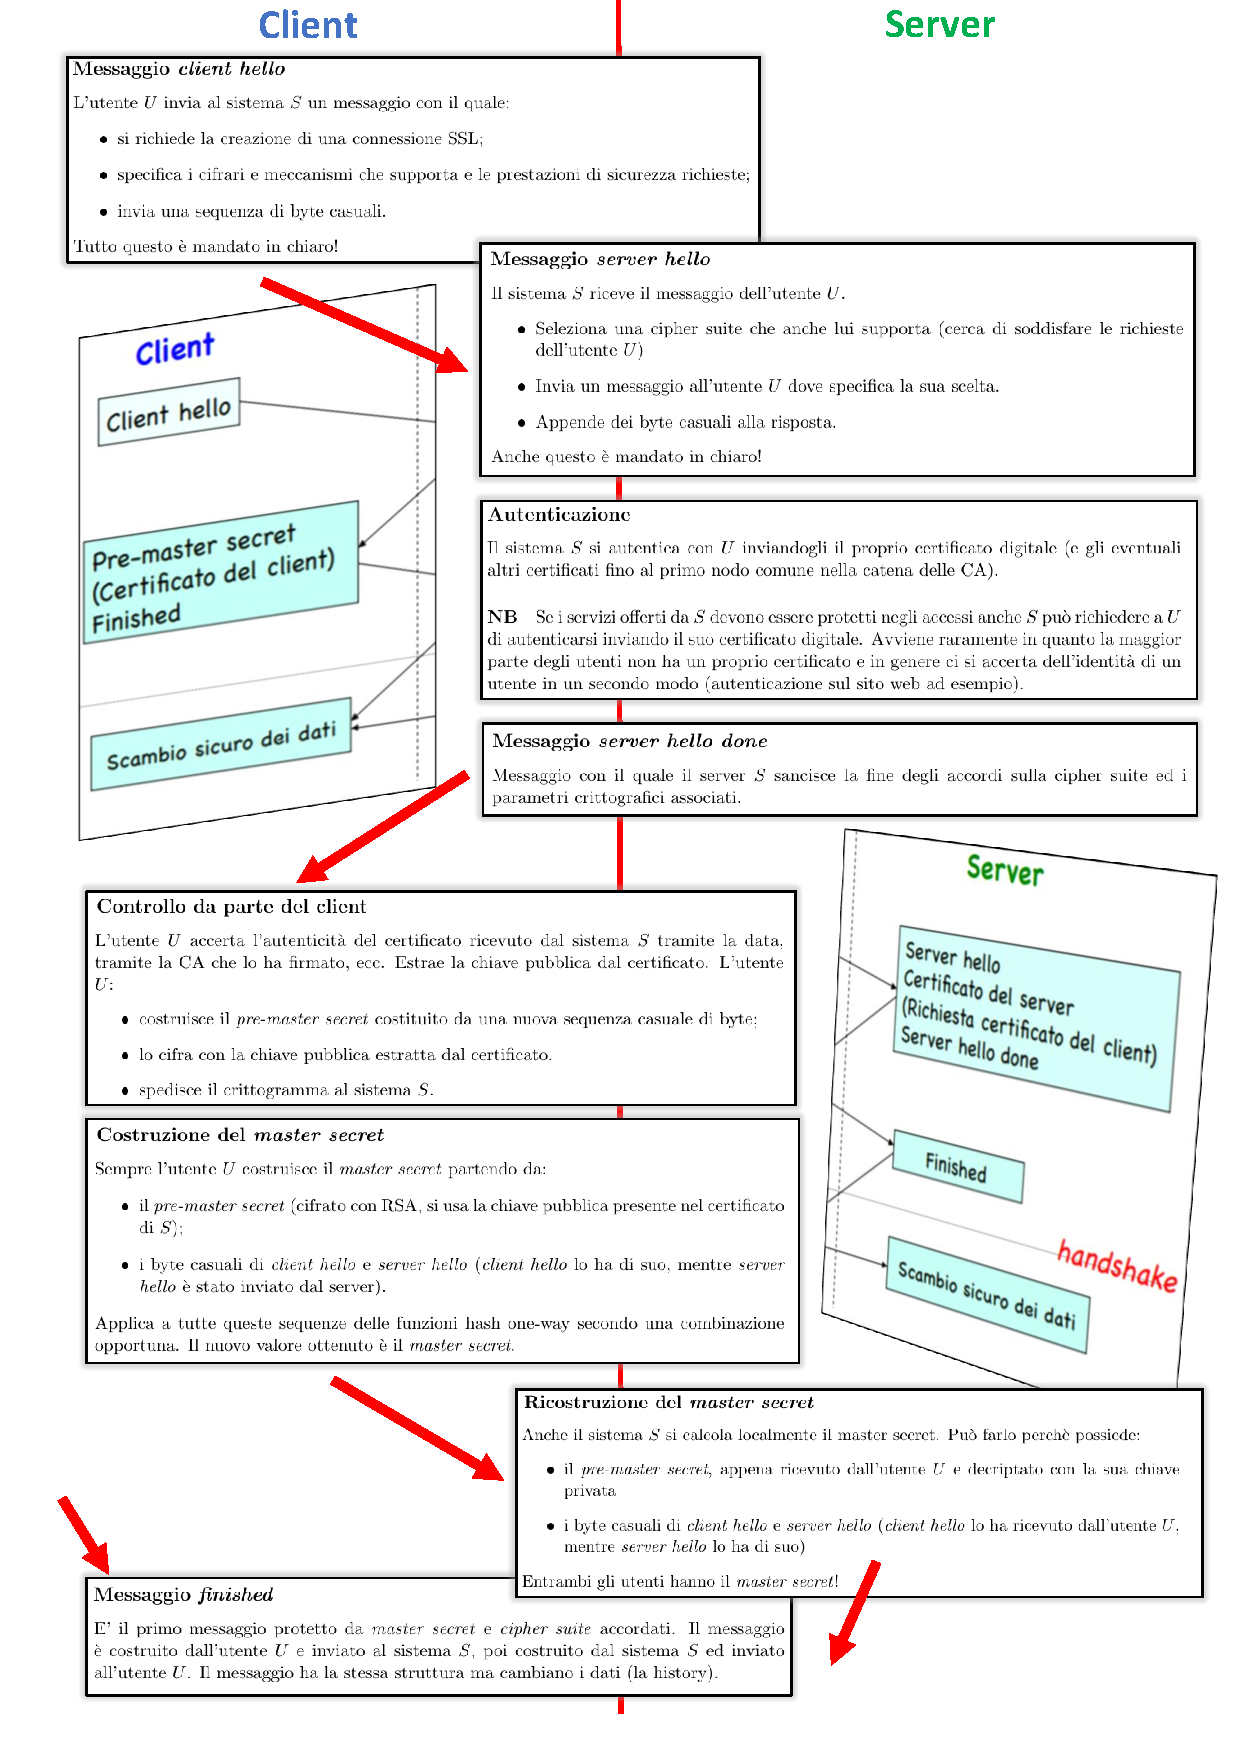
\includepdf[pagecommand={\thispagestyle{plain}},scale=0.84,pages=-]{pdf/schemassl}
	\chapter{Quantum Distribution Key (QDK)}
\section{Introduzione}
\begin{itemize}
	\item Il protocollo QDK è un protocollo alternativo a Diffie-Hellman per lo scambio delle chiavi.
	\item Permette di scambiare lunghe chiavi da utilizzarsi con one-time pad.
	\item Inoltre è già utilizzato in quanto non necessita dell'utilizzo di computer quantistici e se in futuro la tecnologia quantistica dovesse evolversi comunque questo protocollo sarebbe quantistico-resistente oltre che resistente al collasso della classe NP.
	
	Questo protocollo inoltre permette di accertare una eventuale intrusione, eventualmente si butta via la chiave, proprio per questo motivo non si può usare per scambiare messaggi.
\end{itemize}
\paragraph{NB} Esiste poi la crittografia post-quantistica che si occupa di cercare sistemi a chiave pubblica inattaccabili anche da macchine quantistiche. Ci si basa su problemi NP-completi che si sanno essere difficili anche con una eventuale supremazia quantistica.

\subsection{Principi della meccanica quantistica}
Sfruttiamo i seguenti principi della meccanica quantistica.
\begin{itemize}
    \item \textbf{Sovrapposizione degli stati}
    
    Un sistema quantistico si può trovare in più di uno stato allo stesso tempo. Matematicamente si intende una combinazione lineare dei possibili stati (i coefficienti sono numeri complessi). Il quadrato del modulo è la probabilità di individuare un particolare stato, quando effettuiamo una misurazione.
    
    \item \textbf{Decoerenza}.
    
    Quando si effettua una misurazione il sistema si \emph{perturba} quindi collassa solo in uno degli stati che prima erano sovrapposti. Si lascia quindi una traccia all'atto della misurazione, la usiamo per controllare circa eventuali intromissioni nella trasmissione
    
    \item \textbf{No-cloning}.
    
    Impossibilità di fare una copia di un sistema quantistico.
    Per copiare bisogna misurare, ma misurare significa modificare il sistema e quindi lasciare una traccia.
    \[\boxed{\text{No osservazione, no copia}}\]
    
    \item \textbf{Entanglement}.
    
    La possibilità che due sistemi creati con una correlazione tra loro continuino a mantenere la correlazione anche se portati a grandi distanze l'uno dall'altro (al contrario del principio di località della fisica classica). Quindi una misura eseguita su uno dei due influenza anche lo stato dell'altro seppur a larghissima distanza.
    
    \textbf{Esempio del fratello del prof. Luccio}: \emph{Il vostro partner va in Australia, se il vostro partner vi tradisce in quello stesso momento diventate cornuti (pur essendo a migliaia di chilometri di distanza)}.
\end{itemize}

\section{Protocollo BB84}
Nasce nel 1984 da Bennet e Brassard. Si fa tramite lo scambio di \emph{fotoni polarizzati} (particella elementare che costituisce la luce corpuscolare). Ogni fotone ha varie proprietà:
\begin{itemize}
	\item non ha massa;
	\item si muove alla velocità della luce;
	\item ha una sua \emph{polarizzazione} (piano di oscillazione del suo campo elettrico).
\end{itemize} 
Gli stati di polarizzazione da noi considerati sono quattro, che per comodità raggruppiamo in due \emph{basi di polarizzazione}.
\begin{center}
    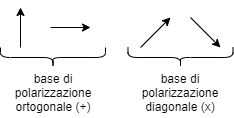
\includegraphics[width=150px]{images/QDK_1.png}
\end{center}
La direzione di polarizzazione può essere qualsiasi quindi scegliamo una base per rappresentarla (come se fosse un vettore).
In ognuno di questi stati codifichiamo un bit:
\begin{multicols}{2}
\begin{itemize}
    \item \textbf{verticale}: 0
    \item \textbf{orizzontale} : 1
    \item \textbf{+45°}: 0
    \item \textbf{-45°}: 1
\end{itemize}
\end{multicols}
\noindent Le scelte sono arbitrarie, stabilite dagli interlocutori: sanno quale base è stata adottata e compiono misurazioni secondo la base adottata. Se non si conosce quale base è stata usato non possiamo effettuare misurazioni corrette e certe ma solo probabilistiche: nel protocollo ci baseremo proprio su questa probabilità! La misura è completamente casuale perchè a seguito di una misurazione andiamo ad alterare il sistema, dunque perdiamo le informazioni precedenti.
\subsection{Premessa: struttura generale dell'hardware}
\begin{center}
    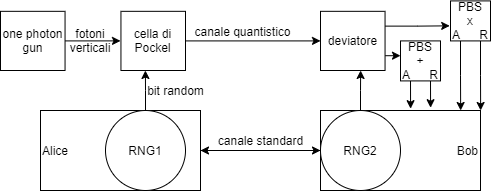
\includegraphics[width=300px]{images/QDK_2.png}
\end{center}
Ci si muove su due canali:
\begin{itemize}
	\item uno quantistico (fibra ottica), 
	\item uno standard (Alice e Bob devono comunicarsi le basi che hanno utilizzato per misurare, vedremo bene più avanti).
\end{itemize}
\paragraph{Lato Alice}  Supponiamo che Alice voglia trasmettere un messaggio a Bob.
\begin{itemize}
    \item \textbf{One Photon Gun}: emette singoli fotoni, tutti con polarizzazione verticale.
    \item \textbf{Cella di Pockel}: impone una certa polarizzazione. Questa è scelta da un \emph{Random Number Generator}, cioè Alice sceglie casualmente la polarizzazione del fotone.
\end{itemize}
\paragraph{Lato Bob} Bob riceve i fotoni, ma non sa cosa vuole trasmettere Alice. Non ha presente neanche la base: segue che per prima cosa dovrà scegliere come misurare il fotone, lo fa in modo casuale attraverso un \emph{Random Number Generator}.
\begin{itemize}
	\item \textbf{SW}: \textit{deviatore}, che si comporta in base al valore scelto da RNG2. In base al valore scelto cambia lo strumento con cui misuriamo il fotone.
    \item \textbf{PBS} (\emph{Beam splitter polarizzante}): ci da la corretta polarizzazione del fotone \textbf{se e solo se} la base di generazione e la base di misurazione sono le stesse utilizzate da Alice al momento dell'invio del fotone.
\end{itemize}
\subsubsection{\emph{Beam Splitter Polarizzante} (PBS)}
Il Beam Splitter polarizzante presenta un suo asse di polarizzazione $S$, in contrasto con la polarizzazione $F$ del fotone arrivato, mentre $\theta$ è l'angolo tra le due direzioni di polarizzazione. Misura il fotone tramite la deviazione verso una delle due uscite: 
\begin{itemize}
	\item A (assorbimento)
	\item R (riflessione)
\end{itemize}
La polarizzazione uscente non è quella del fotone in ingresso, ma una delle due polarizzazioni del PBS: $S$ o $S$ ortogonale. Da cosa dipende l'uscita? Dall'angolo $\theta$. Affermiamo che il fotone:
\begin{itemize}
    \item esce da A (polarizzazione $S$) con probabilità $\cos^2 \theta$
    \item esce da R (polarizzazione $S$ ortogonale) con probabilità $\sin^2 \theta$
\end{itemize}
\paragraph{Esempi in cui la polarizzazione è mantenuta} Può succedere che la polarizzazione uscente sia la stessa del fotone entrante. Sia $F$, ribadiamo, la polarizzazione del fotone entrante.
\begin{itemize}
    \item Se $\theta = 0$ abbiamo $F=S$, il fotone ha la stessa polarizzazione dello strumento. Le probabilità sono: 
    \begin{multicols}{2}
    \begin{itemize}
    	\item $\sin^2 \theta=0$ che esca da $R$;
    	\item $\cos^2\theta=1$ che esca da $A$.
    \end{itemize}
	\end{multicols}
	Il fotone uscirà sicuramente da $A$, con polarizzazione $S$.
    \item Se $\theta = 90$ allora $F \perp S$. Abbiamo come probabilità: 
    \begin{multicols}{2}
    \begin{itemize}
    	\item $\sin^2 \theta = 1$ che esca da $R$;
    	\item $\cos^2 \theta = 0$ che esca da $A$.
    \end{itemize}
\end{multicols} Il fotone uscirà sicuramente da $R$ e avrà come polarizzazione $S$ ortogonale. Anche in questo caso si conserva.
\end{itemize}
\paragraph{Distruzione dello stato precedente} Se $\theta = \pm45^{\circ}$ le basi di misurazione e di generazione sono diverse. Abbiamo come probabilità:
$$\cos^2\theta = \sin^2\theta = \frac{1}{2}$$
Il fotone ha pari probabilità di uscire da A o da R. La lettura attraverso il PBS potrebbe quindi distruggere lo stato quantistico precedente. Ricapitolando
\begin{center}
    \begin{tabular}{c|c|c|c|c}
        & 0 $\uparrow$ & 0 $\nearrow$ & 1 $\rightarrow$ & 1 $\searrow$ \\
        \hline
        + & $\uparrow$ & $\uparrow \rightarrow$ & $\rightarrow$ & $\uparrow \rightarrow$  \\
        x & $\nearrow \searrow$ & $\nearrow$ & $\nearrow \searrow$ & $\searrow$
    \end{tabular}
\end{center}
Le colonne indicano \textbf{bit e fotone inviato da Alice}, le righe \textbf{le basi di Bob}. Si ribadisce quanto già detto: se la base coincide si ottiene lo stesso stato, se la base non coincide allora lo stato precedente viene distrutto (i possibili stati sono equiprobabili). 
\subsection{Step del protocollo} 
Andiamo dunque al protocollo:
\begin{enumerate}
    \item Alice invia una sequenza $S_A$ sul canale quantistico.\\ Si segna le basi usate per generare i fotoni.
    \item Bob interpreta $S_A$ con le basi scelte casualmente.\\ Si segna quali basi ha usato per effettuare le misurazioni dei fotoni.
    \item Bob comunica ad Alice le sue basi \textbf{\underline{sul canale standard}}
    \item Alice risponde dicendo quali basi sono comuni alle sue.\\Dove le basi sono concordi si prendono i bit, dove le basi sono discordi si buttano.
\end{enumerate}
Si ha circa il 50\% di match. Alice e Bob, a seguito del confronto e in assenza di interferenze di Eve, possiedono $S_A' = S_B'$ sottosequenze identiche formate dai bit codificati dal mittente e decodificati dal destinatario con basi comuni:
$$ \mid S_A' \mid = \mid S_B' \mid = \frac{\mid S_A \mid}{2} $$
\paragraph{Variante al protocollo} Esiste un altro algoritmo quantistico di scambio di chiavi che si basa sull'entanglement: se i due estremi misurano con la stessa base fotoni correlati sono correlati anche i loro risultati quindi A e B misurano chiavi complementari.

\subsection{Esempio}
Consideriamo il seguente esempio, dove Alice trasmette una sequenza a Bob
\begin{center}
    \begin{tabular}{c|c c c c c c c c }
        $S_A$: & 1 & 0 & 1 & 1 & 1 & 0 & 0 & ...  \\
        Base adottata da alice: & + & x & + & x & x & + & x & ... \\
        Fotoni inviati da Alice: & $\rightarrow$ & $\nearrow$ & $\rightarrow$ & $\searrow$ & $\searrow$ & $\uparrow$ & $\nearrow$ & ...  \\
    
        & & & & & & & &  \\

        Base adottata da Bob: & + & x & + & + & + & x & x & ...  \\
        Lettura di Bob: & $\rightarrow$ & $\nearrow$ & $\rightarrow$ & $\uparrow$ 50\% & $\rightarrow$ 50\% & $\searrow$ 50\% & $\nearrow$ & ... \\
        $S_B$: & 1 & 0 & 1 & 0 & 1 & 1 & 0 & ...  \\
    \end{tabular}
\end{center}
Le basi concordi sono 1, 2, 3, 7 che portano alla sequenza:
$$ S_A' = S_B' = 1010 $$
Le riflessioni sarebbero già finite in assenza di crittoanalisti...

\subsection{Presenza del crittoanalista ed errori sperimentali}
La questione fondamentale è che la presenza del crittoanalista altera lo stato di polarizzazione dei fotoni (ricordare la proprietà della \emph{decoerenza}). 
\begin{itemize}
	\item Se c'è un crittoanalista esso si troverà nella stessa situazione di Bob, quindi deve scegliere le sue basi.
	\item Le basi scelte da Eve saranno indipendenti sia da quelle di Alice che da quelle di Bob. Se la base scelta da Bob coincide con quella di Alice allora non cambia nulla, se non coincide altera irreparabilmente il fotone!
	\item \textbf{Soluzione}. Alice e Bob fanno una verifica sacrificando un pezzo di $S_A'$ e $S_B'$:
	si scambia una porzione delle chiavi comuni in posizioni prestabilite comunicandole sul canale standard. A quel punto:
	\begin{itemize}
		\item se le due sequenze sono diverse la comunicazione viene interrotta;
		\item altrimenti usano la porzione rimanente come chiave o per costruire la chiave.
	\end{itemize}	
\end{itemize}
Riprendiamo l'esempio precedente e vediamo cosa succede con Eve nel mezzo:
\begin{center}
    \begin{tabular}{c|c c c c c c c c}
        $S_A$: & 1 & 0 & 1 & 1 & 1 & 0 & 0 & ... \\
        Base adottata da Alice: & + & x & + & x & x & + & x & ... \\
        Fotoni inviati da Alice: & $\rightarrow$ & $\nearrow$ & $\rightarrow$ & $\searrow$ & $\searrow$ & $\uparrow$ & $\nearrow$ & ... \\
    
        & & & & & & & & \\

        Base adottata da Eve: & + & + & + & x & + & x & + & ... \\
        Lettura di Eve: & $\rightarrow$ & $\rightarrow$ 50\% & $\rightarrow$ & $\searrow$ & $\uparrow$ 50\% & $\nearrow$ 50\% & $\rightarrow$ 50\% & ... \\
        $S_E$: & 1 & 1 & 1 & 1 & 0 & 0 & 1 & ... \\

        & & & & & & & & \\

        Base adottata da Bob: & + & x & + & + & + & x & x & ... \\
        Lettura di Bob: & $\rightarrow$ & $\searrow$ 50\% & $\rightarrow$ & $\uparrow$ 50\% & $\uparrow$ & $\nearrow$ & $\searrow$ 50\% & ... \\
        $S_B$: & 1 & 1 & 1 & 0 & 0 & 0 & 1 & ... \\
    \end{tabular}
\end{center}
\noindent Prendiamo i valori con basi concorde:
$$ S_A' = 1010 \neq  1111 =S_B' $$
\begin{itemize}
	\item Supponiamo quindi che si sacrifichi il secondo bit: $0 \neq 1$ e quindi ci si accorge di una intrusione.
	\item I bit non perturbati sono quelli per cui le 3 basi coincidono: $\frac{1}{4}$ delle volte. Quindi se Eve interviene: circa la metà di $S_A'/S_B'$ sarà differente.
	\item La verifica dell'intrusione è quindi importantissima, permette di sapere di eventuali intrusioni e quindi evitare di perdere informazioni.
\end{itemize}
Si osservi che le variazioni nello stato di polarizzazione non dipendono solo dall'intrusione di Eve: possiamo avere errori generici in fase di trasmissione dei fotoni, delle letture, ecc...
\begin{itemize} 
	\item Si stabilisce un \textbf{\emph{quantum bit error rate}} (QBER): una percentuale prevedibile di bit errati (dovuti a errori dell'apparato sperimentale).
	\item Si confrontano $S_A'$ e $S_B'$:
	\begin{itemize}
		\item se il numero di errore è $>$ QBER allora c'è stata una intromissione (e interrompiamo la comunicazione);
		\item altrimenti sono solo errori sperimentali e si correggono tramite correttori di errori.
	\end{itemize}	
	\item Eve potrebbe intercettare pochi fotoni e quindi farsi passare per errori dell'apparato pur conoscendo alcuni bit della chiave. Proprio per questo motivo anziché usare la sequenza scambiata si usa farne l'hash ed usare quello come chiave, in questo modo se cambiano anche solo pochi bit l'hash cambia enormemente.
	
	\item Le comunicazioni su canale standard possono anche essere in chiaro, è bene tuttavia che siano autenticate, magari tramite MAC (simmetrico con chiave scambiata in anticipo).
\end{itemize}

	\chapter{Bitcoin}
\section{Introduzione}
Il Bitcoin non è propriamente una moneta, ma un sistema di pagamento. Sfrutta i protocolli crittografici per due aspetti:
\begin{itemize}
	\item generare nuova moneta
	\item attestare il possesso della valuta da parte degli utenti.
\end{itemize} 
Nel compiere una transazione è necessario indicare una chiave privata: è l'unica cosa che permette di accertare il possesso dei Bitcoin, perdere la chiave significa perdere i Bitcoin. 
\paragraph{Nascita} Nasce nel 2008 con la pubblicazione di \emph{Bitcoin: a peer to peer Electronic cash system} a cura di \emph{Satoshi Nakamoto} (pseudonimo per una persona o un gruppo ancora ignoto).
\begin{itemize}
	\item Nel 2009 viene rilasciato il primo software per partecipare (bitcoin-core) ed il 3 Gennaio 2009 viene creato il \emph{blocco genesi}. 
	\item Il 12 Gennaio 2009 avviene la prima transazione: Satoshi Nakamoto invia 10 Bitcoin ad Hal Finney (il creatore del proof of work).
	\item Nel 2010 avviene la prima transazione commerciale: vengono pagate due pizze.
\end{itemize}

\paragraph{Caratteristiche} 
\begin{itemize}
	\item Questo sistema distribuito è caratterizzato da un libro contabile (\emph{ledger}) pubblico e distribuito costituito da singoli blocchi concatenati tra di loro: la \emph{blockchain}.
	\item La \textbf{blockchain} è una lista di blocchi contenenti centinaia di transazioni: si parla di catena perchè ogni blocco è legato ai precedenti tramite il calcolo di una funzione hash. 
	\item \textbf{Il primo blocco}. Il blocco genesi è il primo blocco di questa catena: con questo si sono creati i primi 50 bitcoin.
	\item \textbf{Numero di bitcoin generati con la creazione di un nuovo blocco}.
	
	Ogni volta che si riesce ad aggiungere un nuovo blocco si creano nuovi bitcoin ed ogni 4 anni circa si dimezza la moneta generata (inizialmente 50 bitcoin per blocco, ora 6.25 per blocco).
	\item \textbf{Deadline per la creazione di Bitcoin}. 
	
	La generazione ha un tempo massimo infatti nel 2140 l'aggiunta di blocchi non genererà più nuova moneta.
\end{itemize}

\section{Funzionamento}
Dopo aver scaricato il software necessario l'utente genera una sua coppia di chiavi
$$<K_A[\text{pub}], K_A[\text{priv}]>$$
\begin{itemize}
    \item \textbf{Chiave pubblica} $K_A[\text{pub}]$: costituisce l'indirizzo identificativo dell'utente, si usa per ricevere Bitcoin e \textbf{\underline{per verificare la firma}}
    \item \textbf{Chiave privata} $K_A[\text{priv}]$: si usa per firmare le transazioni (quindi per spendere)
\end{itemize}
Il tutto si basa sulla \textbf{crittografia a curve ellittiche}. 

\paragraph{Attenzione} Nel caso in cui venga persa la chiave privata non potremo più porci come legittimi proprietari del Bitcoin. Chiunque individui la chiave privata può porsi in modo legittimo come proprietario.

\paragraph{Wallet} Il \emph{wallet} è l' insieme delle credenziali che attestano la proprietà dei BTC: la coppia indirizzo/chiave privata. Ogni utente, nel software di gestione, ha un suo Wallet.

\subsection{Transazione}
La transizione è lo scambio di valuta tra due utenti. Immaginiamo che Alice voglia inviare un numero di $x$ BTC a Bob, il messaggio avrà la forma $m$ e verrà corredato da \emph{hash} e \emph{firma}
\begin{align*}
	m &= {\text{address}}_A - x - {\text{address}}_B\\
	h &= SHA_{256}(m)\\
	f &= D(h, K_A[priv])
\end{align*}
Nel compiere la transizione verrà diffusa in rete (rete peer-to-peer, comunicazione di tipo broadcast) la coppia $<m, f>$\footnote{Attenzione al refuso sul libro, si trasmette $f$ e non $h$.}.
\paragraph{Attesa} Essendo su un sistema distribuito il destinatario deve aspettare che la rete convalidi la transazione e richiede almeno 10 minuti.
\paragraph{Molteplicità dei rami di blockchain} Dopo 10 minuti il blocco verrà aggiunto alla blockchain, bisogna poi aspettare l'aggiunta di altri 6 blocchi al nostro ramo per essere sicuri al 100\% di aver compiuto una transazione: questo perchè sulla catena di blockchain si formano vari rami. Il ramo delle transazioni considerate effettivamente valide è solo quello ufficiale: chi compie transazioni deve stare attento su questo, altrimenti le transazioni potrebbero non essere valide (in quel caso ci si trova su \emph{blocchi orfani}, chi ha pagato è come se non avesse pagato).

\section{Frazionamento delle transazioni} Il frazionamento delle transazioni è questione macchinosa.
\begin{center}
	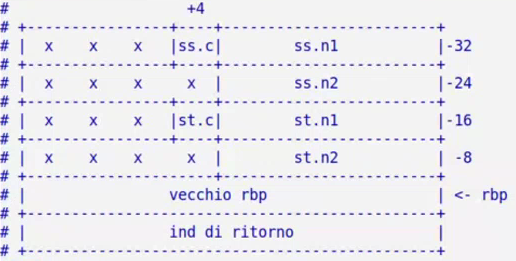
\includegraphics[width=320px]{images/31.png}
\end{center}
\subsection{Primo esempio con Bob}
Supponiamo di avere Bob che ha ricevuto 50 Bitcoin da un investitore: questi bitcoin sono l'input. Bob vuole spendere queste "monete", ma l'unica cosa che vuole fare inizialmente è trasmettere 0.5 Bitcoin ad Alice. 
\paragraph{Problema} Il patrimonio in mano a Bob è rappresentato da una o più transazioni, non è possibile scindere il contenuto di una transazione trasmettendo soltanto 0.5 Bitcoin e ignorando i rimanenti 49.5 Bitcoin. Se supponiamo i 50 Bitcoin come una banconota è come se Bob tagliasse con le forbici un pezzo di banconota. 
\paragraph{Soluzione} Nella transazione dobbiamo trasmettere tutti e 50 i Bitcoin, divideremo la cosa nel seguente modo:
\begin{itemize}
	\item 0.5 Bitcoin vanno ad Alice
	\item 49.5 vengono trasferiti a un indirizzo in mano a Bob (in un certo senso indica di volerli spedire a se stesso, potrebbe indicare la sua stessa chiave pubblica ma di solito non si fa così\footnote{Per mantenere l'anonimato}).
\end{itemize}
\subsection{Secondo esempio con Alice}
Successivamente Alice può spendere o meno i bitcoin ricevuti. Supponiamo che voglia trasmettere a un impiegato 0.8 Bitcoin. Può farlo unendo nell'input l'output di più transazione, precisamente:
\begin{itemize}
	\item 0.5 Bitcoin ricevuti prima da Bob
	\item 0.1 Bitcoin ricevuti da uno sconosciuto (ah quindi Alice parla con gli sconosciuti)
	\item 0.2 Bitcoin dalla sorella
\end{itemize}
Si possono spendere \textbf{output non spesi di precedenti transazioni} a noi destinate.

%La somma degli input deve sempre essere maggiore o uguale alla somma degli output, se è uguale pagamenti normali, se è maggiore quelli in più vengono aggiunti al primo che convalida il blocco (perché può aggiungere questo movimento).
%Per incentivare questa conferma si usa quindi lasciare questa \emph{fee} al miner.

\subsection{Validazione}
Gli utenti ricevono dal broadcast queste transazioni, le controllano (cercano nel passato se la valuta è presente nel conto di chi invia) le mettono assieme a gruppi (100, 200 anche 1000) e poi provano ad aggiungerle alla blockchain.

\paragraph{Come avviene l'aggiunta?} Ci sono vari modi per aggiungere i blocchi alla blockchain, noi vedremo il \emph{proof of work}.

\paragraph{\emph{double spending}} La blockchain previene il \emph{double spending}: per fare un paragone con la realtà è come se io pagassi due servizi diversi usando la stessa moneta, solo che al pagamento del secondo servizio i soldi non dovrebbero esserci più (sono già stati usati!). La cosa succede con la creazione di nuove transazioni nel periodo di validazione. 

\section{Struttura di un blocco della \emph{blockchain}}
Sono un nodo: arrivano le transazioni, le raggruppo in blocchi e cerco di validarle. 
\begin{center}
    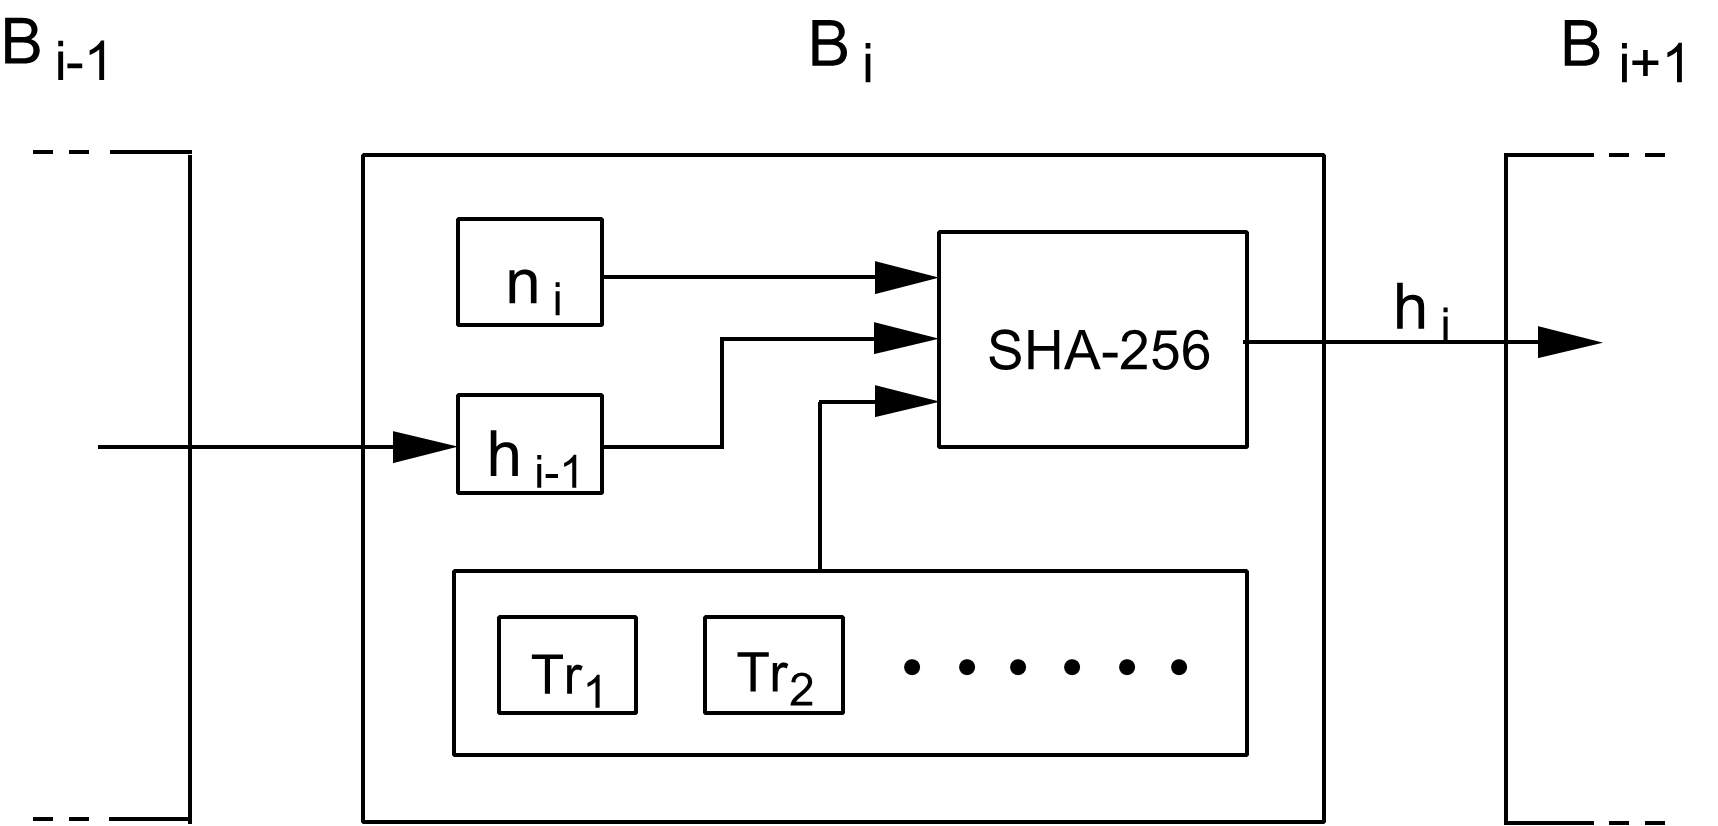
\includegraphics[width=220px]{images/Bitcoin_1.png}
\end{center}
\begin{itemize}
	\item Creo un blocco che le contiene, aggiungo la transazione finale che redirige verso di me destinatario la ricompensa.
	\item Nel blocco c'è $h_{i-1}$ cioè l'hash del blocco precedente nella catena: è importante perchè stabilisce la concatenazione col blocco precedente 
	\item Nel blocco c'è $n_i$ detto \emph{nonce}, un intero.
\end{itemize} 
Di queste informazioni faccio l'hash SHA-256 ed ottengo $h_i$, che andrà in ingresso nel blocco successivo. 
\paragraph{Richiesta} 
\begin{itemize}
	\item La richiesta è quella di ottenere un $h_i < $ di una certa soglia fissata dal sistema.
	\item Come faccio? Con una ricerca enumerativa: trovare quel valore intero $n_i$ (il \textit{nonce}) tale da soddisfare la richiesta. La richiesta è soddisfatta se troviamo un $h_i$ con $T$ zeri all'inizio.
	\item Il parametro $T$ è fissato dal sistema e varia in base alla potenza della rete.
	Questo è scelto in modo da portare il tempo di validazione di un blocco a circa 10 minuti.
	In media ci vogliono $2^T$ tentativi.
\end{itemize} 
\section{Miner e mining} Chi cerca di attaccare un nuovo blocco individuando il \textit{nonce} è detto \textbf{miner}. I miner sono i nodi che validano le transazioni aggiungendo nuovi blocchi alla blockchain. Si parla di \textbf{validazione tramite mining}.
\[\boxed{\text{La \emph{proof of work} è la ricerca del \textit{nonce}.}}\]
\begin{itemize}
	\item Cercare il \textit{nonce} è difficile
	\item Verificare il \emph{nonce} è semplice, quindi chi lo trova lo diffonde in broadcast a tutti i nodi, gli altri lo verificano, controllano la validità delle transazioni ed esprimono il loro consenso: prendono il nuovo nodo e cercheranno di attaccare nuovi nodi ad esso.
	\item Se la rete ad un certo punto ha delle biforcazioni si tende a privilegiare i rami con più transazioni perché è più probabile che siano accettati da tutta la rete.
\end{itemize}

\paragraph{Mining pool} Inizialmente Bitcoin doveva essere democratico e quindi tutti avrebbero potuto partecipare al mining, quello che è successo invece è stato che alcuni piccoli gruppi di utenti hanno unito le forze e messo a disposizione grande hardware per minare tutti assieme, ci si spartisce quindi lo spazio di ricerca del nonce e si dividono i profitti tra i vari partecipanti.

\paragraph{Aspetti sociali} Il mining ormai è poco sociale in quanto lo fanno in pochi e guadagnagno in pochi.
Inoltre si perde un sacco di energia elettrica per calcoli "inutili".
Sono state quindi sviluppate altre monete digitali che dirigono il proof work verso ambiti di ricerca per non rendere tutta questa energia elettrica sprecata

\paragraph{Attacchi alla blockchain}
Per attaccare la blockchain si deve disporre di una grande potenza di calcolo. Si possono mettere d'accordo più persone per far si che si attacchino blocchi a piacere. Si deve disporre del 51\% della rete: il che è abbastanza difficile, se avessi questa potenza però sarebbe più remunerativo giocare onestamente.














	\appendix 

	\part{Appendici}
	\include{sections/20_Algebra_Modulare}
	\include{sections/21_Extra_chiarificatori}
	\include{sections/22_Esercizi}
\end{document}